\documentclass[twoside]{book}

% Packages required by doxygen
\usepackage{fixltx2e}
\usepackage{calc}
\usepackage{doxygen}
\usepackage[export]{adjustbox} % also loads graphicx
\usepackage{graphicx}
\usepackage[utf8]{inputenc}
\usepackage{makeidx}
\usepackage{multicol}
\usepackage{multirow}
\PassOptionsToPackage{warn}{textcomp}
\usepackage{textcomp}
\usepackage[nointegrals]{wasysym}
\usepackage[table]{xcolor}

% Font selection
\usepackage[T1]{fontenc}
\usepackage[scaled=.90]{helvet}
\usepackage{courier}
\usepackage{amssymb}
\usepackage{sectsty}
\renewcommand{\familydefault}{\sfdefault}
\allsectionsfont{%
  \fontseries{bc}\selectfont%
  \color{darkgray}%
}
\renewcommand{\DoxyLabelFont}{%
  \fontseries{bc}\selectfont%
  \color{darkgray}%
}
\newcommand{\+}{\discretionary{\mbox{\scriptsize$\hookleftarrow$}}{}{}}

% Page & text layout
\usepackage{geometry}
\geometry{%
  a4paper,%
  top=2.5cm,%
  bottom=2.5cm,%
  left=2.5cm,%
  right=2.5cm%
}
\tolerance=750
\hfuzz=15pt
\hbadness=750
\setlength{\emergencystretch}{15pt}
\setlength{\parindent}{0cm}
\setlength{\parskip}{3ex plus 2ex minus 2ex}
\makeatletter
\renewcommand{\paragraph}{%
  \@startsection{paragraph}{4}{0ex}{-1.0ex}{1.0ex}{%
    \normalfont\normalsize\bfseries\SS@parafont%
  }%
}
\renewcommand{\subparagraph}{%
  \@startsection{subparagraph}{5}{0ex}{-1.0ex}{1.0ex}{%
    \normalfont\normalsize\bfseries\SS@subparafont%
  }%
}
\makeatother

% Headers & footers
\usepackage{fancyhdr}
\pagestyle{fancyplain}
\fancyhead[LE]{\fancyplain{}{\bfseries\thepage}}
\fancyhead[CE]{\fancyplain{}{}}
\fancyhead[RE]{\fancyplain{}{\bfseries\leftmark}}
\fancyhead[LO]{\fancyplain{}{\bfseries\rightmark}}
\fancyhead[CO]{\fancyplain{}{}}
\fancyhead[RO]{\fancyplain{}{\bfseries\thepage}}
\fancyfoot[LE]{\fancyplain{}{}}
\fancyfoot[CE]{\fancyplain{}{}}
\fancyfoot[RE]{\fancyplain{}{\bfseries\scriptsize Generated by Doxygen }}
\fancyfoot[LO]{\fancyplain{}{\bfseries\scriptsize Generated by Doxygen }}
\fancyfoot[CO]{\fancyplain{}{}}
\fancyfoot[RO]{\fancyplain{}{}}
\renewcommand{\footrulewidth}{0.4pt}
\renewcommand{\chaptermark}[1]{%
  \markboth{#1}{}%
}
\renewcommand{\sectionmark}[1]{%
  \markright{\thesection\ #1}%
}

% Indices & bibliography
\usepackage{natbib}
\usepackage[titles]{tocloft}
\setcounter{tocdepth}{3}
\setcounter{secnumdepth}{5}
\makeindex

% Hyperlinks (required, but should be loaded last)
\usepackage{ifpdf}
\ifpdf
  \usepackage[pdftex,pagebackref=true]{hyperref}
\else
  \usepackage[ps2pdf,pagebackref=true]{hyperref}
\fi
\hypersetup{%
  colorlinks=true,%
  linkcolor=blue,%
  citecolor=blue,%
  unicode%
}

% Custom commands
\newcommand{\clearemptydoublepage}{%
  \newpage{\pagestyle{empty}\cleardoublepage}%
}

\usepackage{caption}
\captionsetup{labelsep=space,justification=centering,font={bf},singlelinecheck=off,skip=4pt,position=top}

%===== C O N T E N T S =====

\begin{document}

% Titlepage & ToC
\hypersetup{pageanchor=false,
             bookmarksnumbered=true,
             pdfencoding=unicode
            }
\pagenumbering{alph}
\begin{titlepage}
\vspace*{7cm}
\begin{center}%
{\Large jfederc \\[1ex]\large v1.\+0 }\\
\vspace*{1cm}
{\large Generated by Doxygen 1.8.13}\\
\end{center}
\end{titlepage}
\clearemptydoublepage
\pagenumbering{roman}
\tableofcontents
\clearemptydoublepage
\pagenumbering{arabic}
\hypersetup{pageanchor=true}

%--- Begin generated contents ---
\chapter{Describing jfederc}
\label{index}\hypertarget{index}{}jfederc is a compiler (a parser), which parses \hyperlink{classfeder_1_1Feder}{Feder} source code to C code. The compiler is a bit messy because it is the first compiler written by me (the programmer and creator of \hyperlink{classfeder_1_1Feder}{Feder}).

You probably should start reading in \hyperlink{classfeder_1_1Feder}{Feder }, if you want to modify the compiler. The \textquotesingle{}heart\textquotesingle{} of the project is \hyperlink{classfeder_1_1SyntaxTreeElement}{Syntax\+Tree\+Element }, there is much processing done. A small part of its functionality is in \hyperlink{classfeder_1_1SyntaxTreeElementUtils}{Syntax\+Tree\+Element\+Utils }.

If you want to modify the behavior of certain types or structures analyze \hyperlink{}{Feder\+Class }, \hyperlink{}{Feder\+Interface }, \hyperlink{}{Feder\+Function }, \hyperlink{}{Feder\+Array } and \hyperlink{}{Feder\+Object }.

If your aim is to hack a bit and create new operators give the \hyperlink{classfeder_1_1Syntax}{syntax analysis }, \hyperlink{classfeder_1_1Lexer}{lexical anaylsis }, \hyperlink{classfeder_1_1SyntaxTreeElement_ad0ea3bbe00ba7d3598fce939efef67de}{compile } a try.

Currently the compiler supports\+:


\begin{DoxyItemize}
\item P\+O\+S\+IX (like B\+SD, Linux)
\item W\+I\+N\+D\+O\+WS
\end{DoxyItemize}

Current development aims\+:


\begin{DoxyItemize}
\item Bugfixes
\item Comment the code
\item Improve the syntax/lexical base
\item Give more and more competences to the library files written in \hyperlink{classfeder_1_1Feder}{Feder} 
\end{DoxyItemize}
\chapter{Module Index}
\section{Modules}
Here is a list of all modules\+:\begin{DoxyCompactList}
\item \contentsline{section}{Compiler}{\pageref{group__compiler}}{}
\item \contentsline{section}{Utilities}{\pageref{group__utils}}{}
\item \contentsline{section}{Types}{\pageref{group__types}}{}
\end{DoxyCompactList}

\chapter{Hierarchical Index}
\section{Class Hierarchy}
This inheritance list is sorted roughly, but not completely, alphabetically\+:\begin{DoxyCompactList}
\item \contentsline{section}{feder.\+Feder}{\pageref{classfeder_1_1Feder}}{}
\item \contentsline{section}{feder.\+types.\+Feder\+Arguments}{\pageref{interfacefeder_1_1types_1_1FederArguments}}{}
\begin{DoxyCompactList}
\item \contentsline{section}{feder.\+types.\+Feder\+Function}{\pageref{classfeder_1_1types_1_1FederFunction}}{}
\item \contentsline{section}{feder.\+types.\+Feder\+Interface}{\pageref{classfeder_1_1types_1_1FederInterface}}{}
\end{DoxyCompactList}
\item \contentsline{section}{feder.\+types.\+Feder\+Binding}{\pageref{classfeder_1_1types_1_1FederBinding}}{}
\begin{DoxyCompactList}
\item \contentsline{section}{feder.\+types.\+Feder\+Array}{\pageref{classfeder_1_1types_1_1FederArray}}{}
\item \contentsline{section}{feder.\+types.\+Feder\+Body}{\pageref{classfeder_1_1types_1_1FederBody}}{}
\begin{DoxyCompactList}
\item \contentsline{section}{feder.\+types.\+Feder\+Automat}{\pageref{classfeder_1_1types_1_1FederAutomat}}{}
\item \contentsline{section}{feder.\+types.\+Feder\+Class}{\pageref{classfeder_1_1types_1_1FederClass}}{}
\item \contentsline{section}{feder.\+types.\+Feder\+Function}{\pageref{classfeder_1_1types_1_1FederFunction}}{}
\item \contentsline{section}{feder.\+types.\+Feder\+Interface}{\pageref{classfeder_1_1types_1_1FederInterface}}{}
\item \contentsline{section}{feder.\+types.\+Feder\+Namespace}{\pageref{classfeder_1_1types_1_1FederNamespace}}{}
\begin{DoxyCompactList}
\item \contentsline{section}{feder.\+types.\+Feder\+Main\+Namespace}{\pageref{classfeder_1_1types_1_1FederMainNamespace}}{}
\end{DoxyCompactList}
\end{DoxyCompactList}
\item \contentsline{section}{feder.\+types.\+Feder\+Object}{\pageref{classfeder_1_1types_1_1FederObject}}{}
\end{DoxyCompactList}
\item \contentsline{section}{feder.\+types.\+Feder\+Compile\+Gen}{\pageref{interfacefeder_1_1types_1_1FederCompileGen}}{}
\begin{DoxyCompactList}
\item \contentsline{section}{feder.\+types.\+Feder\+Class}{\pageref{classfeder_1_1types_1_1FederClass}}{}
\item \contentsline{section}{feder.\+types.\+Feder\+Function}{\pageref{classfeder_1_1types_1_1FederFunction}}{}
\item \contentsline{section}{feder.\+types.\+Feder\+Object}{\pageref{classfeder_1_1types_1_1FederObject}}{}
\end{DoxyCompactList}
\item \contentsline{section}{feder.\+Feder\+Compiler}{\pageref{classfeder_1_1FederCompiler}}{}
\item \contentsline{section}{feder.\+types.\+Feder\+Header\+Gen}{\pageref{interfacefeder_1_1types_1_1FederHeaderGen}}{}
\begin{DoxyCompactList}
\item \contentsline{section}{feder.\+types.\+Feder\+Class}{\pageref{classfeder_1_1types_1_1FederClass}}{}
\item \contentsline{section}{feder.\+types.\+Feder\+Function}{\pageref{classfeder_1_1types_1_1FederFunction}}{}
\item \contentsline{section}{feder.\+types.\+Feder\+Interface}{\pageref{classfeder_1_1types_1_1FederInterface}}{}
\item \contentsline{section}{feder.\+types.\+Feder\+Namespace}{\pageref{classfeder_1_1types_1_1FederNamespace}}{}
\item \contentsline{section}{feder.\+types.\+Feder\+Object}{\pageref{classfeder_1_1types_1_1FederObject}}{}
\end{DoxyCompactList}
\item \contentsline{section}{feder.\+types.\+Feder\+Rule}{\pageref{classfeder_1_1types_1_1FederRule}}{}
\item \contentsline{section}{feder.\+Lexer}{\pageref{classfeder_1_1Lexer}}{}
\item \contentsline{section}{feder.\+utils.\+Number\+Utils}{\pageref{classfeder_1_1utils_1_1NumberUtils}}{}
\item \contentsline{section}{feder.\+Syntax}{\pageref{classfeder_1_1Syntax}}{}
\item \contentsline{section}{feder.\+Syntax\+Tree\+Element}{\pageref{classfeder_1_1SyntaxTreeElement}}{}
\item \contentsline{section}{feder.\+Syntax\+Tree\+Element\+Utils}{\pageref{classfeder_1_1SyntaxTreeElementUtils}}{}
\item \contentsline{section}{feder.\+utils.\+Text\+Position\+Manager}{\pageref{classfeder_1_1utils_1_1TextPositionManager}}{}
\end{DoxyCompactList}

\chapter{Class Index}
\section{Class List}
Here are the classes, structs, unions and interfaces with brief descriptions\+:\begin{DoxyCompactList}
\item\contentsline{section}{\hyperlink{classfeder_1_1Feder}{feder.\+Feder} }{\pageref{classfeder_1_1Feder}}{}
\item\contentsline{section}{\hyperlink{interfacefeder_1_1types_1_1FederArguments}{feder.\+types.\+Feder\+Arguments} }{\pageref{interfacefeder_1_1types_1_1FederArguments}}{}
\item\contentsline{section}{\hyperlink{classfeder_1_1types_1_1FederArray}{feder.\+types.\+Feder\+Array} }{\pageref{classfeder_1_1types_1_1FederArray}}{}
\item\contentsline{section}{\hyperlink{classfeder_1_1types_1_1FederAutomat}{feder.\+types.\+Feder\+Automat} }{\pageref{classfeder_1_1types_1_1FederAutomat}}{}
\item\contentsline{section}{\hyperlink{classfeder_1_1types_1_1FederBinding}{feder.\+types.\+Feder\+Binding} }{\pageref{classfeder_1_1types_1_1FederBinding}}{}
\item\contentsline{section}{\hyperlink{classfeder_1_1types_1_1FederBody}{feder.\+types.\+Feder\+Body} }{\pageref{classfeder_1_1types_1_1FederBody}}{}
\item\contentsline{section}{\hyperlink{classfeder_1_1types_1_1FederClass}{feder.\+types.\+Feder\+Class} }{\pageref{classfeder_1_1types_1_1FederClass}}{}
\item\contentsline{section}{\hyperlink{interfacefeder_1_1types_1_1FederCompileGen}{feder.\+types.\+Feder\+Compile\+Gen} }{\pageref{interfacefeder_1_1types_1_1FederCompileGen}}{}
\item\contentsline{section}{\hyperlink{classfeder_1_1FederCompiler}{feder.\+Feder\+Compiler} }{\pageref{classfeder_1_1FederCompiler}}{}
\item\contentsline{section}{\hyperlink{classfeder_1_1types_1_1FederFunction}{feder.\+types.\+Feder\+Function} }{\pageref{classfeder_1_1types_1_1FederFunction}}{}
\item\contentsline{section}{\hyperlink{interfacefeder_1_1types_1_1FederHeaderGen}{feder.\+types.\+Feder\+Header\+Gen} }{\pageref{interfacefeder_1_1types_1_1FederHeaderGen}}{}
\item\contentsline{section}{\hyperlink{classfeder_1_1types_1_1FederInterface}{feder.\+types.\+Feder\+Interface} }{\pageref{classfeder_1_1types_1_1FederInterface}}{}
\item\contentsline{section}{\hyperlink{classfeder_1_1types_1_1FederMainNamespace}{feder.\+types.\+Feder\+Main\+Namespace} }{\pageref{classfeder_1_1types_1_1FederMainNamespace}}{}
\item\contentsline{section}{\hyperlink{classfeder_1_1types_1_1FederNamespace}{feder.\+types.\+Feder\+Namespace} }{\pageref{classfeder_1_1types_1_1FederNamespace}}{}
\item\contentsline{section}{\hyperlink{classfeder_1_1types_1_1FederObject}{feder.\+types.\+Feder\+Object} }{\pageref{classfeder_1_1types_1_1FederObject}}{}
\item\contentsline{section}{\hyperlink{classfeder_1_1types_1_1FederRule}{feder.\+types.\+Feder\+Rule} }{\pageref{classfeder_1_1types_1_1FederRule}}{}
\item\contentsline{section}{\hyperlink{classfeder_1_1Lexer}{feder.\+Lexer} }{\pageref{classfeder_1_1Lexer}}{}
\item\contentsline{section}{\hyperlink{classfeder_1_1utils_1_1NumberUtils}{feder.\+utils.\+Number\+Utils} }{\pageref{classfeder_1_1utils_1_1NumberUtils}}{}
\item\contentsline{section}{\hyperlink{classfeder_1_1Syntax}{feder.\+Syntax} }{\pageref{classfeder_1_1Syntax}}{}
\item\contentsline{section}{\hyperlink{classfeder_1_1SyntaxTreeElement}{feder.\+Syntax\+Tree\+Element} }{\pageref{classfeder_1_1SyntaxTreeElement}}{}
\item\contentsline{section}{\hyperlink{classfeder_1_1SyntaxTreeElementUtils}{feder.\+Syntax\+Tree\+Element\+Utils} }{\pageref{classfeder_1_1SyntaxTreeElementUtils}}{}
\item\contentsline{section}{\hyperlink{classfeder_1_1utils_1_1TextPositionManager}{feder.\+utils.\+Text\+Position\+Manager} }{\pageref{classfeder_1_1utils_1_1TextPositionManager}}{}
\end{DoxyCompactList}

\chapter{Module Documentation}
\hypertarget{group__compiler}{}\section{Compiler}
\label{group__compiler}\index{Compiler@{Compiler}}
\subsection*{Classes}
\begin{DoxyCompactItemize}
\item 
class \hyperlink{classfeder_1_1Feder}{feder.\+Feder}
\item 
class \hyperlink{classfeder_1_1FederCompiler}{feder.\+Feder\+Compiler}
\item 
class \hyperlink{classfeder_1_1Lexer}{feder.\+Lexer}
\item 
class \hyperlink{classfeder_1_1Syntax}{feder.\+Syntax}
\item 
class \hyperlink{classfeder_1_1SyntaxTreeElement}{feder.\+Syntax\+Tree\+Element}
\item 
class \hyperlink{classfeder_1_1SyntaxTreeElementUtils}{feder.\+Syntax\+Tree\+Element\+Utils}
\item 
class \hyperlink{classfeder_1_1types_1_1FederObject}{feder.\+types.\+Feder\+Object}
\item 
class \hyperlink{classfeder_1_1types_1_1FederRule}{feder.\+types.\+Feder\+Rule}
\end{DoxyCompactItemize}


\subsection{Detailed Description}
Contains compiler utilities 
\hypertarget{group__utils}{}\section{Utilities}
\label{group__utils}\index{Utilities@{Utilities}}
\subsection*{Classes}
\begin{DoxyCompactItemize}
\item 
class \hyperlink{classfeder_1_1types_1_1FederBinding}{feder.\+types.\+Feder\+Binding}
\item 
class \hyperlink{classfeder_1_1types_1_1FederBody}{feder.\+types.\+Feder\+Body}
\item 
class \hyperlink{classfeder_1_1utils_1_1NumberUtils}{feder.\+utils.\+Number\+Utils}
\item 
class \hyperlink{classfeder_1_1utils_1_1TextPositionManager}{feder.\+utils.\+Text\+Position\+Manager}
\end{DoxyCompactItemize}


\subsection{Detailed Description}
Random utilities 
\hypertarget{group__types}{}\section{Types}
\label{group__types}\index{Types@{Types}}
\subsection*{Classes}
\begin{DoxyCompactItemize}
\item 
class \hyperlink{classfeder_1_1types_1_1FederArray}{feder.\+types.\+Feder\+Array}
\item 
class \hyperlink{classfeder_1_1types_1_1FederClass}{feder.\+types.\+Feder\+Class}
\item 
class \hyperlink{classfeder_1_1types_1_1FederInterface}{feder.\+types.\+Feder\+Interface}
\end{DoxyCompactItemize}


\subsection{Detailed Description}
Describing types objects can have 
\chapter{Class Documentation}
\hypertarget{classfeder_1_1Feder}{}\section{feder.\+Feder Class Reference}
\label{classfeder_1_1Feder}\index{feder.\+Feder@{feder.\+Feder}}
\subsection*{Static Public Member Functions}
\begin{DoxyCompactItemize}
\item 
static final void \hyperlink{classfeder_1_1Feder_a360b544d8dba874e9598deee40d365b9}{main} (String\mbox{[}$\,$\mbox{]} args)
\item 
static String \hyperlink{classfeder_1_1Feder_ab5b50219501cdb885408354548a54cef}{get\+String\+From\+File} (File file)
\item 
static String \hyperlink{classfeder_1_1Feder_aa2c0ca836770cd11575122b9295c6b9b}{get\+String\+From\+File} (String filen)
\end{DoxyCompactItemize}
\subsection*{Static Public Attributes}
\begin{DoxyCompactItemize}
\item 
static String \hyperlink{classfeder_1_1Feder_af14a275c06d1155a8cbe776cf7a156eb}{separator} = \char`\"{}/\char`\"{}
\item 
static String \hyperlink{classfeder_1_1Feder_a456aa8c75c4f593438f11c8bfccbc030}{obj\+End} = \char`\"{}o\char`\"{}
\item 
static String \hyperlink{classfeder_1_1Feder_a7d76dfb8e1cf17ae7b8183c4f0e9c303}{V\+E\+R\+S\+I\+ON} = \char`\"{}1.\+0\char`\"{}
\end{DoxyCompactItemize}


\subsection{Detailed Description}
Class for the main method

\begin{DoxyAuthor}{Author}
Fionn Langhans 
\end{DoxyAuthor}


\subsection{Member Function Documentation}
\mbox{\Hypertarget{classfeder_1_1Feder_ab5b50219501cdb885408354548a54cef}\label{classfeder_1_1Feder_ab5b50219501cdb885408354548a54cef}} 
\index{feder\+::\+Feder@{feder\+::\+Feder}!get\+String\+From\+File@{get\+String\+From\+File}}
\index{get\+String\+From\+File@{get\+String\+From\+File}!feder\+::\+Feder@{feder\+::\+Feder}}
\subsubsection{\texorpdfstring{get\+String\+From\+File()}{getStringFromFile()}\hspace{0.1cm}{\footnotesize\ttfamily [1/2]}}
{\footnotesize\ttfamily static String feder.\+Feder.\+get\+String\+From\+File (\begin{DoxyParamCaption}\item[{File}]{file }\end{DoxyParamCaption})\hspace{0.3cm}{\ttfamily [static]}}


\begin{DoxyParams}{Parameters}
{\em file} & The file, which should be read \\
\hline
\end{DoxyParams}
\begin{DoxyReturn}{Returns}
Returns the contents of file. Throws an error if an I\+O\+Exception or anything like that occured 
\end{DoxyReturn}
\mbox{\Hypertarget{classfeder_1_1Feder_aa2c0ca836770cd11575122b9295c6b9b}\label{classfeder_1_1Feder_aa2c0ca836770cd11575122b9295c6b9b}} 
\index{feder\+::\+Feder@{feder\+::\+Feder}!get\+String\+From\+File@{get\+String\+From\+File}}
\index{get\+String\+From\+File@{get\+String\+From\+File}!feder\+::\+Feder@{feder\+::\+Feder}}
\subsubsection{\texorpdfstring{get\+String\+From\+File()}{getStringFromFile()}\hspace{0.1cm}{\footnotesize\ttfamily [2/2]}}
{\footnotesize\ttfamily static String feder.\+Feder.\+get\+String\+From\+File (\begin{DoxyParamCaption}\item[{String}]{filen }\end{DoxyParamCaption})\hspace{0.3cm}{\ttfamily [static]}}


\begin{DoxyParams}{Parameters}
{\em filen} & A path, which should point to a file \\
\hline
\end{DoxyParams}
\begin{DoxyReturn}{Returns}
Returns the contents of the file described by filen 
\end{DoxyReturn}
\mbox{\Hypertarget{classfeder_1_1Feder_a360b544d8dba874e9598deee40d365b9}\label{classfeder_1_1Feder_a360b544d8dba874e9598deee40d365b9}} 
\index{feder\+::\+Feder@{feder\+::\+Feder}!main@{main}}
\index{main@{main}!feder\+::\+Feder@{feder\+::\+Feder}}
\subsubsection{\texorpdfstring{main()}{main()}}
{\footnotesize\ttfamily static final void feder.\+Feder.\+main (\begin{DoxyParamCaption}\item[{String \mbox{[}$\,$\mbox{]}}]{args }\end{DoxyParamCaption})\hspace{0.3cm}{\ttfamily [static]}}

This method processes the arguments given to the program and calls other functions to compile files given with the arguments No arguments given to the program =$>$ print help and exit (with error code)

Set the default file separator used to the one of the operating system

If the windows cl compiler options should be used, tell this program to use \char`\"{}obj\char`\"{} as a suffix for object files

Guess the program name from the file name

\subsection{Member Data Documentation}
\mbox{\Hypertarget{classfeder_1_1Feder_a456aa8c75c4f593438f11c8bfccbc030}\label{classfeder_1_1Feder_a456aa8c75c4f593438f11c8bfccbc030}} 
\index{feder\+::\+Feder@{feder\+::\+Feder}!obj\+End@{obj\+End}}
\index{obj\+End@{obj\+End}!feder\+::\+Feder@{feder\+::\+Feder}}
\subsubsection{\texorpdfstring{obj\+End}{objEnd}}
{\footnotesize\ttfamily String feder.\+Feder.\+obj\+End = \char`\"{}o\char`\"{}\hspace{0.3cm}{\ttfamily [static]}}

The suffix/file type of object files \mbox{\Hypertarget{classfeder_1_1Feder_af14a275c06d1155a8cbe776cf7a156eb}\label{classfeder_1_1Feder_af14a275c06d1155a8cbe776cf7a156eb}} 
\index{feder\+::\+Feder@{feder\+::\+Feder}!separator@{separator}}
\index{separator@{separator}!feder\+::\+Feder@{feder\+::\+Feder}}
\subsubsection{\texorpdfstring{separator}{separator}}
{\footnotesize\ttfamily String feder.\+Feder.\+separator = \char`\"{}/\char`\"{}\hspace{0.3cm}{\ttfamily [static]}}

This thing should describe the filename separator, which should be used by this program \mbox{\Hypertarget{classfeder_1_1Feder_a7d76dfb8e1cf17ae7b8183c4f0e9c303}\label{classfeder_1_1Feder_a7d76dfb8e1cf17ae7b8183c4f0e9c303}} 
\index{feder\+::\+Feder@{feder\+::\+Feder}!V\+E\+R\+S\+I\+ON@{V\+E\+R\+S\+I\+ON}}
\index{V\+E\+R\+S\+I\+ON@{V\+E\+R\+S\+I\+ON}!feder\+::\+Feder@{feder\+::\+Feder}}
\subsubsection{\texorpdfstring{V\+E\+R\+S\+I\+ON}{VERSION}}
{\footnotesize\ttfamily String feder.\+Feder.\+V\+E\+R\+S\+I\+ON = \char`\"{}1.\+0\char`\"{}\hspace{0.3cm}{\ttfamily [static]}}

Current version of this program 

The documentation for this class was generated from the following file\+:\begin{DoxyCompactItemize}
\item 
src/feder/Feder.\+java\end{DoxyCompactItemize}

\hypertarget{interfacefeder_1_1types_1_1FederArguments}{}\section{feder.\+types.\+Feder\+Arguments Interface Reference}
\label{interfacefeder_1_1types_1_1FederArguments}\index{feder.\+types.\+Feder\+Arguments@{feder.\+types.\+Feder\+Arguments}}
Inheritance diagram for feder.\+types.\+Feder\+Arguments\+:\begin{figure}[H]
\begin{center}
\leavevmode
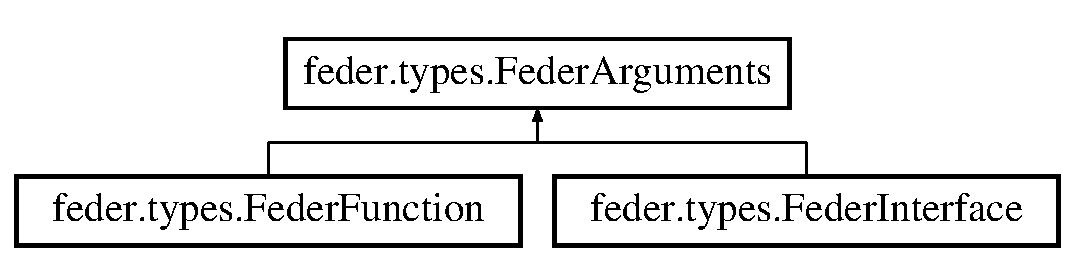
\includegraphics[height=2.000000cm]{interfacefeder_1_1types_1_1FederArguments}
\end{center}
\end{figure}
\subsection*{Public Member Functions}
\begin{DoxyCompactItemize}
\item 
\mbox{\Hypertarget{interfacefeder_1_1types_1_1FederArguments_ab52a621d8a4ac4e5c6c618db36732cc6}\label{interfacefeder_1_1types_1_1FederArguments_ab52a621d8a4ac4e5c6c618db36732cc6}} 
List$<$ \hyperlink{classfeder_1_1types_1_1FederObject}{Feder\+Object} $>$ {\bfseries get\+Arguments} ()
\item 
\mbox{\Hypertarget{interfacefeder_1_1types_1_1FederArguments_a9c26ec99b5be474f308456b536a81b2d}\label{interfacefeder_1_1types_1_1FederArguments_a9c26ec99b5be474f308456b536a81b2d}} 
\hyperlink{classfeder_1_1types_1_1FederBinding}{Feder\+Binding} {\bfseries get\+Return\+Type} ()
\item 
\mbox{\Hypertarget{interfacefeder_1_1types_1_1FederArguments_a528e2baac5fa801623d2d57eadd9f620}\label{interfacefeder_1_1types_1_1FederArguments_a528e2baac5fa801623d2d57eadd9f620}} 
void {\bfseries set\+Return\+Type} (\hyperlink{classfeder_1_1types_1_1FederBinding}{Feder\+Binding} fc)
\item 
\mbox{\Hypertarget{interfacefeder_1_1types_1_1FederArguments_af6c7334cd40b2493ab5c22da624f6024}\label{interfacefeder_1_1types_1_1FederArguments_af6c7334cd40b2493ab5c22da624f6024}} 
String {\bfseries get\+Name} ()
\item 
\mbox{\Hypertarget{interfacefeder_1_1types_1_1FederArguments_a8d9c851eaef82f27a871d57b77311a20}\label{interfacefeder_1_1types_1_1FederArguments_a8d9c851eaef82f27a871d57b77311a20}} 
boolean {\bfseries is\+Equal} (String name, List$<$ \hyperlink{classfeder_1_1types_1_1FederBinding}{Feder\+Binding} $>$ args)
\item 
\mbox{\Hypertarget{interfacefeder_1_1types_1_1FederArguments_aff985816edbc33831f9ecf941f9f5667}\label{interfacefeder_1_1types_1_1FederArguments_aff985816edbc33831f9ecf941f9f5667}} 
String {\bfseries generate\+C\+Name} ()
\item 
\mbox{\Hypertarget{interfacefeder_1_1types_1_1FederArguments_a558b054cc277f7b8795b7651a1c57d7d}\label{interfacefeder_1_1types_1_1FederArguments_a558b054cc277f7b8795b7651a1c57d7d}} 
\hyperlink{classfeder_1_1types_1_1FederBody}{Feder\+Body} {\bfseries get\+Parent} ()
\item 
\mbox{\Hypertarget{interfacefeder_1_1types_1_1FederArguments_ac3501e9f7b11a9ab902f865e6a9dd938}\label{interfacefeder_1_1types_1_1FederArguments_ac3501e9f7b11a9ab902f865e6a9dd938}} 
boolean {\bfseries can\+Be\+Called} ()
\item 
\mbox{\Hypertarget{interfacefeder_1_1types_1_1FederArguments_a04044c9dab7c97b96f840e8c73f459d7}\label{interfacefeder_1_1types_1_1FederArguments_a04044c9dab7c97b96f840e8c73f459d7}} 
boolean {\bfseries is\+Private} ()
\end{DoxyCompactItemize}


\subsection{Detailed Description}
\begin{DoxyAuthor}{Author}
Fionn Langhans 
\end{DoxyAuthor}


The documentation for this interface was generated from the following file\+:\begin{DoxyCompactItemize}
\item 
src/feder/types/Feder\+Arguments.\+java\end{DoxyCompactItemize}

\hypertarget{classfeder_1_1types_1_1FederArray}{}\section{feder.\+types.\+Feder\+Array Class Reference}
\label{classfeder_1_1types_1_1FederArray}\index{feder.\+types.\+Feder\+Array@{feder.\+types.\+Feder\+Array}}
Inheritance diagram for feder.\+types.\+Feder\+Array\+:\begin{figure}[H]
\begin{center}
\leavevmode
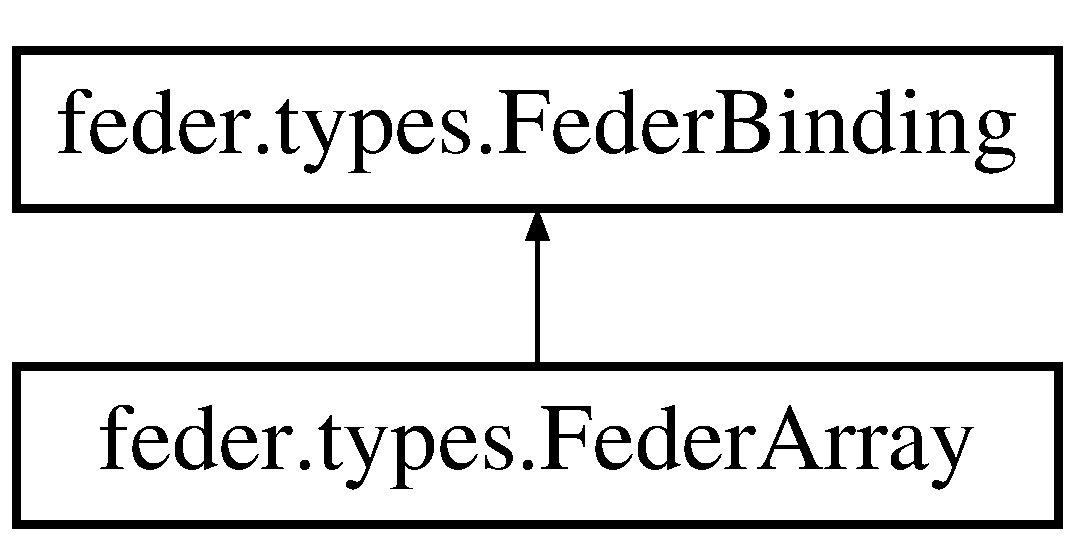
\includegraphics[height=2.000000cm]{classfeder_1_1types_1_1FederArray}
\end{center}
\end{figure}
\subsection*{Public Member Functions}
\begin{DoxyCompactItemize}
\item 
\hyperlink{classfeder_1_1types_1_1FederArray_a0f799437788cc7f8d6beff53667fda6f}{Feder\+Array} (\hyperlink{classfeder_1_1types_1_1FederBinding}{Feder\+Binding} type0)
\item 
boolean \hyperlink{classfeder_1_1types_1_1FederArray_ac6c0b3642d82efecc34be9a73c8447e8}{equals} (Object obj)
\item 
\hyperlink{classfeder_1_1types_1_1FederBinding}{Feder\+Binding} \hyperlink{classfeder_1_1types_1_1FederArray_ae4d5fffefb7cf173ed04a86b4a6c2de0}{get\+Type} ()
\item 
boolean \hyperlink{classfeder_1_1types_1_1FederArray_a62acbf35378415cb9b78823d18d74f59}{is\+Data\+Type} ()
\item 
boolean \hyperlink{classfeder_1_1types_1_1FederArray_a82c7357547d398c09c2437b9bbaedf24}{is\+Interface} ()
\item 
boolean \hyperlink{classfeder_1_1types_1_1FederArray_a2defe214b433edc0169246e2f028c3fc}{is\+Type\+Or\+Interface} ()
\item 
String \hyperlink{classfeder_1_1types_1_1FederArray_a3a03529799560dd4453a2c7091ea6337}{get\+Name} ()
\item 
String \hyperlink{classfeder_1_1types_1_1FederArray_a4928bd58e0ec5c07efdff1ebcef528ff}{get\+Code\+Friendly\+Name} ()
\item 
String \hyperlink{classfeder_1_1types_1_1FederArray_a3a90e3bd9b639374158bc5fd717c824b}{generate\+C\+Name} ()
\item 
boolean \hyperlink{classfeder_1_1types_1_1FederArray_a342cc0011064b863d9524bc90c478ee6}{has\+To\+Build} ()
\item 
void \hyperlink{classfeder_1_1types_1_1FederArray_a44cbed29acf49dde8b64bcc05d3d6943}{set\+Has\+To\+Build} (boolean build)
\item 
\hyperlink{classfeder_1_1types_1_1FederBody}{Feder\+Body} \hyperlink{classfeder_1_1types_1_1FederArray_a1b547ac37dd2072afb7bd7360342f1f1}{get\+Parent} ()
\end{DoxyCompactItemize}
\subsection*{Additional Inherited Members}


\subsection{Detailed Description}
This class should handle arrays created for objects (primitive datatype objects and objects created from classes)

\begin{DoxyAuthor}{Author}
Fionn Langhans 
\end{DoxyAuthor}


\subsection{Constructor \& Destructor Documentation}
\mbox{\Hypertarget{classfeder_1_1types_1_1FederArray_a0f799437788cc7f8d6beff53667fda6f}\label{classfeder_1_1types_1_1FederArray_a0f799437788cc7f8d6beff53667fda6f}} 
\index{feder\+::types\+::\+Feder\+Array@{feder\+::types\+::\+Feder\+Array}!Feder\+Array@{Feder\+Array}}
\index{Feder\+Array@{Feder\+Array}!feder\+::types\+::\+Feder\+Array@{feder\+::types\+::\+Feder\+Array}}
\subsubsection{\texorpdfstring{Feder\+Array()}{FederArray()}}
{\footnotesize\ttfamily feder.\+types.\+Feder\+Array.\+Feder\+Array (\begin{DoxyParamCaption}\item[{\hyperlink{classfeder_1_1types_1_1FederBinding}{Feder\+Binding}}]{type0 }\end{DoxyParamCaption})}


\begin{DoxyParams}{Parameters}
{\em type0} & The type of the array \\
\hline
\end{DoxyParams}


\subsection{Member Function Documentation}
\mbox{\Hypertarget{classfeder_1_1types_1_1FederArray_ac6c0b3642d82efecc34be9a73c8447e8}\label{classfeder_1_1types_1_1FederArray_ac6c0b3642d82efecc34be9a73c8447e8}} 
\index{feder\+::types\+::\+Feder\+Array@{feder\+::types\+::\+Feder\+Array}!equals@{equals}}
\index{equals@{equals}!feder\+::types\+::\+Feder\+Array@{feder\+::types\+::\+Feder\+Array}}
\subsubsection{\texorpdfstring{equals()}{equals()}}
{\footnotesize\ttfamily boolean feder.\+types.\+Feder\+Array.\+equals (\begin{DoxyParamCaption}\item[{Object}]{obj }\end{DoxyParamCaption})}

\begin{DoxyReturn}{Returns}
Returns true if obj is an array and if the array has the same type as this object 
\end{DoxyReturn}
\mbox{\Hypertarget{classfeder_1_1types_1_1FederArray_a3a90e3bd9b639374158bc5fd717c824b}\label{classfeder_1_1types_1_1FederArray_a3a90e3bd9b639374158bc5fd717c824b}} 
\index{feder\+::types\+::\+Feder\+Array@{feder\+::types\+::\+Feder\+Array}!generate\+C\+Name@{generate\+C\+Name}}
\index{generate\+C\+Name@{generate\+C\+Name}!feder\+::types\+::\+Feder\+Array@{feder\+::types\+::\+Feder\+Array}}
\subsubsection{\texorpdfstring{generate\+C\+Name()}{generateCName()}}
{\footnotesize\ttfamily String feder.\+types.\+Feder\+Array.\+generate\+C\+Name (\begin{DoxyParamCaption}{ }\end{DoxyParamCaption})}

\begin{DoxyReturn}{Returns}
Returns the name to use in C (the native language) 
\end{DoxyReturn}
\mbox{\Hypertarget{classfeder_1_1types_1_1FederArray_a4928bd58e0ec5c07efdff1ebcef528ff}\label{classfeder_1_1types_1_1FederArray_a4928bd58e0ec5c07efdff1ebcef528ff}} 
\index{feder\+::types\+::\+Feder\+Array@{feder\+::types\+::\+Feder\+Array}!get\+Code\+Friendly\+Name@{get\+Code\+Friendly\+Name}}
\index{get\+Code\+Friendly\+Name@{get\+Code\+Friendly\+Name}!feder\+::types\+::\+Feder\+Array@{feder\+::types\+::\+Feder\+Array}}
\subsubsection{\texorpdfstring{get\+Code\+Friendly\+Name()}{getCodeFriendlyName()}}
{\footnotesize\ttfamily String feder.\+types.\+Feder\+Array.\+get\+Code\+Friendly\+Name (\begin{DoxyParamCaption}{ }\end{DoxyParamCaption})}

\begin{DoxyReturn}{Returns}
Returns the name of this object (in a code-\/friendly way) 
\end{DoxyReturn}
\mbox{\Hypertarget{classfeder_1_1types_1_1FederArray_a3a03529799560dd4453a2c7091ea6337}\label{classfeder_1_1types_1_1FederArray_a3a03529799560dd4453a2c7091ea6337}} 
\index{feder\+::types\+::\+Feder\+Array@{feder\+::types\+::\+Feder\+Array}!get\+Name@{get\+Name}}
\index{get\+Name@{get\+Name}!feder\+::types\+::\+Feder\+Array@{feder\+::types\+::\+Feder\+Array}}
\subsubsection{\texorpdfstring{get\+Name()}{getName()}}
{\footnotesize\ttfamily String feder.\+types.\+Feder\+Array.\+get\+Name (\begin{DoxyParamCaption}{ }\end{DoxyParamCaption})}

\begin{DoxyReturn}{Returns}
Returns the name of this object 
\end{DoxyReturn}
\mbox{\Hypertarget{classfeder_1_1types_1_1FederArray_a1b547ac37dd2072afb7bd7360342f1f1}\label{classfeder_1_1types_1_1FederArray_a1b547ac37dd2072afb7bd7360342f1f1}} 
\index{feder\+::types\+::\+Feder\+Array@{feder\+::types\+::\+Feder\+Array}!get\+Parent@{get\+Parent}}
\index{get\+Parent@{get\+Parent}!feder\+::types\+::\+Feder\+Array@{feder\+::types\+::\+Feder\+Array}}
\subsubsection{\texorpdfstring{get\+Parent()}{getParent()}}
{\footnotesize\ttfamily \hyperlink{classfeder_1_1types_1_1FederBody}{Feder\+Body} feder.\+types.\+Feder\+Array.\+get\+Parent (\begin{DoxyParamCaption}{ }\end{DoxyParamCaption})}

\begin{DoxyReturn}{Returns}
Returns null 
\end{DoxyReturn}
\mbox{\Hypertarget{classfeder_1_1types_1_1FederArray_ae4d5fffefb7cf173ed04a86b4a6c2de0}\label{classfeder_1_1types_1_1FederArray_ae4d5fffefb7cf173ed04a86b4a6c2de0}} 
\index{feder\+::types\+::\+Feder\+Array@{feder\+::types\+::\+Feder\+Array}!get\+Type@{get\+Type}}
\index{get\+Type@{get\+Type}!feder\+::types\+::\+Feder\+Array@{feder\+::types\+::\+Feder\+Array}}
\subsubsection{\texorpdfstring{get\+Type()}{getType()}}
{\footnotesize\ttfamily \hyperlink{classfeder_1_1types_1_1FederBinding}{Feder\+Binding} feder.\+types.\+Feder\+Array.\+get\+Type (\begin{DoxyParamCaption}{ }\end{DoxyParamCaption})}

\begin{DoxyReturn}{Returns}
Returns the type of the object 
\end{DoxyReturn}
\mbox{\Hypertarget{classfeder_1_1types_1_1FederArray_a342cc0011064b863d9524bc90c478ee6}\label{classfeder_1_1types_1_1FederArray_a342cc0011064b863d9524bc90c478ee6}} 
\index{feder\+::types\+::\+Feder\+Array@{feder\+::types\+::\+Feder\+Array}!has\+To\+Build@{has\+To\+Build}}
\index{has\+To\+Build@{has\+To\+Build}!feder\+::types\+::\+Feder\+Array@{feder\+::types\+::\+Feder\+Array}}
\subsubsection{\texorpdfstring{has\+To\+Build()}{hasToBuild()}}
{\footnotesize\ttfamily boolean feder.\+types.\+Feder\+Array.\+has\+To\+Build (\begin{DoxyParamCaption}{ }\end{DoxyParamCaption})}

\begin{DoxyReturn}{Returns}
Always returns false (mustn\textquotesingle{}t be build) 
\end{DoxyReturn}
\mbox{\Hypertarget{classfeder_1_1types_1_1FederArray_a62acbf35378415cb9b78823d18d74f59}\label{classfeder_1_1types_1_1FederArray_a62acbf35378415cb9b78823d18d74f59}} 
\index{feder\+::types\+::\+Feder\+Array@{feder\+::types\+::\+Feder\+Array}!is\+Data\+Type@{is\+Data\+Type}}
\index{is\+Data\+Type@{is\+Data\+Type}!feder\+::types\+::\+Feder\+Array@{feder\+::types\+::\+Feder\+Array}}
\subsubsection{\texorpdfstring{is\+Data\+Type()}{isDataType()}}
{\footnotesize\ttfamily boolean feder.\+types.\+Feder\+Array.\+is\+Data\+Type (\begin{DoxyParamCaption}{ }\end{DoxyParamCaption})}

\begin{DoxyReturn}{Returns}
Returns true if the array\textquotesingle{}s type is a datatype 
\end{DoxyReturn}
\mbox{\Hypertarget{classfeder_1_1types_1_1FederArray_a82c7357547d398c09c2437b9bbaedf24}\label{classfeder_1_1types_1_1FederArray_a82c7357547d398c09c2437b9bbaedf24}} 
\index{feder\+::types\+::\+Feder\+Array@{feder\+::types\+::\+Feder\+Array}!is\+Interface@{is\+Interface}}
\index{is\+Interface@{is\+Interface}!feder\+::types\+::\+Feder\+Array@{feder\+::types\+::\+Feder\+Array}}
\subsubsection{\texorpdfstring{is\+Interface()}{isInterface()}}
{\footnotesize\ttfamily boolean feder.\+types.\+Feder\+Array.\+is\+Interface (\begin{DoxyParamCaption}{ }\end{DoxyParamCaption})}

\begin{DoxyReturn}{Returns}
Returns true if the array\textquotesingle{}s type is an interface 
\end{DoxyReturn}
\mbox{\Hypertarget{classfeder_1_1types_1_1FederArray_a2defe214b433edc0169246e2f028c3fc}\label{classfeder_1_1types_1_1FederArray_a2defe214b433edc0169246e2f028c3fc}} 
\index{feder\+::types\+::\+Feder\+Array@{feder\+::types\+::\+Feder\+Array}!is\+Type\+Or\+Interface@{is\+Type\+Or\+Interface}}
\index{is\+Type\+Or\+Interface@{is\+Type\+Or\+Interface}!feder\+::types\+::\+Feder\+Array@{feder\+::types\+::\+Feder\+Array}}
\subsubsection{\texorpdfstring{is\+Type\+Or\+Interface()}{isTypeOrInterface()}}
{\footnotesize\ttfamily boolean feder.\+types.\+Feder\+Array.\+is\+Type\+Or\+Interface (\begin{DoxyParamCaption}{ }\end{DoxyParamCaption})}

\begin{DoxyReturn}{Returns}
Returns true, if the array\textquotesingle{}s type is an interface or datatype 
\end{DoxyReturn}
\mbox{\Hypertarget{classfeder_1_1types_1_1FederArray_a44cbed29acf49dde8b64bcc05d3d6943}\label{classfeder_1_1types_1_1FederArray_a44cbed29acf49dde8b64bcc05d3d6943}} 
\index{feder\+::types\+::\+Feder\+Array@{feder\+::types\+::\+Feder\+Array}!set\+Has\+To\+Build@{set\+Has\+To\+Build}}
\index{set\+Has\+To\+Build@{set\+Has\+To\+Build}!feder\+::types\+::\+Feder\+Array@{feder\+::types\+::\+Feder\+Array}}
\subsubsection{\texorpdfstring{set\+Has\+To\+Build()}{setHasToBuild()}}
{\footnotesize\ttfamily void feder.\+types.\+Feder\+Array.\+set\+Has\+To\+Build (\begin{DoxyParamCaption}\item[{boolean}]{build }\end{DoxyParamCaption})}

This function does nothing 
\begin{DoxyParams}{Parameters}
{\em build} & \\
\hline
\end{DoxyParams}


The documentation for this class was generated from the following file\+:\begin{DoxyCompactItemize}
\item 
src/feder/types/Feder\+Array.\+java\end{DoxyCompactItemize}

\hypertarget{classfeder_1_1types_1_1FederAutomat}{}\section{feder.\+types.\+Feder\+Automat Class Reference}
\label{classfeder_1_1types_1_1FederAutomat}\index{feder.\+types.\+Feder\+Automat@{feder.\+types.\+Feder\+Automat}}
Inheritance diagram for feder.\+types.\+Feder\+Automat\+:\begin{figure}[H]
\begin{center}
\leavevmode
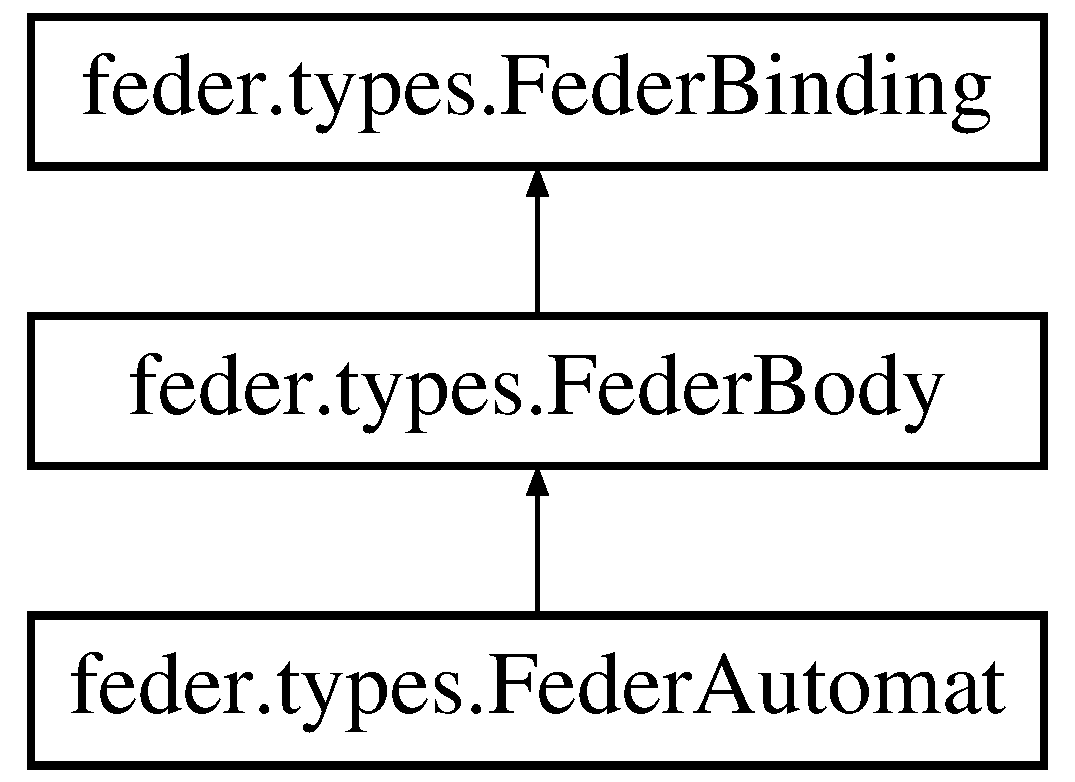
\includegraphics[height=3.000000cm]{classfeder_1_1types_1_1FederAutomat}
\end{center}
\end{figure}
\subsection*{Public Member Functions}
\begin{DoxyCompactItemize}
\item 
\mbox{\Hypertarget{classfeder_1_1types_1_1FederAutomat_ae6a34e03f15ff7621320cd013afd27fa}\label{classfeder_1_1types_1_1FederAutomat_ae6a34e03f15ff7621320cd013afd27fa}} 
{\bfseries Feder\+Automat} (\hyperlink{classfeder_1_1FederCompiler}{Feder\+Compiler} compiler0, \hyperlink{classfeder_1_1types_1_1FederBody}{Feder\+Body} parent0, String type0)
\item 
\mbox{\Hypertarget{classfeder_1_1types_1_1FederAutomat_ab413cf26cfaaa6e2911786ace424aa29}\label{classfeder_1_1types_1_1FederAutomat_ab413cf26cfaaa6e2911786ace424aa29}} 
String {\bfseries get\+Type} ()
\item 
\mbox{\Hypertarget{classfeder_1_1types_1_1FederAutomat_a38830b199a268b46fd7c11fe065e7fbf}\label{classfeder_1_1types_1_1FederAutomat_a38830b199a268b46fd7c11fe065e7fbf}} 
String {\bfseries generate\+C\+Name} ()
\end{DoxyCompactItemize}
\subsection*{Additional Inherited Members}


\subsection{Detailed Description}
Diese Klasse ist für die Syntaxkörper\+: while, if, else, else if

\begin{DoxyAuthor}{Author}
Fionn Langhans 
\end{DoxyAuthor}


The documentation for this class was generated from the following file\+:\begin{DoxyCompactItemize}
\item 
src/feder/types/Feder\+Automat.\+java\end{DoxyCompactItemize}

\hypertarget{classfeder_1_1types_1_1FederBinding}{}\section{feder.\+types.\+Feder\+Binding Class Reference}
\label{classfeder_1_1types_1_1FederBinding}\index{feder.\+types.\+Feder\+Binding@{feder.\+types.\+Feder\+Binding}}
Inheritance diagram for feder.\+types.\+Feder\+Binding\+:\begin{figure}[H]
\begin{center}
\leavevmode
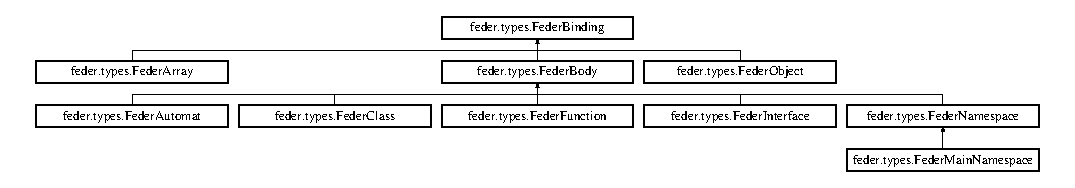
\includegraphics[height=2.074074cm]{classfeder_1_1types_1_1FederBinding}
\end{center}
\end{figure}
\subsection*{Public Member Functions}
\begin{DoxyCompactItemize}
\item 
abstract String \hyperlink{classfeder_1_1types_1_1FederBinding_ab233b4eb1c5fef826e01cfe610447cea}{get\+Name} ()
\item 
abstract String \hyperlink{classfeder_1_1types_1_1FederBinding_a237e4d83da1cee7e4bcaecea513c4b9d}{get\+Code\+Friendly\+Name} ()
\item 
abstract String \hyperlink{classfeder_1_1types_1_1FederBinding_a8a3a3d920f5312db5beff5c82071cb12}{generate\+C\+Name} ()
\item 
abstract boolean \hyperlink{classfeder_1_1types_1_1FederBinding_a72cdcf7fcc293cfadb311c52abffdd00}{has\+To\+Build} ()
\item 
abstract void \hyperlink{classfeder_1_1types_1_1FederBinding_a8c895588a1ab8067b5697ff5c9608fa5}{set\+Has\+To\+Build} (boolean build)
\item 
boolean \hyperlink{classfeder_1_1types_1_1FederBinding_ad5937fb65ae2d25cc075dcf639dcfe04}{is\+Private} ()
\item 
boolean \hyperlink{classfeder_1_1types_1_1FederBinding_a84df88cf32e2d678fc73f8e868477487}{is\+Immutable} ()
\item 
abstract \hyperlink{classfeder_1_1types_1_1FederBody}{Feder\+Body} \hyperlink{classfeder_1_1types_1_1FederBinding_a28620ccaf5f32f1376e6c6bd1d13452d}{get\+Parent} ()
\end{DoxyCompactItemize}
\subsection*{Static Public Member Functions}
\begin{DoxyCompactItemize}
\item 
static boolean \hyperlink{classfeder_1_1types_1_1FederBinding_a25f8e1f9d64b08dc98c7be9bf931e479}{Is\+Garbagable} (\hyperlink{classfeder_1_1types_1_1FederBinding}{Feder\+Binding} bind)
\item 
static boolean \hyperlink{classfeder_1_1types_1_1FederBinding_aefeac9d1325508287fb394ab0a6c54a3}{are\+Same\+Types} (\hyperlink{classfeder_1_1types_1_1FederBinding}{Feder\+Binding} bind0, \hyperlink{classfeder_1_1types_1_1FederBinding}{Feder\+Binding} bind1)
\item 
static boolean \hyperlink{classfeder_1_1types_1_1FederBinding_a2c04e0db9889dacd7ad0c5a839797c2f}{is\+Data\+Type} (\hyperlink{classfeder_1_1types_1_1FederBinding}{Feder\+Binding} binding)
\end{DoxyCompactItemize}


\subsection{Detailed Description}
\begin{DoxyAuthor}{Author}
Fionn Langhans 
\end{DoxyAuthor}


\subsection{Member Function Documentation}
\mbox{\Hypertarget{classfeder_1_1types_1_1FederBinding_aefeac9d1325508287fb394ab0a6c54a3}\label{classfeder_1_1types_1_1FederBinding_aefeac9d1325508287fb394ab0a6c54a3}} 
\index{feder\+::types\+::\+Feder\+Binding@{feder\+::types\+::\+Feder\+Binding}!are\+Same\+Types@{are\+Same\+Types}}
\index{are\+Same\+Types@{are\+Same\+Types}!feder\+::types\+::\+Feder\+Binding@{feder\+::types\+::\+Feder\+Binding}}
\subsubsection{\texorpdfstring{are\+Same\+Types()}{areSameTypes()}}
{\footnotesize\ttfamily static boolean feder.\+types.\+Feder\+Binding.\+are\+Same\+Types (\begin{DoxyParamCaption}\item[{\hyperlink{classfeder_1_1types_1_1FederBinding}{Feder\+Binding}}]{bind0,  }\item[{\hyperlink{classfeder_1_1types_1_1FederBinding}{Feder\+Binding}}]{bind1 }\end{DoxyParamCaption})\hspace{0.3cm}{\ttfamily [static]}}


\begin{DoxyParams}{Parameters}
{\em bind0} & \\
\hline
{\em bind1} & \\
\hline
\end{DoxyParams}
\begin{DoxyReturn}{Returns}
Returns true, if bind0 and bind1 have the same types or are the same (if bind0 or bind1 is null, the result is false). 
\end{DoxyReturn}
\mbox{\Hypertarget{classfeder_1_1types_1_1FederBinding_a8a3a3d920f5312db5beff5c82071cb12}\label{classfeder_1_1types_1_1FederBinding_a8a3a3d920f5312db5beff5c82071cb12}} 
\index{feder\+::types\+::\+Feder\+Binding@{feder\+::types\+::\+Feder\+Binding}!generate\+C\+Name@{generate\+C\+Name}}
\index{generate\+C\+Name@{generate\+C\+Name}!feder\+::types\+::\+Feder\+Binding@{feder\+::types\+::\+Feder\+Binding}}
\subsubsection{\texorpdfstring{generate\+C\+Name()}{generateCName()}}
{\footnotesize\ttfamily abstract String feder.\+types.\+Feder\+Binding.\+generate\+C\+Name (\begin{DoxyParamCaption}{ }\end{DoxyParamCaption})\hspace{0.3cm}{\ttfamily [abstract]}}

\begin{DoxyReturn}{Returns}
Returns the name, which should be used in C. 
\end{DoxyReturn}
\mbox{\Hypertarget{classfeder_1_1types_1_1FederBinding_a237e4d83da1cee7e4bcaecea513c4b9d}\label{classfeder_1_1types_1_1FederBinding_a237e4d83da1cee7e4bcaecea513c4b9d}} 
\index{feder\+::types\+::\+Feder\+Binding@{feder\+::types\+::\+Feder\+Binding}!get\+Code\+Friendly\+Name@{get\+Code\+Friendly\+Name}}
\index{get\+Code\+Friendly\+Name@{get\+Code\+Friendly\+Name}!feder\+::types\+::\+Feder\+Binding@{feder\+::types\+::\+Feder\+Binding}}
\subsubsection{\texorpdfstring{get\+Code\+Friendly\+Name()}{getCodeFriendlyName()}}
{\footnotesize\ttfamily abstract String feder.\+types.\+Feder\+Binding.\+get\+Code\+Friendly\+Name (\begin{DoxyParamCaption}{ }\end{DoxyParamCaption})\hspace{0.3cm}{\ttfamily [abstract]}}

\begin{DoxyReturn}{Returns}
Should return a \textquotesingle{}code friendly\textquotesingle{} name (something like generate\+C\+Name, but compatible to construct bigger names) 
\end{DoxyReturn}
\mbox{\Hypertarget{classfeder_1_1types_1_1FederBinding_ab233b4eb1c5fef826e01cfe610447cea}\label{classfeder_1_1types_1_1FederBinding_ab233b4eb1c5fef826e01cfe610447cea}} 
\index{feder\+::types\+::\+Feder\+Binding@{feder\+::types\+::\+Feder\+Binding}!get\+Name@{get\+Name}}
\index{get\+Name@{get\+Name}!feder\+::types\+::\+Feder\+Binding@{feder\+::types\+::\+Feder\+Binding}}
\subsubsection{\texorpdfstring{get\+Name()}{getName()}}
{\footnotesize\ttfamily abstract String feder.\+types.\+Feder\+Binding.\+get\+Name (\begin{DoxyParamCaption}{ }\end{DoxyParamCaption})\hspace{0.3cm}{\ttfamily [abstract]}}

\begin{DoxyReturn}{Returns}
Should return the name of the binding 
\end{DoxyReturn}
\mbox{\Hypertarget{classfeder_1_1types_1_1FederBinding_a28620ccaf5f32f1376e6c6bd1d13452d}\label{classfeder_1_1types_1_1FederBinding_a28620ccaf5f32f1376e6c6bd1d13452d}} 
\index{feder\+::types\+::\+Feder\+Binding@{feder\+::types\+::\+Feder\+Binding}!get\+Parent@{get\+Parent}}
\index{get\+Parent@{get\+Parent}!feder\+::types\+::\+Feder\+Binding@{feder\+::types\+::\+Feder\+Binding}}
\subsubsection{\texorpdfstring{get\+Parent()}{getParent()}}
{\footnotesize\ttfamily abstract \hyperlink{classfeder_1_1types_1_1FederBody}{Feder\+Body} feder.\+types.\+Feder\+Binding.\+get\+Parent (\begin{DoxyParamCaption}{ }\end{DoxyParamCaption})\hspace{0.3cm}{\ttfamily [abstract]}}

\begin{DoxyReturn}{Returns}
Should return the parent of the binding 
\end{DoxyReturn}
\mbox{\Hypertarget{classfeder_1_1types_1_1FederBinding_a72cdcf7fcc293cfadb311c52abffdd00}\label{classfeder_1_1types_1_1FederBinding_a72cdcf7fcc293cfadb311c52abffdd00}} 
\index{feder\+::types\+::\+Feder\+Binding@{feder\+::types\+::\+Feder\+Binding}!has\+To\+Build@{has\+To\+Build}}
\index{has\+To\+Build@{has\+To\+Build}!feder\+::types\+::\+Feder\+Binding@{feder\+::types\+::\+Feder\+Binding}}
\subsubsection{\texorpdfstring{has\+To\+Build()}{hasToBuild()}}
{\footnotesize\ttfamily abstract boolean feder.\+types.\+Feder\+Binding.\+has\+To\+Build (\begin{DoxyParamCaption}{ }\end{DoxyParamCaption})\hspace{0.3cm}{\ttfamily [abstract]}}

\begin{DoxyReturn}{Returns}
Should return true, if the binding has to be build. 
\end{DoxyReturn}
\mbox{\Hypertarget{classfeder_1_1types_1_1FederBinding_a2c04e0db9889dacd7ad0c5a839797c2f}\label{classfeder_1_1types_1_1FederBinding_a2c04e0db9889dacd7ad0c5a839797c2f}} 
\index{feder\+::types\+::\+Feder\+Binding@{feder\+::types\+::\+Feder\+Binding}!is\+Data\+Type@{is\+Data\+Type}}
\index{is\+Data\+Type@{is\+Data\+Type}!feder\+::types\+::\+Feder\+Binding@{feder\+::types\+::\+Feder\+Binding}}
\subsubsection{\texorpdfstring{is\+Data\+Type()}{isDataType()}}
{\footnotesize\ttfamily static boolean feder.\+types.\+Feder\+Binding.\+is\+Data\+Type (\begin{DoxyParamCaption}\item[{\hyperlink{classfeder_1_1types_1_1FederBinding}{Feder\+Binding}}]{binding }\end{DoxyParamCaption})\hspace{0.3cm}{\ttfamily [static]}}


\begin{DoxyParams}{Parameters}
{\em binding} & \\
\hline
\end{DoxyParams}
\begin{DoxyReturn}{Returns}
Returns true, if binding is a datatype. 
\end{DoxyReturn}
\mbox{\Hypertarget{classfeder_1_1types_1_1FederBinding_a25f8e1f9d64b08dc98c7be9bf931e479}\label{classfeder_1_1types_1_1FederBinding_a25f8e1f9d64b08dc98c7be9bf931e479}} 
\index{feder\+::types\+::\+Feder\+Binding@{feder\+::types\+::\+Feder\+Binding}!Is\+Garbagable@{Is\+Garbagable}}
\index{Is\+Garbagable@{Is\+Garbagable}!feder\+::types\+::\+Feder\+Binding@{feder\+::types\+::\+Feder\+Binding}}
\subsubsection{\texorpdfstring{Is\+Garbagable()}{IsGarbagable()}}
{\footnotesize\ttfamily static boolean feder.\+types.\+Feder\+Binding.\+Is\+Garbagable (\begin{DoxyParamCaption}\item[{\hyperlink{classfeder_1_1types_1_1FederBinding}{Feder\+Binding}}]{bind }\end{DoxyParamCaption})\hspace{0.3cm}{\ttfamily [static]}}


\begin{DoxyParams}{Parameters}
{\em bind} & \\
\hline
\end{DoxyParams}
\begin{DoxyReturn}{Returns}
Returns true, if the binding \textquotesingle{}bind\textquotesingle{} is garbageable (true if class and not datatype or if type is array) 
\end{DoxyReturn}
\mbox{\Hypertarget{classfeder_1_1types_1_1FederBinding_a84df88cf32e2d678fc73f8e868477487}\label{classfeder_1_1types_1_1FederBinding_a84df88cf32e2d678fc73f8e868477487}} 
\index{feder\+::types\+::\+Feder\+Binding@{feder\+::types\+::\+Feder\+Binding}!is\+Immutable@{is\+Immutable}}
\index{is\+Immutable@{is\+Immutable}!feder\+::types\+::\+Feder\+Binding@{feder\+::types\+::\+Feder\+Binding}}
\subsubsection{\texorpdfstring{is\+Immutable()}{isImmutable()}}
{\footnotesize\ttfamily boolean feder.\+types.\+Feder\+Binding.\+is\+Immutable (\begin{DoxyParamCaption}{ }\end{DoxyParamCaption})}

\begin{DoxyReturn}{Returns}
Returns true, if the binding should be immutable 
\end{DoxyReturn}
\mbox{\Hypertarget{classfeder_1_1types_1_1FederBinding_ad5937fb65ae2d25cc075dcf639dcfe04}\label{classfeder_1_1types_1_1FederBinding_ad5937fb65ae2d25cc075dcf639dcfe04}} 
\index{feder\+::types\+::\+Feder\+Binding@{feder\+::types\+::\+Feder\+Binding}!is\+Private@{is\+Private}}
\index{is\+Private@{is\+Private}!feder\+::types\+::\+Feder\+Binding@{feder\+::types\+::\+Feder\+Binding}}
\subsubsection{\texorpdfstring{is\+Private()}{isPrivate()}}
{\footnotesize\ttfamily boolean feder.\+types.\+Feder\+Binding.\+is\+Private (\begin{DoxyParamCaption}{ }\end{DoxyParamCaption})}

\begin{DoxyReturn}{Returns}
Returns true, if the binding should be private 
\end{DoxyReturn}
\mbox{\Hypertarget{classfeder_1_1types_1_1FederBinding_a8c895588a1ab8067b5697ff5c9608fa5}\label{classfeder_1_1types_1_1FederBinding_a8c895588a1ab8067b5697ff5c9608fa5}} 
\index{feder\+::types\+::\+Feder\+Binding@{feder\+::types\+::\+Feder\+Binding}!set\+Has\+To\+Build@{set\+Has\+To\+Build}}
\index{set\+Has\+To\+Build@{set\+Has\+To\+Build}!feder\+::types\+::\+Feder\+Binding@{feder\+::types\+::\+Feder\+Binding}}
\subsubsection{\texorpdfstring{set\+Has\+To\+Build()}{setHasToBuild()}}
{\footnotesize\ttfamily abstract void feder.\+types.\+Feder\+Binding.\+set\+Has\+To\+Build (\begin{DoxyParamCaption}\item[{boolean}]{build }\end{DoxyParamCaption})\hspace{0.3cm}{\ttfamily [abstract]}}


\begin{DoxyParams}{Parameters}
{\em build} & You probably want to set this to \textquotesingle{}false\textquotesingle{} \\
\hline
\end{DoxyParams}


The documentation for this class was generated from the following file\+:\begin{DoxyCompactItemize}
\item 
src/feder/types/Feder\+Binding.\+java\end{DoxyCompactItemize}

\hypertarget{classfeder_1_1types_1_1FederBody}{}\section{feder.\+types.\+Feder\+Body Class Reference}
\label{classfeder_1_1types_1_1FederBody}\index{feder.\+types.\+Feder\+Body@{feder.\+types.\+Feder\+Body}}
Inheritance diagram for feder.\+types.\+Feder\+Body\+:\begin{figure}[H]
\begin{center}
\leavevmode
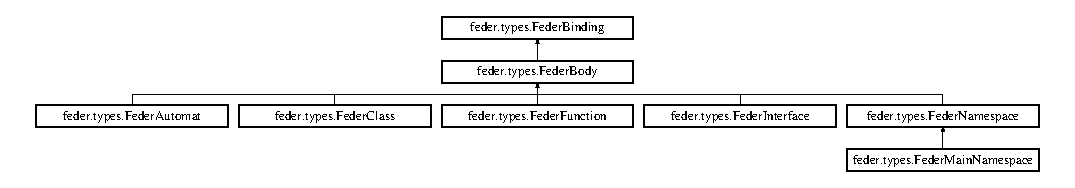
\includegraphics[height=2.074074cm]{classfeder_1_1types_1_1FederBody}
\end{center}
\end{figure}
\subsection*{Public Member Functions}
\begin{DoxyCompactItemize}
\item 
boolean \hyperlink{classfeder_1_1types_1_1FederBody_a8b34fc8b43bba9c859b9e7dc437c3983}{has\+To\+Build} ()
\item 
void \hyperlink{classfeder_1_1types_1_1FederBody_a7368596d9fcc12b30d3c21e69cfee5d6}{set\+Has\+To\+Build} (boolean b)
\item 
void \hyperlink{classfeder_1_1types_1_1FederBody_a38b513fed4f62a653f7dd5a8a8dcca96}{new\+Assume} (\hyperlink{classfeder_1_1types_1_1FederBinding}{Feder\+Binding} key, \hyperlink{classfeder_1_1types_1_1FederBinding}{Feder\+Binding} value)
\item 
void \hyperlink{classfeder_1_1types_1_1FederBody_a2f7b7c8ee314c534f56731e7ee7dbacc}{reset\+Assume} ()
\item 
\hyperlink{classfeder_1_1types_1_1FederBody_a2c3c09316750c434564ad48b7915fe62}{Feder\+Body} (\hyperlink{classfeder_1_1FederCompiler}{Feder\+Compiler} compiler0, String name0, \hyperlink{classfeder_1_1types_1_1FederBody}{Feder\+Body} parent0, Class$<$? extends \hyperlink{classfeder_1_1types_1_1FederBinding}{Feder\+Binding} $>$... blacklist\+\_\+classes0)
\item 
\hyperlink{classfeder_1_1FederCompiler}{Feder\+Compiler} \hyperlink{classfeder_1_1types_1_1FederBody_a1b33bcff46a927796e956f6ded84764d}{get\+Compiler} ()
\item 
List$<$ \hyperlink{classfeder_1_1types_1_1FederBinding}{Feder\+Binding} $>$ \hyperlink{classfeder_1_1types_1_1FederBody_a8e867ab209301d58c984c4e27d324325}{get\+Bindings} ()
\item 
void \hyperlink{classfeder_1_1types_1_1FederBody_a85edfceb1e2b9828d5d6b854a167f221}{add\+Binding} (\hyperlink{classfeder_1_1types_1_1FederBinding}{Feder\+Binding} binding)
\item 
void \hyperlink{classfeder_1_1types_1_1FederBody_a7651c132103a25c4450ccdc3de8df2a3}{insert\+Binding} (\hyperlink{classfeder_1_1types_1_1FederBinding}{Feder\+Binding} binding, int pos)
\item 
String \hyperlink{classfeder_1_1types_1_1FederBody_a8d37894b7118c7cd28dc840703b69fed}{get\+Code\+Friendly\+Name} ()
\item 
\hyperlink{classfeder_1_1types_1_1FederBinding}{Feder\+Binding} \hyperlink{classfeder_1_1types_1_1FederBody_a3102ab9961f4c629236351161c5f4ccc}{get\+Binding} (\hyperlink{classfeder_1_1types_1_1FederBody}{Feder\+Body} requestingbody, String name0, boolean allow\+Parent)
\item 
\hyperlink{classfeder_1_1types_1_1FederBody}{Feder\+Body} \hyperlink{classfeder_1_1types_1_1FederBody_abd9f05e0abc4dd97e9ef3e6df440968b}{get\+Parent} ()
\item 
void \hyperlink{classfeder_1_1types_1_1FederBody_a0c773c1b19c9fb19e27270674ebd54e0}{set\+Parent} (\hyperlink{classfeder_1_1types_1_1FederBody}{Feder\+Body} parent0)
\item 
String \hyperlink{classfeder_1_1types_1_1FederBody_a7d32aee068f32d2cc132df84b32f16c2}{get\+Name} ()
\item 
List$<$ \hyperlink{classfeder_1_1types_1_1FederNamespace}{Feder\+Namespace} $>$ \hyperlink{classfeder_1_1types_1_1FederBody_a8921df8000dc7b7c5894f4871f162cfb}{get\+Namespaces} ()
\item 
String \hyperlink{classfeder_1_1types_1_1FederBody_aa71817818b5b4c8ae05e3e520240cbb3}{get\+Namespaces\+To\+String} ()
\item 
String \hyperlink{classfeder_1_1types_1_1FederBody_a0ced009ee53ed04b803fed0b2237538c}{get\+Namespaces\+To\+Normal\+String} ()
\item 
String \hyperlink{classfeder_1_1types_1_1FederBody_ab31ab3308f48585665e6367f776c1d71}{to\+Written\+String} ()
\item 
List$<$ \hyperlink{classfeder_1_1types_1_1FederBinding}{Feder\+Binding} $>$ \hyperlink{classfeder_1_1types_1_1FederBody_a119382c9410b28689420735a3863d08f}{get\+Binding\+From\+List} (\hyperlink{classfeder_1_1types_1_1FederBody}{Feder\+Body} requestingbody, List$<$ String $>$ list)
\item 
\hyperlink{interfacefeder_1_1types_1_1FederArguments}{Feder\+Arguments} \hyperlink{classfeder_1_1types_1_1FederBody_a206376c3ed2efe89fe570f996118ce29}{get\+Function} (\hyperlink{classfeder_1_1types_1_1FederBody}{Feder\+Body} requestingbody, String name1, List$<$ \hyperlink{classfeder_1_1types_1_1FederBinding}{Feder\+Binding} $>$ arguments, boolean allow\+Parent)
\item 
\hyperlink{classfeder_1_1types_1_1FederClass}{Feder\+Class} \hyperlink{classfeder_1_1types_1_1FederBody_a31c99a87dddae5d4e5b5d1a7bc0af98f}{get\+Class\+In\+Body} ()
\item 
int \hyperlink{classfeder_1_1types_1_1FederBody_a578373bc7ed4a41102f7bf8ef1aa1c88}{get\+Parents\+Count} ()
\item 
String \hyperlink{classfeder_1_1types_1_1FederBody_a3a0f5cccf7ec89b1e0af8f958236c9aa}{in\+Front\+Of\+Syntax} ()
\item 
\hyperlink{classfeder_1_1types_1_1FederFunction}{Feder\+Function} \hyperlink{classfeder_1_1types_1_1FederBody_a95db3cb467da96aec741f286042e7bbc}{get\+Upper\+Function} ()
\item 
\hyperlink{classfeder_1_1types_1_1FederNamespace}{Feder\+Namespace} \hyperlink{classfeder_1_1types_1_1FederBody_a8ab3e023c05b44cdfbd4e7f22aa9844b}{get\+Upper\+Namespace} ()
\item 
boolean \hyperlink{classfeder_1_1types_1_1FederBody_adf3772434a48f9ac4d203a5e8b7c11fc}{is\+In\+Loop} ()
\item 
boolean \hyperlink{classfeder_1_1types_1_1FederBody_ab3f37b7b8ea9806ea13856f993e11902}{is\+In\+Function} ()
\item 
boolean \hyperlink{classfeder_1_1types_1_1FederBody_a0947a2d7c8ada0a1960fc1536c25731b}{is\+In\+Namespace} ()
\item 
\hyperlink{classfeder_1_1types_1_1FederBody}{Feder\+Body} \hyperlink{classfeder_1_1types_1_1FederBody_ac69fba3b468b2f0ab66d7a87cc501da6}{get\+Main\+Body} ()
\item 
\hyperlink{classfeder_1_1types_1_1FederMainNamespace}{Feder\+Main\+Namespace} \hyperlink{classfeder_1_1types_1_1FederBody_a88b8e80235ad8b5b8dc92e7e2e9daaca}{get\+Main\+Namespace} ()
\end{DoxyCompactItemize}
\subsection*{Static Public Member Functions}
\begin{DoxyCompactItemize}
\item 
static \hyperlink{classfeder_1_1types_1_1FederClass}{Feder\+Class} \hyperlink{classfeder_1_1types_1_1FederBody_a7e2624283680ec9dfd0a6816da173540}{get\+Class\+In\+Binding} (\hyperlink{classfeder_1_1types_1_1FederBinding}{Feder\+Binding} binding)
\end{DoxyCompactItemize}
\subsection*{Public Attributes}
\begin{DoxyCompactItemize}
\item 
String\+Builder \hyperlink{classfeder_1_1types_1_1FederBody_a4735b22113042ca2cb86572c6b982e25}{compile\+\_\+file\+\_\+text} = new String\+Builder()
\item 
String\+Builder \hyperlink{classfeder_1_1types_1_1FederBody_ac834fd62ff90240400dfcddc5e1f4c1f}{header\+\_\+file\+\_\+text\+\_\+beg} = new String\+Builder()
\item 
String\+Builder \hyperlink{classfeder_1_1types_1_1FederBody_af6ffc7aab354eec7f4ea73decc489f24}{header\+\_\+file\+\_\+text} = new String\+Builder()
\item 
String\+Builder \hyperlink{classfeder_1_1types_1_1FederBody_a765165e7c3baabd64219b1968ff6beab}{header\+\_\+file\+\_\+text\+\_\+end} = new String\+Builder()
\item 
boolean \hyperlink{classfeder_1_1types_1_1FederBody_a4602832966e1e3fa19cf19f06a69aa07}{return\+Came} = false
\item 
List$<$ \hyperlink{classfeder_1_1types_1_1FederBody}{Feder\+Body} $>$ \hyperlink{classfeder_1_1types_1_1FederBody_a833aa456985af005fa923bc8771cca7a}{depend\+Bodies} = new Linked\+List$<$$>$()
\end{DoxyCompactItemize}
\subsection*{Protected Member Functions}
\begin{DoxyCompactItemize}
\item 
\hyperlink{classfeder_1_1types_1_1FederBinding}{Feder\+Binding} \hyperlink{classfeder_1_1types_1_1FederBody_a0e81024eaf979b1dc4b0b279885380c8}{get\+Binding} (\hyperlink{classfeder_1_1types_1_1FederBody}{Feder\+Body} requestingbody, String name0, boolean allow\+Parent, List$<$ \hyperlink{classfeder_1_1types_1_1FederBody}{Feder\+Body} $>$ bodies\+Checked)
\item 
\hyperlink{interfacefeder_1_1types_1_1FederArguments}{Feder\+Arguments} \hyperlink{classfeder_1_1types_1_1FederBody_ae2d7a27c12b0dbd096ec638792d69adc}{get\+Function} (\hyperlink{classfeder_1_1types_1_1FederBody}{Feder\+Body} requestingbody, String name1, List$<$ \hyperlink{classfeder_1_1types_1_1FederBinding}{Feder\+Binding} $>$ arguments, boolean allow\+Parent, List$<$ \hyperlink{classfeder_1_1types_1_1FederBody}{Feder\+Body} $>$ bodies\+Checked)
\end{DoxyCompactItemize}
\subsection*{Protected Attributes}
\begin{DoxyCompactItemize}
\item 
Class$<$? extends \hyperlink{classfeder_1_1types_1_1FederBinding}{Feder\+Binding} $>$ \mbox{[}$\,$\mbox{]} \hyperlink{classfeder_1_1types_1_1FederBody_a0408b11249a7eaa41bd71fdfba5bbfb9}{blacklist\+\_\+classes}
\end{DoxyCompactItemize}


\subsection{Detailed Description}
\begin{DoxyAuthor}{Author}
Fionn Langhans 
\end{DoxyAuthor}


\subsection{Constructor \& Destructor Documentation}
\mbox{\Hypertarget{classfeder_1_1types_1_1FederBody_a2c3c09316750c434564ad48b7915fe62}\label{classfeder_1_1types_1_1FederBody_a2c3c09316750c434564ad48b7915fe62}} 
\index{feder\+::types\+::\+Feder\+Body@{feder\+::types\+::\+Feder\+Body}!Feder\+Body@{Feder\+Body}}
\index{Feder\+Body@{Feder\+Body}!feder\+::types\+::\+Feder\+Body@{feder\+::types\+::\+Feder\+Body}}
\subsubsection{\texorpdfstring{Feder\+Body()}{FederBody()}}
{\footnotesize\ttfamily feder.\+types.\+Feder\+Body.\+Feder\+Body (\begin{DoxyParamCaption}\item[{\hyperlink{classfeder_1_1FederCompiler}{Feder\+Compiler}}]{compiler0,  }\item[{String}]{name0,  }\item[{\hyperlink{classfeder_1_1types_1_1FederBody}{Feder\+Body}}]{parent0,  }\item[{Class$<$? extends \hyperlink{classfeder_1_1types_1_1FederBinding}{Feder\+Binding} $>$...}]{blacklist\+\_\+classes0 }\end{DoxyParamCaption})}


\begin{DoxyParams}{Parameters}
{\em compiler0} & compiler instance to use \\
\hline
{\em name0} & The name of the body (T\+HE binding) \\
\hline
{\em parent0} & parent of the body \\
\hline
{\em blacklist\+\_\+classes0} & blacklisted classes \\
\hline
\end{DoxyParams}


\subsection{Member Function Documentation}
\mbox{\Hypertarget{classfeder_1_1types_1_1FederBody_a85edfceb1e2b9828d5d6b854a167f221}\label{classfeder_1_1types_1_1FederBody_a85edfceb1e2b9828d5d6b854a167f221}} 
\index{feder\+::types\+::\+Feder\+Body@{feder\+::types\+::\+Feder\+Body}!add\+Binding@{add\+Binding}}
\index{add\+Binding@{add\+Binding}!feder\+::types\+::\+Feder\+Body@{feder\+::types\+::\+Feder\+Body}}
\subsubsection{\texorpdfstring{add\+Binding()}{addBinding()}}
{\footnotesize\ttfamily void feder.\+types.\+Feder\+Body.\+add\+Binding (\begin{DoxyParamCaption}\item[{\hyperlink{classfeder_1_1types_1_1FederBinding}{Feder\+Binding}}]{binding }\end{DoxyParamCaption})}

Add a child to the body 
\begin{DoxyParams}{Parameters}
{\em binding} & The child (optionally has this as parent) \\
\hline
\end{DoxyParams}
\mbox{\Hypertarget{classfeder_1_1types_1_1FederBody_a3102ab9961f4c629236351161c5f4ccc}\label{classfeder_1_1types_1_1FederBody_a3102ab9961f4c629236351161c5f4ccc}} 
\index{feder\+::types\+::\+Feder\+Body@{feder\+::types\+::\+Feder\+Body}!get\+Binding@{get\+Binding}}
\index{get\+Binding@{get\+Binding}!feder\+::types\+::\+Feder\+Body@{feder\+::types\+::\+Feder\+Body}}
\subsubsection{\texorpdfstring{get\+Binding()}{getBinding()}\hspace{0.1cm}{\footnotesize\ttfamily [1/2]}}
{\footnotesize\ttfamily \hyperlink{classfeder_1_1types_1_1FederBinding}{Feder\+Binding} feder.\+types.\+Feder\+Body.\+get\+Binding (\begin{DoxyParamCaption}\item[{\hyperlink{classfeder_1_1types_1_1FederBody}{Feder\+Body}}]{requestingbody,  }\item[{String}]{name0,  }\item[{boolean}]{allow\+Parent }\end{DoxyParamCaption})}


\begin{DoxyParams}{Parameters}
{\em requestingbody} & The body which is requesting. \\
\hline
{\em name0} & The name to search. \\
\hline
{\em allow\+Parent} & Allow the method to search in parents. \\
\hline
\end{DoxyParams}
\begin{DoxyReturn}{Returns}
Returns a fitting binding. If nothing was found \textquotesingle{}null\textquotesingle{}. 
\end{DoxyReturn}
\mbox{\Hypertarget{classfeder_1_1types_1_1FederBody_a0e81024eaf979b1dc4b0b279885380c8}\label{classfeder_1_1types_1_1FederBody_a0e81024eaf979b1dc4b0b279885380c8}} 
\index{feder\+::types\+::\+Feder\+Body@{feder\+::types\+::\+Feder\+Body}!get\+Binding@{get\+Binding}}
\index{get\+Binding@{get\+Binding}!feder\+::types\+::\+Feder\+Body@{feder\+::types\+::\+Feder\+Body}}
\subsubsection{\texorpdfstring{get\+Binding()}{getBinding()}\hspace{0.1cm}{\footnotesize\ttfamily [2/2]}}
{\footnotesize\ttfamily \hyperlink{classfeder_1_1types_1_1FederBinding}{Feder\+Binding} feder.\+types.\+Feder\+Body.\+get\+Binding (\begin{DoxyParamCaption}\item[{\hyperlink{classfeder_1_1types_1_1FederBody}{Feder\+Body}}]{requestingbody,  }\item[{String}]{name0,  }\item[{boolean}]{allow\+Parent,  }\item[{List$<$ \hyperlink{classfeder_1_1types_1_1FederBody}{Feder\+Body} $>$}]{bodies\+Checked }\end{DoxyParamCaption})\hspace{0.3cm}{\ttfamily [protected]}}


\begin{DoxyParams}{Parameters}
{\em bodies\+Checked} & Race detection \\
\hline
\end{DoxyParams}
\begin{DoxyReturn}{Returns}
Returns a fitting binding. If nothing was found \textquotesingle{}null\textquotesingle{}. 
\end{DoxyReturn}
\mbox{\Hypertarget{classfeder_1_1types_1_1FederBody_a119382c9410b28689420735a3863d08f}\label{classfeder_1_1types_1_1FederBody_a119382c9410b28689420735a3863d08f}} 
\index{feder\+::types\+::\+Feder\+Body@{feder\+::types\+::\+Feder\+Body}!get\+Binding\+From\+List@{get\+Binding\+From\+List}}
\index{get\+Binding\+From\+List@{get\+Binding\+From\+List}!feder\+::types\+::\+Feder\+Body@{feder\+::types\+::\+Feder\+Body}}
\subsubsection{\texorpdfstring{get\+Binding\+From\+List()}{getBindingFromList()}}
{\footnotesize\ttfamily List$<$\hyperlink{classfeder_1_1types_1_1FederBinding}{Feder\+Binding}$>$ feder.\+types.\+Feder\+Body.\+get\+Binding\+From\+List (\begin{DoxyParamCaption}\item[{\hyperlink{classfeder_1_1types_1_1FederBody}{Feder\+Body}}]{requestingbody,  }\item[{List$<$ String $>$}]{list }\end{DoxyParamCaption})}


\begin{DoxyParams}{Parameters}
{\em requestingbody} & The body, which requests the binding \\
\hline
{\em list} & strings\+Of\+Tokens (values of tokens) \\
\hline
\end{DoxyParams}
\begin{DoxyReturn}{Returns}
Returns the bindings, which are described by list (the last one is the result of \textquotesingle{}list\textquotesingle{}) 
\end{DoxyReturn}
\mbox{\Hypertarget{classfeder_1_1types_1_1FederBody_a8e867ab209301d58c984c4e27d324325}\label{classfeder_1_1types_1_1FederBody_a8e867ab209301d58c984c4e27d324325}} 
\index{feder\+::types\+::\+Feder\+Body@{feder\+::types\+::\+Feder\+Body}!get\+Bindings@{get\+Bindings}}
\index{get\+Bindings@{get\+Bindings}!feder\+::types\+::\+Feder\+Body@{feder\+::types\+::\+Feder\+Body}}
\subsubsection{\texorpdfstring{get\+Bindings()}{getBindings()}}
{\footnotesize\ttfamily List$<$\hyperlink{classfeder_1_1types_1_1FederBinding}{Feder\+Binding}$>$ feder.\+types.\+Feder\+Body.\+get\+Bindings (\begin{DoxyParamCaption}{ }\end{DoxyParamCaption})}

\begin{DoxyReturn}{Returns}
Returns all children 
\end{DoxyReturn}
\mbox{\Hypertarget{classfeder_1_1types_1_1FederBody_a7e2624283680ec9dfd0a6816da173540}\label{classfeder_1_1types_1_1FederBody_a7e2624283680ec9dfd0a6816da173540}} 
\index{feder\+::types\+::\+Feder\+Body@{feder\+::types\+::\+Feder\+Body}!get\+Class\+In\+Binding@{get\+Class\+In\+Binding}}
\index{get\+Class\+In\+Binding@{get\+Class\+In\+Binding}!feder\+::types\+::\+Feder\+Body@{feder\+::types\+::\+Feder\+Body}}
\subsubsection{\texorpdfstring{get\+Class\+In\+Binding()}{getClassInBinding()}}
{\footnotesize\ttfamily static \hyperlink{classfeder_1_1types_1_1FederClass}{Feder\+Class} feder.\+types.\+Feder\+Body.\+get\+Class\+In\+Binding (\begin{DoxyParamCaption}\item[{\hyperlink{classfeder_1_1types_1_1FederBinding}{Feder\+Binding}}]{binding }\end{DoxyParamCaption})\hspace{0.3cm}{\ttfamily [static]}}


\begin{DoxyParams}{Parameters}
{\em binding} & the binding, where the class should be searched \\
\hline
\end{DoxyParams}
\begin{DoxyReturn}{Returns}
Checks if \textquotesingle{}binding\textquotesingle{} is a class or one of its parents 
\end{DoxyReturn}
\mbox{\Hypertarget{classfeder_1_1types_1_1FederBody_a31c99a87dddae5d4e5b5d1a7bc0af98f}\label{classfeder_1_1types_1_1FederBody_a31c99a87dddae5d4e5b5d1a7bc0af98f}} 
\index{feder\+::types\+::\+Feder\+Body@{feder\+::types\+::\+Feder\+Body}!get\+Class\+In\+Body@{get\+Class\+In\+Body}}
\index{get\+Class\+In\+Body@{get\+Class\+In\+Body}!feder\+::types\+::\+Feder\+Body@{feder\+::types\+::\+Feder\+Body}}
\subsubsection{\texorpdfstring{get\+Class\+In\+Body()}{getClassInBody()}}
{\footnotesize\ttfamily \hyperlink{classfeder_1_1types_1_1FederClass}{Feder\+Class} feder.\+types.\+Feder\+Body.\+get\+Class\+In\+Body (\begin{DoxyParamCaption}{ }\end{DoxyParamCaption})}

\begin{DoxyReturn}{Returns}
Returns the a class, when possible. Searches through the parents (and also checks this body) 
\end{DoxyReturn}
\mbox{\Hypertarget{classfeder_1_1types_1_1FederBody_a8d37894b7118c7cd28dc840703b69fed}\label{classfeder_1_1types_1_1FederBody_a8d37894b7118c7cd28dc840703b69fed}} 
\index{feder\+::types\+::\+Feder\+Body@{feder\+::types\+::\+Feder\+Body}!get\+Code\+Friendly\+Name@{get\+Code\+Friendly\+Name}}
\index{get\+Code\+Friendly\+Name@{get\+Code\+Friendly\+Name}!feder\+::types\+::\+Feder\+Body@{feder\+::types\+::\+Feder\+Body}}
\subsubsection{\texorpdfstring{get\+Code\+Friendly\+Name()}{getCodeFriendlyName()}}
{\footnotesize\ttfamily String feder.\+types.\+Feder\+Body.\+get\+Code\+Friendly\+Name (\begin{DoxyParamCaption}{ }\end{DoxyParamCaption})}

\begin{DoxyReturn}{Returns}
Returns a code friendly name of this class (necessary to do some stuff generate\+C\+Name can\textquotesingle{}t do). Returns at default the result of \hyperlink{classfeder_1_1types_1_1FederBinding_ab233b4eb1c5fef826e01cfe610447cea}{Feder\+Binding.\+get\+Name() }. 
\end{DoxyReturn}
\mbox{\Hypertarget{classfeder_1_1types_1_1FederBody_a1b33bcff46a927796e956f6ded84764d}\label{classfeder_1_1types_1_1FederBody_a1b33bcff46a927796e956f6ded84764d}} 
\index{feder\+::types\+::\+Feder\+Body@{feder\+::types\+::\+Feder\+Body}!get\+Compiler@{get\+Compiler}}
\index{get\+Compiler@{get\+Compiler}!feder\+::types\+::\+Feder\+Body@{feder\+::types\+::\+Feder\+Body}}
\subsubsection{\texorpdfstring{get\+Compiler()}{getCompiler()}}
{\footnotesize\ttfamily \hyperlink{classfeder_1_1FederCompiler}{Feder\+Compiler} feder.\+types.\+Feder\+Body.\+get\+Compiler (\begin{DoxyParamCaption}{ }\end{DoxyParamCaption})}

\begin{DoxyReturn}{Returns}
Returns the used compiler instance 
\end{DoxyReturn}
\mbox{\Hypertarget{classfeder_1_1types_1_1FederBody_a206376c3ed2efe89fe570f996118ce29}\label{classfeder_1_1types_1_1FederBody_a206376c3ed2efe89fe570f996118ce29}} 
\index{feder\+::types\+::\+Feder\+Body@{feder\+::types\+::\+Feder\+Body}!get\+Function@{get\+Function}}
\index{get\+Function@{get\+Function}!feder\+::types\+::\+Feder\+Body@{feder\+::types\+::\+Feder\+Body}}
\subsubsection{\texorpdfstring{get\+Function()}{getFunction()}\hspace{0.1cm}{\footnotesize\ttfamily [1/2]}}
{\footnotesize\ttfamily \hyperlink{interfacefeder_1_1types_1_1FederArguments}{Feder\+Arguments} feder.\+types.\+Feder\+Body.\+get\+Function (\begin{DoxyParamCaption}\item[{\hyperlink{classfeder_1_1types_1_1FederBody}{Feder\+Body}}]{requestingbody,  }\item[{String}]{name1,  }\item[{List$<$ \hyperlink{classfeder_1_1types_1_1FederBinding}{Feder\+Binding} $>$}]{arguments,  }\item[{boolean}]{allow\+Parent }\end{DoxyParamCaption})}


\begin{DoxyParams}{Parameters}
{\em requestingbody} & The body, which requests the function \\
\hline
{\em name1} & The binding (name of the function) \\
\hline
{\em arguments} & The arguments the function must have \\
\hline
{\em allow\+Parent} & Allows the method to search through parents of this body \\
\hline
\end{DoxyParams}
\begin{DoxyReturn}{Returns}
Returns a fitting function. Null if nothing was found. 
\end{DoxyReturn}
\mbox{\Hypertarget{classfeder_1_1types_1_1FederBody_ae2d7a27c12b0dbd096ec638792d69adc}\label{classfeder_1_1types_1_1FederBody_ae2d7a27c12b0dbd096ec638792d69adc}} 
\index{feder\+::types\+::\+Feder\+Body@{feder\+::types\+::\+Feder\+Body}!get\+Function@{get\+Function}}
\index{get\+Function@{get\+Function}!feder\+::types\+::\+Feder\+Body@{feder\+::types\+::\+Feder\+Body}}
\subsubsection{\texorpdfstring{get\+Function()}{getFunction()}\hspace{0.1cm}{\footnotesize\ttfamily [2/2]}}
{\footnotesize\ttfamily \hyperlink{interfacefeder_1_1types_1_1FederArguments}{Feder\+Arguments} feder.\+types.\+Feder\+Body.\+get\+Function (\begin{DoxyParamCaption}\item[{\hyperlink{classfeder_1_1types_1_1FederBody}{Feder\+Body}}]{requestingbody,  }\item[{String}]{name1,  }\item[{List$<$ \hyperlink{classfeder_1_1types_1_1FederBinding}{Feder\+Binding} $>$}]{arguments,  }\item[{boolean}]{allow\+Parent,  }\item[{List$<$ \hyperlink{classfeder_1_1types_1_1FederBody}{Feder\+Body} $>$}]{bodies\+Checked }\end{DoxyParamCaption})\hspace{0.3cm}{\ttfamily [protected]}}


\begin{DoxyParams}{Parameters}
{\em bodies\+Checked} & race detection \\
\hline
\end{DoxyParams}
\mbox{\Hypertarget{classfeder_1_1types_1_1FederBody_ac69fba3b468b2f0ab66d7a87cc501da6}\label{classfeder_1_1types_1_1FederBody_ac69fba3b468b2f0ab66d7a87cc501da6}} 
\index{feder\+::types\+::\+Feder\+Body@{feder\+::types\+::\+Feder\+Body}!get\+Main\+Body@{get\+Main\+Body}}
\index{get\+Main\+Body@{get\+Main\+Body}!feder\+::types\+::\+Feder\+Body@{feder\+::types\+::\+Feder\+Body}}
\subsubsection{\texorpdfstring{get\+Main\+Body()}{getMainBody()}}
{\footnotesize\ttfamily \hyperlink{classfeder_1_1types_1_1FederBody}{Feder\+Body} feder.\+types.\+Feder\+Body.\+get\+Main\+Body (\begin{DoxyParamCaption}{ }\end{DoxyParamCaption})}

\begin{DoxyReturn}{Returns}
Returns the \textquotesingle{}first\textquotesingle{} body (which has no parent and was created by a compiler instance). 
\end{DoxyReturn}
\mbox{\Hypertarget{classfeder_1_1types_1_1FederBody_a88b8e80235ad8b5b8dc92e7e2e9daaca}\label{classfeder_1_1types_1_1FederBody_a88b8e80235ad8b5b8dc92e7e2e9daaca}} 
\index{feder\+::types\+::\+Feder\+Body@{feder\+::types\+::\+Feder\+Body}!get\+Main\+Namespace@{get\+Main\+Namespace}}
\index{get\+Main\+Namespace@{get\+Main\+Namespace}!feder\+::types\+::\+Feder\+Body@{feder\+::types\+::\+Feder\+Body}}
\subsubsection{\texorpdfstring{get\+Main\+Namespace()}{getMainNamespace()}}
{\footnotesize\ttfamily \hyperlink{classfeder_1_1types_1_1FederMainNamespace}{Feder\+Main\+Namespace} feder.\+types.\+Feder\+Body.\+get\+Main\+Namespace (\begin{DoxyParamCaption}{ }\end{DoxyParamCaption})}

\begin{DoxyReturn}{Returns}
Returns the \textquotesingle{}first\textquotesingle{} body (which is an instance of \hyperlink{classfeder_1_1types_1_1FederMainNamespace}{Feder\+Main\+Namespace}) 
\end{DoxyReturn}
\mbox{\Hypertarget{classfeder_1_1types_1_1FederBody_a7d32aee068f32d2cc132df84b32f16c2}\label{classfeder_1_1types_1_1FederBody_a7d32aee068f32d2cc132df84b32f16c2}} 
\index{feder\+::types\+::\+Feder\+Body@{feder\+::types\+::\+Feder\+Body}!get\+Name@{get\+Name}}
\index{get\+Name@{get\+Name}!feder\+::types\+::\+Feder\+Body@{feder\+::types\+::\+Feder\+Body}}
\subsubsection{\texorpdfstring{get\+Name()}{getName()}}
{\footnotesize\ttfamily String feder.\+types.\+Feder\+Body.\+get\+Name (\begin{DoxyParamCaption}{ }\end{DoxyParamCaption})}

\begin{DoxyReturn}{Returns}
Returns the name of this body (T\+HE binding) 
\end{DoxyReturn}
\mbox{\Hypertarget{classfeder_1_1types_1_1FederBody_a8921df8000dc7b7c5894f4871f162cfb}\label{classfeder_1_1types_1_1FederBody_a8921df8000dc7b7c5894f4871f162cfb}} 
\index{feder\+::types\+::\+Feder\+Body@{feder\+::types\+::\+Feder\+Body}!get\+Namespaces@{get\+Namespaces}}
\index{get\+Namespaces@{get\+Namespaces}!feder\+::types\+::\+Feder\+Body@{feder\+::types\+::\+Feder\+Body}}
\subsubsection{\texorpdfstring{get\+Namespaces()}{getNamespaces()}}
{\footnotesize\ttfamily List$<$\hyperlink{classfeder_1_1types_1_1FederNamespace}{Feder\+Namespace}$>$ feder.\+types.\+Feder\+Body.\+get\+Namespaces (\begin{DoxyParamCaption}{ }\end{DoxyParamCaption})}

\begin{DoxyReturn}{Returns}
Returns all upper namespaces 
\end{DoxyReturn}
\mbox{\Hypertarget{classfeder_1_1types_1_1FederBody_a0ced009ee53ed04b803fed0b2237538c}\label{classfeder_1_1types_1_1FederBody_a0ced009ee53ed04b803fed0b2237538c}} 
\index{feder\+::types\+::\+Feder\+Body@{feder\+::types\+::\+Feder\+Body}!get\+Namespaces\+To\+Normal\+String@{get\+Namespaces\+To\+Normal\+String}}
\index{get\+Namespaces\+To\+Normal\+String@{get\+Namespaces\+To\+Normal\+String}!feder\+::types\+::\+Feder\+Body@{feder\+::types\+::\+Feder\+Body}}
\subsubsection{\texorpdfstring{get\+Namespaces\+To\+Normal\+String()}{getNamespacesToNormalString()}}
{\footnotesize\ttfamily String feder.\+types.\+Feder\+Body.\+get\+Namespaces\+To\+Normal\+String (\begin{DoxyParamCaption}{ }\end{DoxyParamCaption})}

\begin{DoxyReturn}{Returns}
Returns all upper namespaces seperated by a \textquotesingle{}.\textquotesingle{} 
\end{DoxyReturn}
\mbox{\Hypertarget{classfeder_1_1types_1_1FederBody_aa71817818b5b4c8ae05e3e520240cbb3}\label{classfeder_1_1types_1_1FederBody_aa71817818b5b4c8ae05e3e520240cbb3}} 
\index{feder\+::types\+::\+Feder\+Body@{feder\+::types\+::\+Feder\+Body}!get\+Namespaces\+To\+String@{get\+Namespaces\+To\+String}}
\index{get\+Namespaces\+To\+String@{get\+Namespaces\+To\+String}!feder\+::types\+::\+Feder\+Body@{feder\+::types\+::\+Feder\+Body}}
\subsubsection{\texorpdfstring{get\+Namespaces\+To\+String()}{getNamespacesToString()}}
{\footnotesize\ttfamily String feder.\+types.\+Feder\+Body.\+get\+Namespaces\+To\+String (\begin{DoxyParamCaption}{ }\end{DoxyParamCaption})}

\begin{DoxyReturn}{Returns}
Returns all the upper namespaces as a string. 
\end{DoxyReturn}
\mbox{\Hypertarget{classfeder_1_1types_1_1FederBody_abd9f05e0abc4dd97e9ef3e6df440968b}\label{classfeder_1_1types_1_1FederBody_abd9f05e0abc4dd97e9ef3e6df440968b}} 
\index{feder\+::types\+::\+Feder\+Body@{feder\+::types\+::\+Feder\+Body}!get\+Parent@{get\+Parent}}
\index{get\+Parent@{get\+Parent}!feder\+::types\+::\+Feder\+Body@{feder\+::types\+::\+Feder\+Body}}
\subsubsection{\texorpdfstring{get\+Parent()}{getParent()}}
{\footnotesize\ttfamily \hyperlink{classfeder_1_1types_1_1FederBody}{Feder\+Body} feder.\+types.\+Feder\+Body.\+get\+Parent (\begin{DoxyParamCaption}{ }\end{DoxyParamCaption})}

\begin{DoxyReturn}{Returns}
Returns the parent of this body (main body has no parent) 
\end{DoxyReturn}
\mbox{\Hypertarget{classfeder_1_1types_1_1FederBody_a578373bc7ed4a41102f7bf8ef1aa1c88}\label{classfeder_1_1types_1_1FederBody_a578373bc7ed4a41102f7bf8ef1aa1c88}} 
\index{feder\+::types\+::\+Feder\+Body@{feder\+::types\+::\+Feder\+Body}!get\+Parents\+Count@{get\+Parents\+Count}}
\index{get\+Parents\+Count@{get\+Parents\+Count}!feder\+::types\+::\+Feder\+Body@{feder\+::types\+::\+Feder\+Body}}
\subsubsection{\texorpdfstring{get\+Parents\+Count()}{getParentsCount()}}
{\footnotesize\ttfamily int feder.\+types.\+Feder\+Body.\+get\+Parents\+Count (\begin{DoxyParamCaption}{ }\end{DoxyParamCaption})}

\begin{DoxyReturn}{Returns}
Returns the number of parents the binding has 
\end{DoxyReturn}
\mbox{\Hypertarget{classfeder_1_1types_1_1FederBody_a95db3cb467da96aec741f286042e7bbc}\label{classfeder_1_1types_1_1FederBody_a95db3cb467da96aec741f286042e7bbc}} 
\index{feder\+::types\+::\+Feder\+Body@{feder\+::types\+::\+Feder\+Body}!get\+Upper\+Function@{get\+Upper\+Function}}
\index{get\+Upper\+Function@{get\+Upper\+Function}!feder\+::types\+::\+Feder\+Body@{feder\+::types\+::\+Feder\+Body}}
\subsubsection{\texorpdfstring{get\+Upper\+Function()}{getUpperFunction()}}
{\footnotesize\ttfamily \hyperlink{classfeder_1_1types_1_1FederFunction}{Feder\+Function} feder.\+types.\+Feder\+Body.\+get\+Upper\+Function (\begin{DoxyParamCaption}{ }\end{DoxyParamCaption})}

\begin{DoxyReturn}{Returns}
Returns a function, which can be this body or a parent of this body. Of none of the parents (or this body) is a function, this method returns null. 
\end{DoxyReturn}
\mbox{\Hypertarget{classfeder_1_1types_1_1FederBody_a8ab3e023c05b44cdfbd4e7f22aa9844b}\label{classfeder_1_1types_1_1FederBody_a8ab3e023c05b44cdfbd4e7f22aa9844b}} 
\index{feder\+::types\+::\+Feder\+Body@{feder\+::types\+::\+Feder\+Body}!get\+Upper\+Namespace@{get\+Upper\+Namespace}}
\index{get\+Upper\+Namespace@{get\+Upper\+Namespace}!feder\+::types\+::\+Feder\+Body@{feder\+::types\+::\+Feder\+Body}}
\subsubsection{\texorpdfstring{get\+Upper\+Namespace()}{getUpperNamespace()}}
{\footnotesize\ttfamily \hyperlink{classfeder_1_1types_1_1FederNamespace}{Feder\+Namespace} feder.\+types.\+Feder\+Body.\+get\+Upper\+Namespace (\begin{DoxyParamCaption}{ }\end{DoxyParamCaption})}

\begin{DoxyReturn}{Returns}
Returns a namespace when possible. Checks if this body is a namespace and searches through the parents. Null if nothing has been found. 
\end{DoxyReturn}
\mbox{\Hypertarget{classfeder_1_1types_1_1FederBody_a8b34fc8b43bba9c859b9e7dc437c3983}\label{classfeder_1_1types_1_1FederBody_a8b34fc8b43bba9c859b9e7dc437c3983}} 
\index{feder\+::types\+::\+Feder\+Body@{feder\+::types\+::\+Feder\+Body}!has\+To\+Build@{has\+To\+Build}}
\index{has\+To\+Build@{has\+To\+Build}!feder\+::types\+::\+Feder\+Body@{feder\+::types\+::\+Feder\+Body}}
\subsubsection{\texorpdfstring{has\+To\+Build()}{hasToBuild()}}
{\footnotesize\ttfamily boolean feder.\+types.\+Feder\+Body.\+has\+To\+Build (\begin{DoxyParamCaption}{ }\end{DoxyParamCaption})}

\begin{DoxyReturn}{Returns}
Returns true, if the body has to be build 
\end{DoxyReturn}
\mbox{\Hypertarget{classfeder_1_1types_1_1FederBody_a3a0f5cccf7ec89b1e0af8f958236c9aa}\label{classfeder_1_1types_1_1FederBody_a3a0f5cccf7ec89b1e0af8f958236c9aa}} 
\index{feder\+::types\+::\+Feder\+Body@{feder\+::types\+::\+Feder\+Body}!in\+Front\+Of\+Syntax@{in\+Front\+Of\+Syntax}}
\index{in\+Front\+Of\+Syntax@{in\+Front\+Of\+Syntax}!feder\+::types\+::\+Feder\+Body@{feder\+::types\+::\+Feder\+Body}}
\subsubsection{\texorpdfstring{in\+Front\+Of\+Syntax()}{inFrontOfSyntax()}}
{\footnotesize\ttfamily String feder.\+types.\+Feder\+Body.\+in\+Front\+Of\+Syntax (\begin{DoxyParamCaption}{ }\end{DoxyParamCaption})}

\begin{DoxyReturn}{Returns}
Returns the indention in front of a line 
\end{DoxyReturn}
\mbox{\Hypertarget{classfeder_1_1types_1_1FederBody_a7651c132103a25c4450ccdc3de8df2a3}\label{classfeder_1_1types_1_1FederBody_a7651c132103a25c4450ccdc3de8df2a3}} 
\index{feder\+::types\+::\+Feder\+Body@{feder\+::types\+::\+Feder\+Body}!insert\+Binding@{insert\+Binding}}
\index{insert\+Binding@{insert\+Binding}!feder\+::types\+::\+Feder\+Body@{feder\+::types\+::\+Feder\+Body}}
\subsubsection{\texorpdfstring{insert\+Binding()}{insertBinding()}}
{\footnotesize\ttfamily void feder.\+types.\+Feder\+Body.\+insert\+Binding (\begin{DoxyParamCaption}\item[{\hyperlink{classfeder_1_1types_1_1FederBinding}{Feder\+Binding}}]{binding,  }\item[{int}]{pos }\end{DoxyParamCaption})}

Add a binding (as child) to a specific position 
\begin{DoxyParams}{Parameters}
{\em binding} & The child (optionally has this as parent) \\
\hline
{\em pos} & The position/index \\
\hline
\end{DoxyParams}
\mbox{\Hypertarget{classfeder_1_1types_1_1FederBody_ab3f37b7b8ea9806ea13856f993e11902}\label{classfeder_1_1types_1_1FederBody_ab3f37b7b8ea9806ea13856f993e11902}} 
\index{feder\+::types\+::\+Feder\+Body@{feder\+::types\+::\+Feder\+Body}!is\+In\+Function@{is\+In\+Function}}
\index{is\+In\+Function@{is\+In\+Function}!feder\+::types\+::\+Feder\+Body@{feder\+::types\+::\+Feder\+Body}}
\subsubsection{\texorpdfstring{is\+In\+Function()}{isInFunction()}}
{\footnotesize\ttfamily boolean feder.\+types.\+Feder\+Body.\+is\+In\+Function (\begin{DoxyParamCaption}{ }\end{DoxyParamCaption})}

\begin{DoxyReturn}{Returns}
Returns true, if this body is a function or if any of its parents is a function. 
\end{DoxyReturn}
\mbox{\Hypertarget{classfeder_1_1types_1_1FederBody_adf3772434a48f9ac4d203a5e8b7c11fc}\label{classfeder_1_1types_1_1FederBody_adf3772434a48f9ac4d203a5e8b7c11fc}} 
\index{feder\+::types\+::\+Feder\+Body@{feder\+::types\+::\+Feder\+Body}!is\+In\+Loop@{is\+In\+Loop}}
\index{is\+In\+Loop@{is\+In\+Loop}!feder\+::types\+::\+Feder\+Body@{feder\+::types\+::\+Feder\+Body}}
\subsubsection{\texorpdfstring{is\+In\+Loop()}{isInLoop()}}
{\footnotesize\ttfamily boolean feder.\+types.\+Feder\+Body.\+is\+In\+Loop (\begin{DoxyParamCaption}{ }\end{DoxyParamCaption})}

\begin{DoxyReturn}{Returns}
Returns true, if this body is in an \textquotesingle{}for\textquotesingle{} or \textquotesingle{}while\textquotesingle{} loop (Necassary for \textquotesingle{}break\textquotesingle{} and \textquotesingle{}continue\textquotesingle{}). 
\end{DoxyReturn}
\mbox{\Hypertarget{classfeder_1_1types_1_1FederBody_a0947a2d7c8ada0a1960fc1536c25731b}\label{classfeder_1_1types_1_1FederBody_a0947a2d7c8ada0a1960fc1536c25731b}} 
\index{feder\+::types\+::\+Feder\+Body@{feder\+::types\+::\+Feder\+Body}!is\+In\+Namespace@{is\+In\+Namespace}}
\index{is\+In\+Namespace@{is\+In\+Namespace}!feder\+::types\+::\+Feder\+Body@{feder\+::types\+::\+Feder\+Body}}
\subsubsection{\texorpdfstring{is\+In\+Namespace()}{isInNamespace()}}
{\footnotesize\ttfamily boolean feder.\+types.\+Feder\+Body.\+is\+In\+Namespace (\begin{DoxyParamCaption}{ }\end{DoxyParamCaption})}

\begin{DoxyReturn}{Returns}
Returns true, if this body is a namespace or if any of its parents is a namespace. 
\end{DoxyReturn}
\mbox{\Hypertarget{classfeder_1_1types_1_1FederBody_a38b513fed4f62a653f7dd5a8a8dcca96}\label{classfeder_1_1types_1_1FederBody_a38b513fed4f62a653f7dd5a8a8dcca96}} 
\index{feder\+::types\+::\+Feder\+Body@{feder\+::types\+::\+Feder\+Body}!new\+Assume@{new\+Assume}}
\index{new\+Assume@{new\+Assume}!feder\+::types\+::\+Feder\+Body@{feder\+::types\+::\+Feder\+Body}}
\subsubsection{\texorpdfstring{new\+Assume()}{newAssume()}}
{\footnotesize\ttfamily void feder.\+types.\+Feder\+Body.\+new\+Assume (\begin{DoxyParamCaption}\item[{\hyperlink{classfeder_1_1types_1_1FederBinding}{Feder\+Binding}}]{key,  }\item[{\hyperlink{classfeder_1_1types_1_1FederBinding}{Feder\+Binding}}]{value }\end{DoxyParamCaption})}

Assume a new type for \textquotesingle{}key\textquotesingle{}, which is \textquotesingle{}value\textquotesingle{} 
\begin{DoxyParams}{Parameters}
{\em key} & Interface$\vert$\+Function$\vert$\+Object \\
\hline
{\em value} & \\
\hline
\end{DoxyParams}
\mbox{\Hypertarget{classfeder_1_1types_1_1FederBody_a2f7b7c8ee314c534f56731e7ee7dbacc}\label{classfeder_1_1types_1_1FederBody_a2f7b7c8ee314c534f56731e7ee7dbacc}} 
\index{feder\+::types\+::\+Feder\+Body@{feder\+::types\+::\+Feder\+Body}!reset\+Assume@{reset\+Assume}}
\index{reset\+Assume@{reset\+Assume}!feder\+::types\+::\+Feder\+Body@{feder\+::types\+::\+Feder\+Body}}
\subsubsection{\texorpdfstring{reset\+Assume()}{resetAssume()}}
{\footnotesize\ttfamily void feder.\+types.\+Feder\+Body.\+reset\+Assume (\begin{DoxyParamCaption}{ }\end{DoxyParamCaption})}

Reset all assumed keys/bindings \mbox{\Hypertarget{classfeder_1_1types_1_1FederBody_a7368596d9fcc12b30d3c21e69cfee5d6}\label{classfeder_1_1types_1_1FederBody_a7368596d9fcc12b30d3c21e69cfee5d6}} 
\index{feder\+::types\+::\+Feder\+Body@{feder\+::types\+::\+Feder\+Body}!set\+Has\+To\+Build@{set\+Has\+To\+Build}}
\index{set\+Has\+To\+Build@{set\+Has\+To\+Build}!feder\+::types\+::\+Feder\+Body@{feder\+::types\+::\+Feder\+Body}}
\subsubsection{\texorpdfstring{set\+Has\+To\+Build()}{setHasToBuild()}}
{\footnotesize\ttfamily void feder.\+types.\+Feder\+Body.\+set\+Has\+To\+Build (\begin{DoxyParamCaption}\item[{boolean}]{b }\end{DoxyParamCaption})}

\begin{DoxyReturn}{Returns}
Set if the compiler has to build the body (typically you only want to set \textquotesingle{}false\textquotesingle{} here) 
\end{DoxyReturn}
\mbox{\Hypertarget{classfeder_1_1types_1_1FederBody_a0c773c1b19c9fb19e27270674ebd54e0}\label{classfeder_1_1types_1_1FederBody_a0c773c1b19c9fb19e27270674ebd54e0}} 
\index{feder\+::types\+::\+Feder\+Body@{feder\+::types\+::\+Feder\+Body}!set\+Parent@{set\+Parent}}
\index{set\+Parent@{set\+Parent}!feder\+::types\+::\+Feder\+Body@{feder\+::types\+::\+Feder\+Body}}
\subsubsection{\texorpdfstring{set\+Parent()}{setParent()}}
{\footnotesize\ttfamily void feder.\+types.\+Feder\+Body.\+set\+Parent (\begin{DoxyParamCaption}\item[{\hyperlink{classfeder_1_1types_1_1FederBody}{Feder\+Body}}]{parent0 }\end{DoxyParamCaption})}

Set the parent of this body to \textquotesingle{}parent0\textquotesingle{} 
\begin{DoxyParams}{Parameters}
{\em parent0} & \\
\hline
\end{DoxyParams}
\mbox{\Hypertarget{classfeder_1_1types_1_1FederBody_ab31ab3308f48585665e6367f776c1d71}\label{classfeder_1_1types_1_1FederBody_ab31ab3308f48585665e6367f776c1d71}} 
\index{feder\+::types\+::\+Feder\+Body@{feder\+::types\+::\+Feder\+Body}!to\+Written\+String@{to\+Written\+String}}
\index{to\+Written\+String@{to\+Written\+String}!feder\+::types\+::\+Feder\+Body@{feder\+::types\+::\+Feder\+Body}}
\subsubsection{\texorpdfstring{to\+Written\+String()}{toWrittenString()}}
{\footnotesize\ttfamily String feder.\+types.\+Feder\+Body.\+to\+Written\+String (\begin{DoxyParamCaption}{ }\end{DoxyParamCaption})}

\begin{DoxyReturn}{Returns}
Basically returns get\+Namespaces\+To\+Normal\+String + \char`\"{}.\char`\"{} + get\+Name if no upper namespaces just get\+Name 
\end{DoxyReturn}


\subsection{Member Data Documentation}
\mbox{\Hypertarget{classfeder_1_1types_1_1FederBody_a0408b11249a7eaa41bd71fdfba5bbfb9}\label{classfeder_1_1types_1_1FederBody_a0408b11249a7eaa41bd71fdfba5bbfb9}} 
\index{feder\+::types\+::\+Feder\+Body@{feder\+::types\+::\+Feder\+Body}!blacklist\+\_\+classes@{blacklist\+\_\+classes}}
\index{blacklist\+\_\+classes@{blacklist\+\_\+classes}!feder\+::types\+::\+Feder\+Body@{feder\+::types\+::\+Feder\+Body}}
\subsubsection{\texorpdfstring{blacklist\+\_\+classes}{blacklist\_classes}}
{\footnotesize\ttfamily Class$<$? extends \hyperlink{classfeder_1_1types_1_1FederBinding}{Feder\+Binding}$>$ \mbox{[}$\,$\mbox{]} feder.\+types.\+Feder\+Body.\+blacklist\+\_\+classes\hspace{0.3cm}{\ttfamily [protected]}}

Blacklisted components (necessary to prevent certain structures from being a child of this structure) \mbox{\Hypertarget{classfeder_1_1types_1_1FederBody_a4735b22113042ca2cb86572c6b982e25}\label{classfeder_1_1types_1_1FederBody_a4735b22113042ca2cb86572c6b982e25}} 
\index{feder\+::types\+::\+Feder\+Body@{feder\+::types\+::\+Feder\+Body}!compile\+\_\+file\+\_\+text@{compile\+\_\+file\+\_\+text}}
\index{compile\+\_\+file\+\_\+text@{compile\+\_\+file\+\_\+text}!feder\+::types\+::\+Feder\+Body@{feder\+::types\+::\+Feder\+Body}}
\subsubsection{\texorpdfstring{compile\+\_\+file\+\_\+text}{compile\_file\_text}}
{\footnotesize\ttfamily String\+Builder feder.\+types.\+Feder\+Body.\+compile\+\_\+file\+\_\+text = new String\+Builder()}

Text, which may come in the compile file (another term is\+: main file text, so where the most text is generated in many cases) \mbox{\Hypertarget{classfeder_1_1types_1_1FederBody_a833aa456985af005fa923bc8771cca7a}\label{classfeder_1_1types_1_1FederBody_a833aa456985af005fa923bc8771cca7a}} 
\index{feder\+::types\+::\+Feder\+Body@{feder\+::types\+::\+Feder\+Body}!depend\+Bodies@{depend\+Bodies}}
\index{depend\+Bodies@{depend\+Bodies}!feder\+::types\+::\+Feder\+Body@{feder\+::types\+::\+Feder\+Body}}
\subsubsection{\texorpdfstring{depend\+Bodies}{dependBodies}}
{\footnotesize\ttfamily List$<$\hyperlink{classfeder_1_1types_1_1FederBody}{Feder\+Body}$>$ feder.\+types.\+Feder\+Body.\+depend\+Bodies = new Linked\+List$<$$>$()}

Well, for hacking and easy type dependencies necessary (for example with \textquotesingle{}include\textquotesingle{}) \mbox{\Hypertarget{classfeder_1_1types_1_1FederBody_af6ffc7aab354eec7f4ea73decc489f24}\label{classfeder_1_1types_1_1FederBody_af6ffc7aab354eec7f4ea73decc489f24}} 
\index{feder\+::types\+::\+Feder\+Body@{feder\+::types\+::\+Feder\+Body}!header\+\_\+file\+\_\+text@{header\+\_\+file\+\_\+text}}
\index{header\+\_\+file\+\_\+text@{header\+\_\+file\+\_\+text}!feder\+::types\+::\+Feder\+Body@{feder\+::types\+::\+Feder\+Body}}
\subsubsection{\texorpdfstring{header\+\_\+file\+\_\+text}{header\_file\_text}}
{\footnotesize\ttfamily String\+Builder feder.\+types.\+Feder\+Body.\+header\+\_\+file\+\_\+text = new String\+Builder()}

Text, which should be generated somewhere (in build order) in the header file (not really supported) \mbox{\Hypertarget{classfeder_1_1types_1_1FederBody_ac834fd62ff90240400dfcddc5e1f4c1f}\label{classfeder_1_1types_1_1FederBody_ac834fd62ff90240400dfcddc5e1f4c1f}} 
\index{feder\+::types\+::\+Feder\+Body@{feder\+::types\+::\+Feder\+Body}!header\+\_\+file\+\_\+text\+\_\+beg@{header\+\_\+file\+\_\+text\+\_\+beg}}
\index{header\+\_\+file\+\_\+text\+\_\+beg@{header\+\_\+file\+\_\+text\+\_\+beg}!feder\+::types\+::\+Feder\+Body@{feder\+::types\+::\+Feder\+Body}}
\subsubsection{\texorpdfstring{header\+\_\+file\+\_\+text\+\_\+beg}{header\_file\_text\_beg}}
{\footnotesize\ttfamily String\+Builder feder.\+types.\+Feder\+Body.\+header\+\_\+file\+\_\+text\+\_\+beg = new String\+Builder()}

Text, which should be generated at the start of a header file (not really supported) \mbox{\Hypertarget{classfeder_1_1types_1_1FederBody_a765165e7c3baabd64219b1968ff6beab}\label{classfeder_1_1types_1_1FederBody_a765165e7c3baabd64219b1968ff6beab}} 
\index{feder\+::types\+::\+Feder\+Body@{feder\+::types\+::\+Feder\+Body}!header\+\_\+file\+\_\+text\+\_\+end@{header\+\_\+file\+\_\+text\+\_\+end}}
\index{header\+\_\+file\+\_\+text\+\_\+end@{header\+\_\+file\+\_\+text\+\_\+end}!feder\+::types\+::\+Feder\+Body@{feder\+::types\+::\+Feder\+Body}}
\subsubsection{\texorpdfstring{header\+\_\+file\+\_\+text\+\_\+end}{header\_file\_text\_end}}
{\footnotesize\ttfamily String\+Builder feder.\+types.\+Feder\+Body.\+header\+\_\+file\+\_\+text\+\_\+end = new String\+Builder()}

Text, which should be generated at the end of a header file (not really supported) \mbox{\Hypertarget{classfeder_1_1types_1_1FederBody_a4602832966e1e3fa19cf19f06a69aa07}\label{classfeder_1_1types_1_1FederBody_a4602832966e1e3fa19cf19f06a69aa07}} 
\index{feder\+::types\+::\+Feder\+Body@{feder\+::types\+::\+Feder\+Body}!return\+Came@{return\+Came}}
\index{return\+Came@{return\+Came}!feder\+::types\+::\+Feder\+Body@{feder\+::types\+::\+Feder\+Body}}
\subsubsection{\texorpdfstring{return\+Came}{returnCame}}
{\footnotesize\ttfamily boolean feder.\+types.\+Feder\+Body.\+return\+Came = false}

true if a \textquotesingle{}return\textquotesingle{} operator came (which optionally can result in less code) 

The documentation for this class was generated from the following file\+:\begin{DoxyCompactItemize}
\item 
src/feder/types/Feder\+Body.\+java\end{DoxyCompactItemize}

\hypertarget{classfeder_1_1types_1_1FederClass}{}\section{feder.\+types.\+Feder\+Class Class Reference}
\label{classfeder_1_1types_1_1FederClass}\index{feder.\+types.\+Feder\+Class@{feder.\+types.\+Feder\+Class}}
Inheritance diagram for feder.\+types.\+Feder\+Class\+:\begin{figure}[H]
\begin{center}
\leavevmode
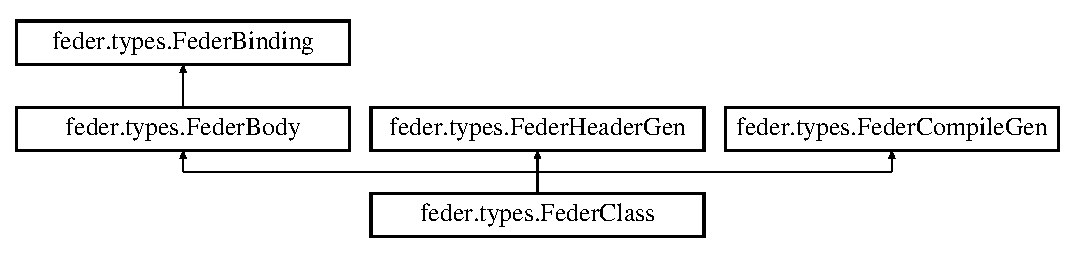
\includegraphics[height=2.947368cm]{classfeder_1_1types_1_1FederClass}
\end{center}
\end{figure}
\subsection*{Public Member Functions}
\begin{DoxyCompactItemize}
\item 
\hyperlink{classfeder_1_1types_1_1FederClass_a6599d0085106c898b54f1d0586e24931}{Feder\+Class} (\hyperlink{classfeder_1_1FederCompiler}{Feder\+Compiler} compiler0, String name0, \hyperlink{classfeder_1_1types_1_1FederBody}{Feder\+Body} parent0)
\item 
\hyperlink{classfeder_1_1types_1_1FederClass_a597983dcbbfd20a2cb51c8e77a010905}{Feder\+Class} (\hyperlink{classfeder_1_1FederCompiler}{Feder\+Compiler} compiler0, String name0, \hyperlink{classfeder_1_1types_1_1FederBody}{Feder\+Body} parent0, boolean istype0)
\item 
\hyperlink{classfeder_1_1types_1_1FederClass}{Feder\+Class} \hyperlink{classfeder_1_1types_1_1FederClass_a33ee88c8e95095a0b1b0e53f1429149f}{get\+Inherit\+Parent} ()
\item 
boolean \hyperlink{classfeder_1_1types_1_1FederClass_a6f23b3ce236b6d4568226e0d73f57601}{is\+Type} ()
\item 
void \hyperlink{classfeder_1_1types_1_1FederClass_abb3f629d1d752c6f6a207f12d2bc715e}{set\+Inherit\+Parent} (\hyperlink{classfeder_1_1types_1_1FederClass}{Feder\+Class} inherit\+\_\+parent0)
\item 
String \hyperlink{classfeder_1_1types_1_1FederClass_af8a297a2144969b497d053771c855088}{generate\+C\+Name} ()
\item 
String \hyperlink{classfeder_1_1types_1_1FederClass_a8cdb0ce97458df81ac91636799b5049f}{generate\+C\+Name\+Only} ()
\item 
String \hyperlink{classfeder_1_1types_1_1FederClass_a13b9740438b256dba8be6e63c8a1cc88}{generate\+In\+Header} ()
\item 
String \hyperlink{classfeder_1_1types_1_1FederClass_a4e57f61fe5a5c561e12af11da1e8f37b}{generate\+In\+Compile} ()
\end{DoxyCompactItemize}
\subsection*{Protected Member Functions}
\begin{DoxyCompactItemize}
\item 
\hyperlink{classfeder_1_1types_1_1FederBinding}{Feder\+Binding} \hyperlink{classfeder_1_1types_1_1FederClass_aa91ec183841e74c532a87ca8883cf782}{get\+Binding} (\hyperlink{classfeder_1_1types_1_1FederBody}{Feder\+Body} requestingbody, String name0, boolean allowparent, List$<$ \hyperlink{classfeder_1_1types_1_1FederBody}{Feder\+Body} $>$ bodies\+Checked)
\item 
\hyperlink{interfacefeder_1_1types_1_1FederArguments}{Feder\+Arguments} \hyperlink{classfeder_1_1types_1_1FederClass_a5863f07dc8fbadc8451439c50c9c8fd5}{get\+Function} (\hyperlink{classfeder_1_1types_1_1FederBody}{Feder\+Body} requestingbody, String name1, List$<$ \hyperlink{classfeder_1_1types_1_1FederBinding}{Feder\+Binding} $>$ arguments, boolean allow\+Parent, List$<$ \hyperlink{classfeder_1_1types_1_1FederBody}{Feder\+Body} $>$ bodies\+Checked)
\end{DoxyCompactItemize}
\subsection*{Additional Inherited Members}


\subsection{Detailed Description}
\begin{DoxyAuthor}{Author}
Fionn Langhans 
\end{DoxyAuthor}


\subsection{Constructor \& Destructor Documentation}
\mbox{\Hypertarget{classfeder_1_1types_1_1FederClass_a6599d0085106c898b54f1d0586e24931}\label{classfeder_1_1types_1_1FederClass_a6599d0085106c898b54f1d0586e24931}} 
\index{feder\+::types\+::\+Feder\+Class@{feder\+::types\+::\+Feder\+Class}!Feder\+Class@{Feder\+Class}}
\index{Feder\+Class@{Feder\+Class}!feder\+::types\+::\+Feder\+Class@{feder\+::types\+::\+Feder\+Class}}
\subsubsection{\texorpdfstring{Feder\+Class()}{FederClass()}\hspace{0.1cm}{\footnotesize\ttfamily [1/2]}}
{\footnotesize\ttfamily feder.\+types.\+Feder\+Class.\+Feder\+Class (\begin{DoxyParamCaption}\item[{\hyperlink{classfeder_1_1FederCompiler}{Feder\+Compiler}}]{compiler0,  }\item[{String}]{name0,  }\item[{\hyperlink{classfeder_1_1types_1_1FederBody}{Feder\+Body}}]{parent0 }\end{DoxyParamCaption})}


\begin{DoxyParams}{Parameters}
{\em compiler0} & The compiler instance to use \\
\hline
{\em name0} & The name/binding of the class/datatype \\
\hline
{\em parent0} & The parent of this body \\
\hline
\end{DoxyParams}
\mbox{\Hypertarget{classfeder_1_1types_1_1FederClass_a597983dcbbfd20a2cb51c8e77a010905}\label{classfeder_1_1types_1_1FederClass_a597983dcbbfd20a2cb51c8e77a010905}} 
\index{feder\+::types\+::\+Feder\+Class@{feder\+::types\+::\+Feder\+Class}!Feder\+Class@{Feder\+Class}}
\index{Feder\+Class@{Feder\+Class}!feder\+::types\+::\+Feder\+Class@{feder\+::types\+::\+Feder\+Class}}
\subsubsection{\texorpdfstring{Feder\+Class()}{FederClass()}\hspace{0.1cm}{\footnotesize\ttfamily [2/2]}}
{\footnotesize\ttfamily feder.\+types.\+Feder\+Class.\+Feder\+Class (\begin{DoxyParamCaption}\item[{\hyperlink{classfeder_1_1FederCompiler}{Feder\+Compiler}}]{compiler0,  }\item[{String}]{name0,  }\item[{\hyperlink{classfeder_1_1types_1_1FederBody}{Feder\+Body}}]{parent0,  }\item[{boolean}]{istype0 }\end{DoxyParamCaption})}


\begin{DoxyParams}{Parameters}
{\em compiler0} & The compiler instance to use \\
\hline
{\em name0} & The name/binding of the class/datatype \\
\hline
{\em parent0} & The parent of this body \\
\hline
{\em istype0} & Is type ? \\
\hline
\end{DoxyParams}


\subsection{Member Function Documentation}
\mbox{\Hypertarget{classfeder_1_1types_1_1FederClass_af8a297a2144969b497d053771c855088}\label{classfeder_1_1types_1_1FederClass_af8a297a2144969b497d053771c855088}} 
\index{feder\+::types\+::\+Feder\+Class@{feder\+::types\+::\+Feder\+Class}!generate\+C\+Name@{generate\+C\+Name}}
\index{generate\+C\+Name@{generate\+C\+Name}!feder\+::types\+::\+Feder\+Class@{feder\+::types\+::\+Feder\+Class}}
\subsubsection{\texorpdfstring{generate\+C\+Name()}{generateCName()}}
{\footnotesize\ttfamily String feder.\+types.\+Feder\+Class.\+generate\+C\+Name (\begin{DoxyParamCaption}{ }\end{DoxyParamCaption})}

\begin{DoxyReturn}{Returns}
Returns the name for the native language (C) 
\end{DoxyReturn}
\mbox{\Hypertarget{classfeder_1_1types_1_1FederClass_a8cdb0ce97458df81ac91636799b5049f}\label{classfeder_1_1types_1_1FederClass_a8cdb0ce97458df81ac91636799b5049f}} 
\index{feder\+::types\+::\+Feder\+Class@{feder\+::types\+::\+Feder\+Class}!generate\+C\+Name\+Only@{generate\+C\+Name\+Only}}
\index{generate\+C\+Name\+Only@{generate\+C\+Name\+Only}!feder\+::types\+::\+Feder\+Class@{feder\+::types\+::\+Feder\+Class}}
\subsubsection{\texorpdfstring{generate\+C\+Name\+Only()}{generateCNameOnly()}}
{\footnotesize\ttfamily String feder.\+types.\+Feder\+Class.\+generate\+C\+Name\+Only (\begin{DoxyParamCaption}{ }\end{DoxyParamCaption})}

\begin{DoxyReturn}{Returns}
Returns the name for the native language (C) without memory specifiers or anything like that 
\end{DoxyReturn}
\mbox{\Hypertarget{classfeder_1_1types_1_1FederClass_a4e57f61fe5a5c561e12af11da1e8f37b}\label{classfeder_1_1types_1_1FederClass_a4e57f61fe5a5c561e12af11da1e8f37b}} 
\index{feder\+::types\+::\+Feder\+Class@{feder\+::types\+::\+Feder\+Class}!generate\+In\+Compile@{generate\+In\+Compile}}
\index{generate\+In\+Compile@{generate\+In\+Compile}!feder\+::types\+::\+Feder\+Class@{feder\+::types\+::\+Feder\+Class}}
\subsubsection{\texorpdfstring{generate\+In\+Compile()}{generateInCompile()}}
{\footnotesize\ttfamily String feder.\+types.\+Feder\+Class.\+generate\+In\+Compile (\begin{DoxyParamCaption}{ }\end{DoxyParamCaption})}

\begin{DoxyReturn}{Returns}
Returns a string, which should be generated in the compile/code file. 
\end{DoxyReturn}


Implements \hyperlink{interfacefeder_1_1types_1_1FederCompileGen}{feder.\+types.\+Feder\+Compile\+Gen}.

\mbox{\Hypertarget{classfeder_1_1types_1_1FederClass_a13b9740438b256dba8be6e63c8a1cc88}\label{classfeder_1_1types_1_1FederClass_a13b9740438b256dba8be6e63c8a1cc88}} 
\index{feder\+::types\+::\+Feder\+Class@{feder\+::types\+::\+Feder\+Class}!generate\+In\+Header@{generate\+In\+Header}}
\index{generate\+In\+Header@{generate\+In\+Header}!feder\+::types\+::\+Feder\+Class@{feder\+::types\+::\+Feder\+Class}}
\subsubsection{\texorpdfstring{generate\+In\+Header()}{generateInHeader()}}
{\footnotesize\ttfamily String feder.\+types.\+Feder\+Class.\+generate\+In\+Header (\begin{DoxyParamCaption}{ }\end{DoxyParamCaption})}

\begin{DoxyReturn}{Returns}
Returns a string, which should be generated in the header file. 
\end{DoxyReturn}


Implements \hyperlink{interfacefeder_1_1types_1_1FederHeaderGen}{feder.\+types.\+Feder\+Header\+Gen}.

\mbox{\Hypertarget{classfeder_1_1types_1_1FederClass_aa91ec183841e74c532a87ca8883cf782}\label{classfeder_1_1types_1_1FederClass_aa91ec183841e74c532a87ca8883cf782}} 
\index{feder\+::types\+::\+Feder\+Class@{feder\+::types\+::\+Feder\+Class}!get\+Binding@{get\+Binding}}
\index{get\+Binding@{get\+Binding}!feder\+::types\+::\+Feder\+Class@{feder\+::types\+::\+Feder\+Class}}
\subsubsection{\texorpdfstring{get\+Binding()}{getBinding()}}
{\footnotesize\ttfamily \hyperlink{classfeder_1_1types_1_1FederBinding}{Feder\+Binding} feder.\+types.\+Feder\+Class.\+get\+Binding (\begin{DoxyParamCaption}\item[{\hyperlink{classfeder_1_1types_1_1FederBody}{Feder\+Body}}]{requestingbody,  }\item[{String}]{name0,  }\item[{boolean}]{allowparent,  }\item[{List$<$ \hyperlink{classfeder_1_1types_1_1FederBody}{Feder\+Body} $>$}]{bodies\+Checked }\end{DoxyParamCaption})\hspace{0.3cm}{\ttfamily [protected]}}


\begin{DoxyParams}{Parameters}
{\em requestingbody} & The body, which requests the binding \\
\hline
{\em name0} & the binding\textquotesingle{}s name \\
\hline
{\em allowparent} & Allow to search through parent (bodies) \\
\hline
{\em bodies\+Checked} & Race detection \\
\hline
\end{DoxyParams}
\begin{DoxyReturn}{Returns}
Returns a fitting binding. If nothing was found, null. 
\end{DoxyReturn}
\mbox{\Hypertarget{classfeder_1_1types_1_1FederClass_a5863f07dc8fbadc8451439c50c9c8fd5}\label{classfeder_1_1types_1_1FederClass_a5863f07dc8fbadc8451439c50c9c8fd5}} 
\index{feder\+::types\+::\+Feder\+Class@{feder\+::types\+::\+Feder\+Class}!get\+Function@{get\+Function}}
\index{get\+Function@{get\+Function}!feder\+::types\+::\+Feder\+Class@{feder\+::types\+::\+Feder\+Class}}
\subsubsection{\texorpdfstring{get\+Function()}{getFunction()}}
{\footnotesize\ttfamily \hyperlink{interfacefeder_1_1types_1_1FederArguments}{Feder\+Arguments} feder.\+types.\+Feder\+Class.\+get\+Function (\begin{DoxyParamCaption}\item[{\hyperlink{classfeder_1_1types_1_1FederBody}{Feder\+Body}}]{requestingbody,  }\item[{String}]{name1,  }\item[{List$<$ \hyperlink{classfeder_1_1types_1_1FederBinding}{Feder\+Binding} $>$}]{arguments,  }\item[{boolean}]{allow\+Parent,  }\item[{List$<$ \hyperlink{classfeder_1_1types_1_1FederBody}{Feder\+Body} $>$}]{bodies\+Checked }\end{DoxyParamCaption})\hspace{0.3cm}{\ttfamily [protected]}}


\begin{DoxyParams}{Parameters}
{\em requestingbody} & The body, which requests the binding \\
\hline
{\em name1} & The binding\textquotesingle{}s name \\
\hline
{\em arguments} & The arguments, which the function should have. \\
\hline
{\em allow\+Parent} & Allow to search through parents (bodies) \\
\hline
{\em bodies\+Checked} & Race detection \\
\hline
\end{DoxyParams}
\begin{DoxyReturn}{Returns}
Returns a fitting function name. If nothing was found, null. 
\end{DoxyReturn}
\mbox{\Hypertarget{classfeder_1_1types_1_1FederClass_a33ee88c8e95095a0b1b0e53f1429149f}\label{classfeder_1_1types_1_1FederClass_a33ee88c8e95095a0b1b0e53f1429149f}} 
\index{feder\+::types\+::\+Feder\+Class@{feder\+::types\+::\+Feder\+Class}!get\+Inherit\+Parent@{get\+Inherit\+Parent}}
\index{get\+Inherit\+Parent@{get\+Inherit\+Parent}!feder\+::types\+::\+Feder\+Class@{feder\+::types\+::\+Feder\+Class}}
\subsubsection{\texorpdfstring{get\+Inherit\+Parent()}{getInheritParent()}}
{\footnotesize\ttfamily \hyperlink{classfeder_1_1types_1_1FederClass}{Feder\+Class} feder.\+types.\+Feder\+Class.\+get\+Inherit\+Parent (\begin{DoxyParamCaption}{ }\end{DoxyParamCaption})}

\begin{DoxyReturn}{Returns}
Returns the parent \textquotesingle{}this class\textquotesingle{} inherits from (the class in \hyperlink{classfeder_1_1Feder}{Feder}) 
\end{DoxyReturn}
\mbox{\Hypertarget{classfeder_1_1types_1_1FederClass_a6f23b3ce236b6d4568226e0d73f57601}\label{classfeder_1_1types_1_1FederClass_a6f23b3ce236b6d4568226e0d73f57601}} 
\index{feder\+::types\+::\+Feder\+Class@{feder\+::types\+::\+Feder\+Class}!is\+Type@{is\+Type}}
\index{is\+Type@{is\+Type}!feder\+::types\+::\+Feder\+Class@{feder\+::types\+::\+Feder\+Class}}
\subsubsection{\texorpdfstring{is\+Type()}{isType()}}
{\footnotesize\ttfamily boolean feder.\+types.\+Feder\+Class.\+is\+Type (\begin{DoxyParamCaption}{ }\end{DoxyParamCaption})}

\begin{DoxyReturn}{Returns}
Returns true if this \textquotesingle{}class\textquotesingle{} is a datatype (declared with \textquotesingle{}type\textquotesingle{}) 
\end{DoxyReturn}
\mbox{\Hypertarget{classfeder_1_1types_1_1FederClass_abb3f629d1d752c6f6a207f12d2bc715e}\label{classfeder_1_1types_1_1FederClass_abb3f629d1d752c6f6a207f12d2bc715e}} 
\index{feder\+::types\+::\+Feder\+Class@{feder\+::types\+::\+Feder\+Class}!set\+Inherit\+Parent@{set\+Inherit\+Parent}}
\index{set\+Inherit\+Parent@{set\+Inherit\+Parent}!feder\+::types\+::\+Feder\+Class@{feder\+::types\+::\+Feder\+Class}}
\subsubsection{\texorpdfstring{set\+Inherit\+Parent()}{setInheritParent()}}
{\footnotesize\ttfamily void feder.\+types.\+Feder\+Class.\+set\+Inherit\+Parent (\begin{DoxyParamCaption}\item[{\hyperlink{classfeder_1_1types_1_1FederClass}{Feder\+Class}}]{inherit\+\_\+parent0 }\end{DoxyParamCaption})}

This method sets the inherited class of \textquotesingle{}this class\textquotesingle{}


\begin{DoxyParams}{Parameters}
{\em inherit\+\_\+parent0} & \\
\hline
\end{DoxyParams}


The documentation for this class was generated from the following file\+:\begin{DoxyCompactItemize}
\item 
src/feder/types/Feder\+Class.\+java\end{DoxyCompactItemize}

\hypertarget{interfacefeder_1_1types_1_1FederCompileGen}{}\section{feder.\+types.\+Feder\+Compile\+Gen Interface Reference}
\label{interfacefeder_1_1types_1_1FederCompileGen}\index{feder.\+types.\+Feder\+Compile\+Gen@{feder.\+types.\+Feder\+Compile\+Gen}}
Inheritance diagram for feder.\+types.\+Feder\+Compile\+Gen\+:\begin{figure}[H]
\begin{center}
\leavevmode
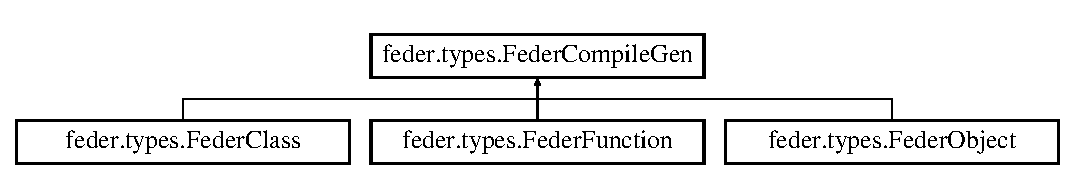
\includegraphics[height=1.964912cm]{interfacefeder_1_1types_1_1FederCompileGen}
\end{center}
\end{figure}
\subsection*{Public Member Functions}
\begin{DoxyCompactItemize}
\item 
\mbox{\Hypertarget{interfacefeder_1_1types_1_1FederCompileGen_ab952553ac05aa692aee4bead3268ba12}\label{interfacefeder_1_1types_1_1FederCompileGen_ab952553ac05aa692aee4bead3268ba12}} 
String {\bfseries generate\+In\+Compile} ()
\end{DoxyCompactItemize}


The documentation for this interface was generated from the following file\+:\begin{DoxyCompactItemize}
\item 
src/feder/types/Feder\+Compile\+Gen.\+java\end{DoxyCompactItemize}

\hypertarget{classfeder_1_1FederCompiler}{}\section{feder.\+Feder\+Compiler Class Reference}
\label{classfeder_1_1FederCompiler}\index{feder.\+Feder\+Compiler@{feder.\+Feder\+Compiler}}
\subsection*{Public Member Functions}
\begin{DoxyCompactItemize}
\item 
\mbox{\Hypertarget{classfeder_1_1FederCompiler_a1ed2c34c2f6ff52ca2a1d5e5bb79946a}\label{classfeder_1_1FederCompiler_a1ed2c34c2f6ff52ca2a1d5e5bb79946a}} 
{\bfseries Feder\+Compiler} (String name0, boolean debug0, String system\+Name, String prog\+C\+C0, boolean usewincl0, boolean nomultithread0, boolean print\+Commands0)
\item 
\hyperlink{classfeder_1_1FederCompiler_a8038b27d1ee4bdd165242833646f721c}{Feder\+Compiler} (String name0, \hyperlink{classfeder_1_1FederCompiler}{Feder\+Compiler} compiler)
\item 
\mbox{\Hypertarget{classfeder_1_1FederCompiler_a834ccd91bec2943484549f99ffabfd4c}\label{classfeder_1_1FederCompiler_a834ccd91bec2943484549f99ffabfd4c}} 
\hyperlink{classfeder_1_1types_1_1FederRule}{Feder\+Rule} {\bfseries get\+Apply\+Rule\+For} (String operator, \hyperlink{classfeder_1_1types_1_1FederBinding}{Feder\+Binding} lvalue, \hyperlink{classfeder_1_1types_1_1FederBinding}{Feder\+Binding} rvalue)
\item 
\mbox{\Hypertarget{classfeder_1_1FederCompiler_a18fd3fb928f7ac1ab8216fc26feb01cc}\label{classfeder_1_1FederCompiler_a18fd3fb928f7ac1ab8216fc26feb01cc}} 
\hyperlink{classfeder_1_1types_1_1FederRule}{Feder\+Rule} {\bfseries get\+Applyable\+Rule\+For\+Buildin} (String buildin\+\_\+name)
\item 
\mbox{\Hypertarget{classfeder_1_1FederCompiler_aa482c1a916e0cf8bf02fdd729be6d14c}\label{classfeder_1_1FederCompiler_aa482c1a916e0cf8bf02fdd729be6d14c}} 
\hyperlink{classfeder_1_1types_1_1FederRule}{Feder\+Rule} {\bfseries get\+Applyable\+Rule\+For\+Struct} (String buildin\+\_\+name)
\item 
\mbox{\Hypertarget{classfeder_1_1FederCompiler_a37e5e6ebae74b840de0a1697ce8a3d55}\label{classfeder_1_1FederCompiler_a37e5e6ebae74b840de0a1697ce8a3d55}} 
boolean {\bfseries is\+Debug} ()
\item 
String \hyperlink{classfeder_1_1FederCompiler_a4ae5a5159ac30049c08879dfca2fe308}{get\+Name} ()
\item 
String \hyperlink{classfeder_1_1FederCompiler_af56778dff690131320aaa2b7b8d1b8fb}{get\+Name\+File\+Header} ()
\item 
String \hyperlink{classfeder_1_1FederCompiler_ae130cb8cd6fa40d714dfa314d97243dd}{get\+Name\+File\+Header\+Only} ()
\item 
String \hyperlink{classfeder_1_1FederCompiler_a0cfbca0eeb6cccdb953d1f4232aba37e}{get\+Name\+File\+Compile} ()
\item 
String \hyperlink{classfeder_1_1FederCompiler_a01b3fa2b74ccce828f5afa1792d2b4a0}{get\+Name\+File\+Compile\+Only} ()
\item 
String \hyperlink{classfeder_1_1FederCompiler_a1c4f7b541e25baae015492afcbb96965}{get\+Name\+File\+Object} ()
\item 
\mbox{\Hypertarget{classfeder_1_1FederCompiler_ac798ce8c56d635322cc10a64a4ba9235}\label{classfeder_1_1FederCompiler_ac798ce8c56d635322cc10a64a4ba9235}} 
String {\bfseries get\+Name\+File\+Object\+Only} ()
\item 
boolean \hyperlink{classfeder_1_1FederCompiler_a33c8a6aab78bef99df17306c9a3e9c95}{already\+Included} (String name0)
\item 
void \hyperlink{classfeder_1_1FederCompiler_aac12b9b09fb8a5a0caaf62e021bbeae7}{add\+Macros} (List$<$ String $>$ macros)
\item 
\hyperlink{classfeder_1_1FederCompiler}{Feder\+Compiler} \hyperlink{classfeder_1_1FederCompiler_a84f29a6bcfa849ab97b0aed77e1008c3}{get\+Compiler} (String name0)
\item 
\hyperlink{classfeder_1_1types_1_1FederNamespace}{Feder\+Namespace} \hyperlink{classfeder_1_1FederCompiler_adfef64d211b87229b254e05144d00caf}{compile} (String text0)
\item 
String \hyperlink{classfeder_1_1FederCompiler_ab3314b260330e1ce37132849bcb50b75}{generate\+Library\+Caller\+Function\+Name} ()
\item 
\mbox{\Hypertarget{classfeder_1_1FederCompiler_af2cb36b66498704682c6b3eb4ea99f63}\label{classfeder_1_1FederCompiler_af2cb36b66498704682c6b3eb4ea99f63}} 
void {\bfseries write\+To\+File\+Forward\+Declaration} (Buffered\+Writer header\+File)  throws I\+O\+Exception 	
\item 
void \hyperlink{classfeder_1_1FederCompiler_a4e72abbcf700edf0f31ce2aea2605cb9}{write\+To\+File} (Buffered\+Writer compile\+File, Buffered\+Writer header\+File, \hyperlink{classfeder_1_1types_1_1FederBinding}{Feder\+Binding} body1)  throws I\+O\+Exception 	
\item 
void \hyperlink{classfeder_1_1FederCompiler_a11c62c5eaf76b4a8e1b994981cb88ff3}{inform\+Include} (String name1)
\end{DoxyCompactItemize}
\subsection*{Public Attributes}
\begin{DoxyCompactItemize}
\item 
boolean \hyperlink{classfeder_1_1FederCompiler_a5ee5791f203fe9785e84558b0ca1eb51}{allow\+Main} = true
\item 
boolean \hyperlink{classfeder_1_1FederCompiler_aa2d3d96c99a1a600acdcdc5c0fc3910e}{usewincl} = false
\item 
String \hyperlink{classfeder_1_1FederCompiler_a6bd58a0bde5e940c88c2865bf64bebd8}{build\+Dir} = \char`\"{}./\char`\"{}
\item 
List$<$ String $>$ \hyperlink{classfeder_1_1FederCompiler_a38f7cfc41d820998a340814766d251c3}{include\+Dirs} = new Linked\+List$<$String$>$()
\item 
List$<$ \hyperlink{classfeder_1_1FederCompiler}{Feder\+Compiler} $>$ \hyperlink{classfeder_1_1FederCompiler_a4509ee4224d7822411d242ae342a316e}{included} = new Linked\+List$<$$>$()
\item 
List$<$ \hyperlink{classfeder_1_1FederCompiler}{Feder\+Compiler} $>$ \hyperlink{classfeder_1_1FederCompiler_abc41d1f375e7b851bc3967833650ec7b}{global\+Included} = new Linked\+List$<$$>$()
\item 
List$<$ \hyperlink{classfeder_1_1types_1_1FederBinding}{Feder\+Binding} $>$ \hyperlink{classfeder_1_1FederCompiler_ab971df77c967493bc7aa312233aeb24a}{build\+Order} = new Linked\+List$<$$>$()
\item 
boolean \hyperlink{classfeder_1_1FederCompiler_a41515b8539e22e6899993b574a10e203}{allow\+C\+Ccompile} = true
\item 
String \hyperlink{classfeder_1_1FederCompiler_a00a0ae826fb482e7c2c1ecbfde051218}{prog\+CC} = \char`\"{}cc\char`\"{}
\item 
List$<$ String $>$ \hyperlink{classfeder_1_1FederCompiler_a59d4d26003b722044c7d36a09c2c36e8}{prog\+C\+C\+Options} = new Linked\+List$<$$>$()
\item 
List$<$ String $>$ \hyperlink{classfeder_1_1FederCompiler_a71296ee1ff3cf6efff0bafb76b2e7f4c}{linker\+Options} = new Linked\+List$<$$>$()
\item 
\mbox{\Hypertarget{classfeder_1_1FederCompiler_a448b8b53998b4607ae197ede3ef4310f}\label{classfeder_1_1FederCompiler_a448b8b53998b4607ae197ede3ef4310f}} 
boolean {\bfseries print\+Commands} = false
\item 
\hyperlink{classfeder_1_1types_1_1FederNamespace}{Feder\+Namespace} \hyperlink{classfeder_1_1FederCompiler_ae1ddfe80b0facbe91b5d0d9ab62882a5}{main}
\item 
\mbox{\Hypertarget{classfeder_1_1FederCompiler_ab0331eb16d237f2d9cf60dba4e8b3cff}\label{classfeder_1_1FederCompiler_ab0331eb16d237f2d9cf60dba4e8b3cff}} 
boolean {\bfseries preprocessor\+Was\+True} = false
\item 
\mbox{\Hypertarget{classfeder_1_1FederCompiler_a2d5a51b073a7fdd2f5466b0981c91c25}\label{classfeder_1_1FederCompiler_a2d5a51b073a7fdd2f5466b0981c91c25}} 
boolean {\bfseries preprocessor\+Skip\+Code} = false
\item 
\mbox{\Hypertarget{classfeder_1_1FederCompiler_a2c22544bd964e7754f64b3b3b4161d2a}\label{classfeder_1_1FederCompiler_a2c22544bd964e7754f64b3b3b4161d2a}} 
boolean {\bfseries preprocessor\+If\+Came} = false
\item 
\mbox{\Hypertarget{classfeder_1_1FederCompiler_a47a2494cf67ceea55cd84be8b50f2483}\label{classfeder_1_1FederCompiler_a47a2494cf67ceea55cd84be8b50f2483}} 
List$<$ String $>$ {\bfseries preprocessor\+Macros} = new Linked\+List$<$$>$()
\item 
List$<$ \hyperlink{classfeder_1_1types_1_1FederRule}{Feder\+Rule} $>$ \hyperlink{classfeder_1_1FederCompiler_ae1a246f2474872537f0ac3ad3bc6dd79}{feder\+\_\+rules} = new Linked\+List$<$$>$()
\item 
\mbox{\Hypertarget{classfeder_1_1FederCompiler_a4bafca1a1bbbb03f1d30dc38d8aff83e}\label{classfeder_1_1FederCompiler_a4bafca1a1bbbb03f1d30dc38d8aff83e}} 
boolean {\bfseries fatal\+Error} = false
\end{DoxyCompactItemize}


\subsection{Detailed Description}
\begin{DoxyAuthor}{Author}
Fionn Langhans 
\end{DoxyAuthor}


\subsection{Constructor \& Destructor Documentation}
\mbox{\Hypertarget{classfeder_1_1FederCompiler_a8038b27d1ee4bdd165242833646f721c}\label{classfeder_1_1FederCompiler_a8038b27d1ee4bdd165242833646f721c}} 
\index{feder\+::\+Feder\+Compiler@{feder\+::\+Feder\+Compiler}!Feder\+Compiler@{Feder\+Compiler}}
\index{Feder\+Compiler@{Feder\+Compiler}!feder\+::\+Feder\+Compiler@{feder\+::\+Feder\+Compiler}}
\subsubsection{\texorpdfstring{Feder\+Compiler()}{FederCompiler()}}
{\footnotesize\ttfamily feder.\+Feder\+Compiler.\+Feder\+Compiler (\begin{DoxyParamCaption}\item[{String}]{name0,  }\item[{\hyperlink{classfeder_1_1FederCompiler}{Feder\+Compiler}}]{compiler }\end{DoxyParamCaption})}

Create a compiler, which depends on an other compiler 

\subsection{Member Function Documentation}
\mbox{\Hypertarget{classfeder_1_1FederCompiler_aac12b9b09fb8a5a0caaf62e021bbeae7}\label{classfeder_1_1FederCompiler_aac12b9b09fb8a5a0caaf62e021bbeae7}} 
\index{feder\+::\+Feder\+Compiler@{feder\+::\+Feder\+Compiler}!add\+Macros@{add\+Macros}}
\index{add\+Macros@{add\+Macros}!feder\+::\+Feder\+Compiler@{feder\+::\+Feder\+Compiler}}
\subsubsection{\texorpdfstring{add\+Macros()}{addMacros()}}
{\footnotesize\ttfamily void feder.\+Feder\+Compiler.\+add\+Macros (\begin{DoxyParamCaption}\item[{List$<$ String $>$}]{macros }\end{DoxyParamCaption})}

Add a preprocessor macro to preprocessor\+Macros \mbox{\Hypertarget{classfeder_1_1FederCompiler_a33c8a6aab78bef99df17306c9a3e9c95}\label{classfeder_1_1FederCompiler_a33c8a6aab78bef99df17306c9a3e9c95}} 
\index{feder\+::\+Feder\+Compiler@{feder\+::\+Feder\+Compiler}!already\+Included@{already\+Included}}
\index{already\+Included@{already\+Included}!feder\+::\+Feder\+Compiler@{feder\+::\+Feder\+Compiler}}
\subsubsection{\texorpdfstring{already\+Included()}{alreadyIncluded()}}
{\footnotesize\ttfamily boolean feder.\+Feder\+Compiler.\+already\+Included (\begin{DoxyParamCaption}\item[{String}]{name0 }\end{DoxyParamCaption})}

\begin{DoxyReturn}{Returns}
Returns true, if the include file named \textquotesingle{}name0\textquotesingle{} has already been included once in the current file (compiler) 
\end{DoxyReturn}
\mbox{\Hypertarget{classfeder_1_1FederCompiler_adfef64d211b87229b254e05144d00caf}\label{classfeder_1_1FederCompiler_adfef64d211b87229b254e05144d00caf}} 
\index{feder\+::\+Feder\+Compiler@{feder\+::\+Feder\+Compiler}!compile@{compile}}
\index{compile@{compile}!feder\+::\+Feder\+Compiler@{feder\+::\+Feder\+Compiler}}
\subsubsection{\texorpdfstring{compile()}{compile()}}
{\footnotesize\ttfamily \hyperlink{classfeder_1_1types_1_1FederNamespace}{Feder\+Namespace} feder.\+Feder\+Compiler.\+compile (\begin{DoxyParamCaption}\item[{String}]{text0 }\end{DoxyParamCaption})}

This function compiles the given \textquotesingle{}text0\textquotesingle{}. This means this method first converts the \hyperlink{classfeder_1_1Feder}{Feder} source code to C source code. After that step and if all has been successfully, this method will compile the generated C files with a given C compiler (if allowcccompiler is true). 
\begin{DoxyParams}{Parameters}
{\em text0} & \hyperlink{classfeder_1_1Feder}{Feder} source code \\
\hline
\end{DoxyParams}
\begin{DoxyReturn}{Returns}
Returns the \textquotesingle{}genisis\textquotesingle{} namespace. 
\end{DoxyReturn}
If this value is greater than 0, the compiler will return an error code

A new line has been started

The following inserts code, which changes the args given the program to a \hyperlink{classfeder_1_1Feder}{Feder} compatible object (fdc\+\_\+\+List)\mbox{\Hypertarget{classfeder_1_1FederCompiler_ab3314b260330e1ce37132849bcb50b75}\label{classfeder_1_1FederCompiler_ab3314b260330e1ce37132849bcb50b75}} 
\index{feder\+::\+Feder\+Compiler@{feder\+::\+Feder\+Compiler}!generate\+Library\+Caller\+Function\+Name@{generate\+Library\+Caller\+Function\+Name}}
\index{generate\+Library\+Caller\+Function\+Name@{generate\+Library\+Caller\+Function\+Name}!feder\+::\+Feder\+Compiler@{feder\+::\+Feder\+Compiler}}
\subsubsection{\texorpdfstring{generate\+Library\+Caller\+Function\+Name()}{generateLibraryCallerFunctionName()}}
{\footnotesize\ttfamily String feder.\+Feder\+Compiler.\+generate\+Library\+Caller\+Function\+Name (\begin{DoxyParamCaption}{ }\end{DoxyParamCaption})}

Generate the name of the library load function \mbox{\Hypertarget{classfeder_1_1FederCompiler_a84f29a6bcfa849ab97b0aed77e1008c3}\label{classfeder_1_1FederCompiler_a84f29a6bcfa849ab97b0aed77e1008c3}} 
\index{feder\+::\+Feder\+Compiler@{feder\+::\+Feder\+Compiler}!get\+Compiler@{get\+Compiler}}
\index{get\+Compiler@{get\+Compiler}!feder\+::\+Feder\+Compiler@{feder\+::\+Feder\+Compiler}}
\subsubsection{\texorpdfstring{get\+Compiler()}{getCompiler()}}
{\footnotesize\ttfamily \hyperlink{classfeder_1_1FederCompiler}{Feder\+Compiler} feder.\+Feder\+Compiler.\+get\+Compiler (\begin{DoxyParamCaption}\item[{String}]{name0 }\end{DoxyParamCaption})}

\begin{DoxyReturn}{Returns}
Returns the compiler, which is named \textquotesingle{}name0\textquotesingle{}. If no compiler named \textquotesingle{}name0\textquotesingle{} has been found, this method returns \textquotesingle{}null\textquotesingle{}. 
\end{DoxyReturn}
\mbox{\Hypertarget{classfeder_1_1FederCompiler_a4ae5a5159ac30049c08879dfca2fe308}\label{classfeder_1_1FederCompiler_a4ae5a5159ac30049c08879dfca2fe308}} 
\index{feder\+::\+Feder\+Compiler@{feder\+::\+Feder\+Compiler}!get\+Name@{get\+Name}}
\index{get\+Name@{get\+Name}!feder\+::\+Feder\+Compiler@{feder\+::\+Feder\+Compiler}}
\subsubsection{\texorpdfstring{get\+Name()}{getName()}}
{\footnotesize\ttfamily String feder.\+Feder\+Compiler.\+get\+Name (\begin{DoxyParamCaption}{ }\end{DoxyParamCaption})}

Return the name of the current compiler, which was generated from the file name \mbox{\Hypertarget{classfeder_1_1FederCompiler_a0cfbca0eeb6cccdb953d1f4232aba37e}\label{classfeder_1_1FederCompiler_a0cfbca0eeb6cccdb953d1f4232aba37e}} 
\index{feder\+::\+Feder\+Compiler@{feder\+::\+Feder\+Compiler}!get\+Name\+File\+Compile@{get\+Name\+File\+Compile}}
\index{get\+Name\+File\+Compile@{get\+Name\+File\+Compile}!feder\+::\+Feder\+Compiler@{feder\+::\+Feder\+Compiler}}
\subsubsection{\texorpdfstring{get\+Name\+File\+Compile()}{getNameFileCompile()}}
{\footnotesize\ttfamily String feder.\+Feder\+Compiler.\+get\+Name\+File\+Compile (\begin{DoxyParamCaption}{ }\end{DoxyParamCaption})}

\begin{DoxyReturn}{Returns}
Returns the path to the source code file 
\end{DoxyReturn}
\mbox{\Hypertarget{classfeder_1_1FederCompiler_a01b3fa2b74ccce828f5afa1792d2b4a0}\label{classfeder_1_1FederCompiler_a01b3fa2b74ccce828f5afa1792d2b4a0}} 
\index{feder\+::\+Feder\+Compiler@{feder\+::\+Feder\+Compiler}!get\+Name\+File\+Compile\+Only@{get\+Name\+File\+Compile\+Only}}
\index{get\+Name\+File\+Compile\+Only@{get\+Name\+File\+Compile\+Only}!feder\+::\+Feder\+Compiler@{feder\+::\+Feder\+Compiler}}
\subsubsection{\texorpdfstring{get\+Name\+File\+Compile\+Only()}{getNameFileCompileOnly()}}
{\footnotesize\ttfamily String feder.\+Feder\+Compiler.\+get\+Name\+File\+Compile\+Only (\begin{DoxyParamCaption}{ }\end{DoxyParamCaption})}

\begin{DoxyReturn}{Returns}
Returns the name of the source code file, which is generated by the \textquotesingle{}compile\textquotesingle{} method. 
\end{DoxyReturn}
\mbox{\Hypertarget{classfeder_1_1FederCompiler_af56778dff690131320aaa2b7b8d1b8fb}\label{classfeder_1_1FederCompiler_af56778dff690131320aaa2b7b8d1b8fb}} 
\index{feder\+::\+Feder\+Compiler@{feder\+::\+Feder\+Compiler}!get\+Name\+File\+Header@{get\+Name\+File\+Header}}
\index{get\+Name\+File\+Header@{get\+Name\+File\+Header}!feder\+::\+Feder\+Compiler@{feder\+::\+Feder\+Compiler}}
\subsubsection{\texorpdfstring{get\+Name\+File\+Header()}{getNameFileHeader()}}
{\footnotesize\ttfamily String feder.\+Feder\+Compiler.\+get\+Name\+File\+Header (\begin{DoxyParamCaption}{ }\end{DoxyParamCaption})}

\begin{DoxyReturn}{Returns}
Returns the path to the header file, which will be generated by the \textquotesingle{}compile\textquotesingle{} method 
\end{DoxyReturn}
\mbox{\Hypertarget{classfeder_1_1FederCompiler_ae130cb8cd6fa40d714dfa314d97243dd}\label{classfeder_1_1FederCompiler_ae130cb8cd6fa40d714dfa314d97243dd}} 
\index{feder\+::\+Feder\+Compiler@{feder\+::\+Feder\+Compiler}!get\+Name\+File\+Header\+Only@{get\+Name\+File\+Header\+Only}}
\index{get\+Name\+File\+Header\+Only@{get\+Name\+File\+Header\+Only}!feder\+::\+Feder\+Compiler@{feder\+::\+Feder\+Compiler}}
\subsubsection{\texorpdfstring{get\+Name\+File\+Header\+Only()}{getNameFileHeaderOnly()}}
{\footnotesize\ttfamily String feder.\+Feder\+Compiler.\+get\+Name\+File\+Header\+Only (\begin{DoxyParamCaption}{ }\end{DoxyParamCaption})}

\begin{DoxyReturn}{Returns}
Returns the only the name of the header file. 
\end{DoxyReturn}
\mbox{\Hypertarget{classfeder_1_1FederCompiler_a1c4f7b541e25baae015492afcbb96965}\label{classfeder_1_1FederCompiler_a1c4f7b541e25baae015492afcbb96965}} 
\index{feder\+::\+Feder\+Compiler@{feder\+::\+Feder\+Compiler}!get\+Name\+File\+Object@{get\+Name\+File\+Object}}
\index{get\+Name\+File\+Object@{get\+Name\+File\+Object}!feder\+::\+Feder\+Compiler@{feder\+::\+Feder\+Compiler}}
\subsubsection{\texorpdfstring{get\+Name\+File\+Object()}{getNameFileObject()}}
{\footnotesize\ttfamily String feder.\+Feder\+Compiler.\+get\+Name\+File\+Object (\begin{DoxyParamCaption}{ }\end{DoxyParamCaption})}

\begin{DoxyReturn}{Returns}
Returns the path to the object file, which will be generated by the \textquotesingle{}compile\textquotesingle{} method, if the cc compiler is enabled. 
\end{DoxyReturn}
\mbox{\Hypertarget{classfeder_1_1FederCompiler_a11c62c5eaf76b4a8e1b994981cb88ff3}\label{classfeder_1_1FederCompiler_a11c62c5eaf76b4a8e1b994981cb88ff3}} 
\index{feder\+::\+Feder\+Compiler@{feder\+::\+Feder\+Compiler}!inform\+Include@{inform\+Include}}
\index{inform\+Include@{inform\+Include}!feder\+::\+Feder\+Compiler@{feder\+::\+Feder\+Compiler}}
\subsubsection{\texorpdfstring{inform\+Include()}{informInclude()}}
{\footnotesize\ttfamily void feder.\+Feder\+Compiler.\+inform\+Include (\begin{DoxyParamCaption}\item[{String}]{name1 }\end{DoxyParamCaption})}

This method tries to set the type of \char`\"{}args\char`\"{} to List, whenever possible \mbox{\Hypertarget{classfeder_1_1FederCompiler_a4e72abbcf700edf0f31ce2aea2605cb9}\label{classfeder_1_1FederCompiler_a4e72abbcf700edf0f31ce2aea2605cb9}} 
\index{feder\+::\+Feder\+Compiler@{feder\+::\+Feder\+Compiler}!write\+To\+File@{write\+To\+File}}
\index{write\+To\+File@{write\+To\+File}!feder\+::\+Feder\+Compiler@{feder\+::\+Feder\+Compiler}}
\subsubsection{\texorpdfstring{write\+To\+File()}{writeToFile()}}
{\footnotesize\ttfamily void feder.\+Feder\+Compiler.\+write\+To\+File (\begin{DoxyParamCaption}\item[{Buffered\+Writer}]{compile\+File,  }\item[{Buffered\+Writer}]{header\+File,  }\item[{\hyperlink{classfeder_1_1types_1_1FederBinding}{Feder\+Binding}}]{body1 }\end{DoxyParamCaption}) throws I\+O\+Exception}

Write the main code of the generated bodies to the files 

\subsection{Member Data Documentation}
\mbox{\Hypertarget{classfeder_1_1FederCompiler_a41515b8539e22e6899993b574a10e203}\label{classfeder_1_1FederCompiler_a41515b8539e22e6899993b574a10e203}} 
\index{feder\+::\+Feder\+Compiler@{feder\+::\+Feder\+Compiler}!allow\+C\+Ccompile@{allow\+C\+Ccompile}}
\index{allow\+C\+Ccompile@{allow\+C\+Ccompile}!feder\+::\+Feder\+Compiler@{feder\+::\+Feder\+Compiler}}
\subsubsection{\texorpdfstring{allow\+C\+Ccompile}{allowCCcompile}}
{\footnotesize\ttfamily boolean feder.\+Feder\+Compiler.\+allow\+C\+Ccompile = true}

This allows this program to start a cc compiler to generate an object file \mbox{\Hypertarget{classfeder_1_1FederCompiler_a5ee5791f203fe9785e84558b0ca1eb51}\label{classfeder_1_1FederCompiler_a5ee5791f203fe9785e84558b0ca1eb51}} 
\index{feder\+::\+Feder\+Compiler@{feder\+::\+Feder\+Compiler}!allow\+Main@{allow\+Main}}
\index{allow\+Main@{allow\+Main}!feder\+::\+Feder\+Compiler@{feder\+::\+Feder\+Compiler}}
\subsubsection{\texorpdfstring{allow\+Main}{allowMain}}
{\footnotesize\ttfamily boolean feder.\+Feder\+Compiler.\+allow\+Main = true}

Allows this compiler instance to generate \textquotesingle{}int main (int lenargs, char $\ast$$\ast$ vargs)\textquotesingle{} instead of the library loader function \mbox{\Hypertarget{classfeder_1_1FederCompiler_a6bd58a0bde5e940c88c2865bf64bebd8}\label{classfeder_1_1FederCompiler_a6bd58a0bde5e940c88c2865bf64bebd8}} 
\index{feder\+::\+Feder\+Compiler@{feder\+::\+Feder\+Compiler}!build\+Dir@{build\+Dir}}
\index{build\+Dir@{build\+Dir}!feder\+::\+Feder\+Compiler@{feder\+::\+Feder\+Compiler}}
\subsubsection{\texorpdfstring{build\+Dir}{buildDir}}
{\footnotesize\ttfamily String feder.\+Feder\+Compiler.\+build\+Dir = \char`\"{}./\char`\"{}}

The build directory, where the files should be generated \mbox{\Hypertarget{classfeder_1_1FederCompiler_ab971df77c967493bc7aa312233aeb24a}\label{classfeder_1_1FederCompiler_ab971df77c967493bc7aa312233aeb24a}} 
\index{feder\+::\+Feder\+Compiler@{feder\+::\+Feder\+Compiler}!build\+Order@{build\+Order}}
\index{build\+Order@{build\+Order}!feder\+::\+Feder\+Compiler@{feder\+::\+Feder\+Compiler}}
\subsubsection{\texorpdfstring{build\+Order}{buildOrder}}
{\footnotesize\ttfamily List$<$\hyperlink{classfeder_1_1types_1_1FederBinding}{Feder\+Binding}$>$ feder.\+Feder\+Compiler.\+build\+Order = new Linked\+List$<$$>$()}

This list represents, in which order the components should be build \mbox{\Hypertarget{classfeder_1_1FederCompiler_ae1a246f2474872537f0ac3ad3bc6dd79}\label{classfeder_1_1FederCompiler_ae1a246f2474872537f0ac3ad3bc6dd79}} 
\index{feder\+::\+Feder\+Compiler@{feder\+::\+Feder\+Compiler}!feder\+\_\+rules@{feder\+\_\+rules}}
\index{feder\+\_\+rules@{feder\+\_\+rules}!feder\+::\+Feder\+Compiler@{feder\+::\+Feder\+Compiler}}
\subsubsection{\texorpdfstring{feder\+\_\+rules}{feder\_rules}}
{\footnotesize\ttfamily List$<$\hyperlink{classfeder_1_1types_1_1FederRule}{Feder\+Rule}$>$ feder.\+Feder\+Compiler.\+feder\+\_\+rules = new Linked\+List$<$$>$()}

\hyperlink{classfeder_1_1Feder}{Feder} Rules ... \mbox{\Hypertarget{classfeder_1_1FederCompiler_abc41d1f375e7b851bc3967833650ec7b}\label{classfeder_1_1FederCompiler_abc41d1f375e7b851bc3967833650ec7b}} 
\index{feder\+::\+Feder\+Compiler@{feder\+::\+Feder\+Compiler}!global\+Included@{global\+Included}}
\index{global\+Included@{global\+Included}!feder\+::\+Feder\+Compiler@{feder\+::\+Feder\+Compiler}}
\subsubsection{\texorpdfstring{global\+Included}{globalIncluded}}
{\footnotesize\ttfamily List$<$\hyperlink{classfeder_1_1FederCompiler}{Feder\+Compiler}$>$ feder.\+Feder\+Compiler.\+global\+Included = new Linked\+List$<$$>$()}

This list contains compiler instances, which are generally used by the compile process \mbox{\Hypertarget{classfeder_1_1FederCompiler_a4509ee4224d7822411d242ae342a316e}\label{classfeder_1_1FederCompiler_a4509ee4224d7822411d242ae342a316e}} 
\index{feder\+::\+Feder\+Compiler@{feder\+::\+Feder\+Compiler}!included@{included}}
\index{included@{included}!feder\+::\+Feder\+Compiler@{feder\+::\+Feder\+Compiler}}
\subsubsection{\texorpdfstring{included}{included}}
{\footnotesize\ttfamily List$<$\hyperlink{classfeder_1_1FederCompiler}{Feder\+Compiler}$>$ feder.\+Feder\+Compiler.\+included = new Linked\+List$<$$>$()}

This list contains compiler instances, which are included by this compiler instance \mbox{\Hypertarget{classfeder_1_1FederCompiler_a38f7cfc41d820998a340814766d251c3}\label{classfeder_1_1FederCompiler_a38f7cfc41d820998a340814766d251c3}} 
\index{feder\+::\+Feder\+Compiler@{feder\+::\+Feder\+Compiler}!include\+Dirs@{include\+Dirs}}
\index{include\+Dirs@{include\+Dirs}!feder\+::\+Feder\+Compiler@{feder\+::\+Feder\+Compiler}}
\subsubsection{\texorpdfstring{include\+Dirs}{includeDirs}}
{\footnotesize\ttfamily List$<$String$>$ feder.\+Feder\+Compiler.\+include\+Dirs = new Linked\+List$<$String$>$()}

Which include directories should be used \mbox{\Hypertarget{classfeder_1_1FederCompiler_a71296ee1ff3cf6efff0bafb76b2e7f4c}\label{classfeder_1_1FederCompiler_a71296ee1ff3cf6efff0bafb76b2e7f4c}} 
\index{feder\+::\+Feder\+Compiler@{feder\+::\+Feder\+Compiler}!linker\+Options@{linker\+Options}}
\index{linker\+Options@{linker\+Options}!feder\+::\+Feder\+Compiler@{feder\+::\+Feder\+Compiler}}
\subsubsection{\texorpdfstring{linker\+Options}{linkerOptions}}
{\footnotesize\ttfamily List$<$String$>$ feder.\+Feder\+Compiler.\+linker\+Options = new Linked\+List$<$$>$()}

The list of options, which should be given to the linker (--loption) \mbox{\Hypertarget{classfeder_1_1FederCompiler_ae1ddfe80b0facbe91b5d0d9ab62882a5}\label{classfeder_1_1FederCompiler_ae1ddfe80b0facbe91b5d0d9ab62882a5}} 
\index{feder\+::\+Feder\+Compiler@{feder\+::\+Feder\+Compiler}!main@{main}}
\index{main@{main}!feder\+::\+Feder\+Compiler@{feder\+::\+Feder\+Compiler}}
\subsubsection{\texorpdfstring{main}{main}}
{\footnotesize\ttfamily \hyperlink{classfeder_1_1types_1_1FederNamespace}{Feder\+Namespace} feder.\+Feder\+Compiler.\+main}

This object is the main namespace of this compiler instance \mbox{\Hypertarget{classfeder_1_1FederCompiler_a00a0ae826fb482e7c2c1ecbfde051218}\label{classfeder_1_1FederCompiler_a00a0ae826fb482e7c2c1ecbfde051218}} 
\index{feder\+::\+Feder\+Compiler@{feder\+::\+Feder\+Compiler}!prog\+CC@{prog\+CC}}
\index{prog\+CC@{prog\+CC}!feder\+::\+Feder\+Compiler@{feder\+::\+Feder\+Compiler}}
\subsubsection{\texorpdfstring{prog\+CC}{progCC}}
{\footnotesize\ttfamily String feder.\+Feder\+Compiler.\+prog\+CC = \char`\"{}cc\char`\"{}}

The name of the cc compiler \mbox{\Hypertarget{classfeder_1_1FederCompiler_a59d4d26003b722044c7d36a09c2c36e8}\label{classfeder_1_1FederCompiler_a59d4d26003b722044c7d36a09c2c36e8}} 
\index{feder\+::\+Feder\+Compiler@{feder\+::\+Feder\+Compiler}!prog\+C\+C\+Options@{prog\+C\+C\+Options}}
\index{prog\+C\+C\+Options@{prog\+C\+C\+Options}!feder\+::\+Feder\+Compiler@{feder\+::\+Feder\+Compiler}}
\subsubsection{\texorpdfstring{prog\+C\+C\+Options}{progCCOptions}}
{\footnotesize\ttfamily List$<$String$>$ feder.\+Feder\+Compiler.\+prog\+C\+C\+Options = new Linked\+List$<$$>$()}

The list of options, which should be given to the cc compiler (--coption) \mbox{\Hypertarget{classfeder_1_1FederCompiler_aa2d3d96c99a1a600acdcdc5c0fc3910e}\label{classfeder_1_1FederCompiler_aa2d3d96c99a1a600acdcdc5c0fc3910e}} 
\index{feder\+::\+Feder\+Compiler@{feder\+::\+Feder\+Compiler}!usewincl@{usewincl}}
\index{usewincl@{usewincl}!feder\+::\+Feder\+Compiler@{feder\+::\+Feder\+Compiler}}
\subsubsection{\texorpdfstring{usewincl}{usewincl}}
{\footnotesize\ttfamily boolean feder.\+Feder\+Compiler.\+usewincl = false}

This value allows this program to use options for the visual studio c/c++ compiler instead of the ones for the G\+NU G\+CC compiler (or clang) 

The documentation for this class was generated from the following file\+:\begin{DoxyCompactItemize}
\item 
src/feder/Feder\+Compiler.\+java\end{DoxyCompactItemize}

\hypertarget{classfeder_1_1types_1_1FederFunction}{}\section{feder.\+types.\+Feder\+Function Class Reference}
\label{classfeder_1_1types_1_1FederFunction}\index{feder.\+types.\+Feder\+Function@{feder.\+types.\+Feder\+Function}}
Inheritance diagram for feder.\+types.\+Feder\+Function\+:\begin{figure}[H]
\begin{center}
\leavevmode
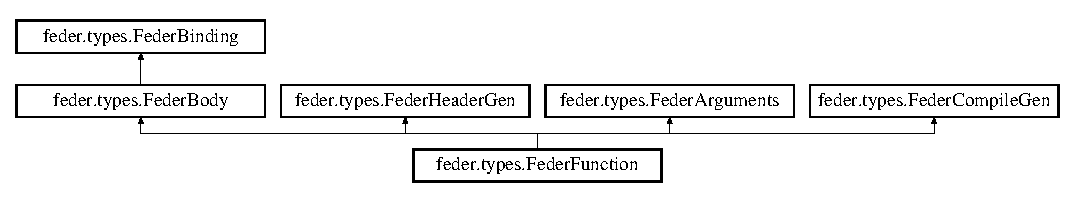
\includegraphics[height=2.210526cm]{classfeder_1_1types_1_1FederFunction}
\end{center}
\end{figure}
\subsection*{Public Member Functions}
\begin{DoxyCompactItemize}
\item 
\mbox{\Hypertarget{classfeder_1_1types_1_1FederFunction_a9e4e3582788c32d28af8b136e55ef278}\label{classfeder_1_1types_1_1FederFunction_a9e4e3582788c32d28af8b136e55ef278}} 
{\bfseries Feder\+Function} (\hyperlink{classfeder_1_1FederCompiler}{Feder\+Compiler} compiler0, String name0, \hyperlink{classfeder_1_1types_1_1FederBody}{Feder\+Body} parent0)
\item 
\mbox{\Hypertarget{classfeder_1_1types_1_1FederFunction_a1767946984306366c14a5273f1c79df7}\label{classfeder_1_1types_1_1FederFunction_a1767946984306366c14a5273f1c79df7}} 
boolean {\bfseries is\+Equal} (String name0, List$<$ \hyperlink{classfeder_1_1types_1_1FederBinding}{Feder\+Binding} $>$ arguments0)
\item 
\mbox{\Hypertarget{classfeder_1_1types_1_1FederFunction_aa1004206bf0346be0667c92ead2e2937}\label{classfeder_1_1types_1_1FederFunction_aa1004206bf0346be0667c92ead2e2937}} 
String {\bfseries arguments\+To\+String} ()
\item 
\mbox{\Hypertarget{classfeder_1_1types_1_1FederFunction_a929142704124442b1823e03719b44158}\label{classfeder_1_1types_1_1FederFunction_a929142704124442b1823e03719b44158}} 
String {\bfseries generate\+C\+Name} ()
\item 
\mbox{\Hypertarget{classfeder_1_1types_1_1FederFunction_aaff6b63ee9ee8fc5cdc90078e046e000}\label{classfeder_1_1types_1_1FederFunction_aaff6b63ee9ee8fc5cdc90078e046e000}} 
String {\bfseries generate\+In\+Header} ()
\item 
\mbox{\Hypertarget{classfeder_1_1types_1_1FederFunction_a24e7b0f6b7db8c7ea576a869b285aac4}\label{classfeder_1_1types_1_1FederFunction_a24e7b0f6b7db8c7ea576a869b285aac4}} 
String {\bfseries generate\+In\+Compile} ()
\item 
\mbox{\Hypertarget{classfeder_1_1types_1_1FederFunction_a0b6456af51aa6da02eccdce8332a1a05}\label{classfeder_1_1types_1_1FederFunction_a0b6456af51aa6da02eccdce8332a1a05}} 
List$<$ \hyperlink{classfeder_1_1types_1_1FederObject}{Feder\+Object} $>$ {\bfseries get\+Arguments} ()
\item 
\mbox{\Hypertarget{classfeder_1_1types_1_1FederFunction_a728b55a9b2aa8f8741583a02bf043652}\label{classfeder_1_1types_1_1FederFunction_a728b55a9b2aa8f8741583a02bf043652}} 
\hyperlink{classfeder_1_1types_1_1FederBinding}{Feder\+Binding} {\bfseries get\+Return\+Type} ()
\item 
\mbox{\Hypertarget{classfeder_1_1types_1_1FederFunction_a7b7366dbf71b69616e2ea729c692df14}\label{classfeder_1_1types_1_1FederFunction_a7b7366dbf71b69616e2ea729c692df14}} 
void {\bfseries set\+Return\+Type} (\hyperlink{classfeder_1_1types_1_1FederBinding}{Feder\+Binding} fc)
\item 
\mbox{\Hypertarget{classfeder_1_1types_1_1FederFunction_a2e3d1a5ca1516135c30ccca8afe65be2}\label{classfeder_1_1types_1_1FederFunction_a2e3d1a5ca1516135c30ccca8afe65be2}} 
boolean {\bfseries can\+Be\+Called} ()
\end{DoxyCompactItemize}
\subsection*{Static Public Member Functions}
\begin{DoxyCompactItemize}
\item 
\mbox{\Hypertarget{classfeder_1_1types_1_1FederFunction_a84bebdf1ab2a7826143c07a2bc540186}\label{classfeder_1_1types_1_1FederFunction_a84bebdf1ab2a7826143c07a2bc540186}} 
static boolean {\bfseries is\+Equal} (String name, List$<$ \hyperlink{classfeder_1_1types_1_1FederBinding}{Feder\+Binding} $>$ arguments0, List$<$ \hyperlink{classfeder_1_1types_1_1FederObject}{Feder\+Object} $>$ arguments, String name0)
\item 
\mbox{\Hypertarget{classfeder_1_1types_1_1FederFunction_a9d1978ec4ec143c50579d6329e373487}\label{classfeder_1_1types_1_1FederFunction_a9d1978ec4ec143c50579d6329e373487}} 
static String {\bfseries generate\+Arguments\+List\+String} (\hyperlink{classfeder_1_1types_1_1FederBody}{Feder\+Body} parent, List$<$ \hyperlink{classfeder_1_1types_1_1FederObject}{Feder\+Object} $>$ arguments)
\item 
\mbox{\Hypertarget{classfeder_1_1types_1_1FederFunction_a7d5333bb3e4ea187c896f375a80375c3}\label{classfeder_1_1types_1_1FederFunction_a7d5333bb3e4ea187c896f375a80375c3}} 
static List$<$ \hyperlink{classfeder_1_1types_1_1FederBinding}{Feder\+Binding} $>$ {\bfseries object\+List\+To\+Class\+List} (List$<$ \hyperlink{classfeder_1_1types_1_1FederObject}{Feder\+Object} $>$ list)
\end{DoxyCompactItemize}
\subsection*{Public Attributes}
\begin{DoxyCompactItemize}
\item 
\mbox{\Hypertarget{classfeder_1_1types_1_1FederFunction_aee886e0bc02e05e89ab7d16e1306c5a2}\label{classfeder_1_1types_1_1FederFunction_aee886e0bc02e05e89ab7d16e1306c5a2}} 
List$<$ \hyperlink{classfeder_1_1types_1_1FederObject}{Feder\+Object} $>$ {\bfseries arguments} = new Linked\+List$<$$>$()
\item 
\mbox{\Hypertarget{classfeder_1_1types_1_1FederFunction_acf4385ff7373448369d64735967829ce}\label{classfeder_1_1types_1_1FederFunction_acf4385ff7373448369d64735967829ce}} 
\hyperlink{classfeder_1_1types_1_1FederBinding}{Feder\+Binding} {\bfseries return\+Class} = null
\end{DoxyCompactItemize}
\subsection*{Additional Inherited Members}


\subsection{Detailed Description}
\begin{DoxyAuthor}{Author}
Fionn Langhans 
\end{DoxyAuthor}


The documentation for this class was generated from the following file\+:\begin{DoxyCompactItemize}
\item 
src/feder/types/Feder\+Function.\+java\end{DoxyCompactItemize}

\hypertarget{interfacefeder_1_1types_1_1FederHeaderGen}{}\section{feder.\+types.\+Feder\+Header\+Gen Interface Reference}
\label{interfacefeder_1_1types_1_1FederHeaderGen}\index{feder.\+types.\+Feder\+Header\+Gen@{feder.\+types.\+Feder\+Header\+Gen}}
Inheritance diagram for feder.\+types.\+Feder\+Header\+Gen\+:\begin{figure}[H]
\begin{center}
\leavevmode
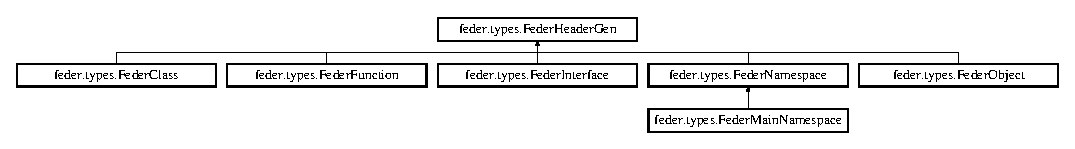
\includegraphics[height=1.555556cm]{interfacefeder_1_1types_1_1FederHeaderGen}
\end{center}
\end{figure}
\subsection*{Public Member Functions}
\begin{DoxyCompactItemize}
\item 
\mbox{\Hypertarget{interfacefeder_1_1types_1_1FederHeaderGen_aed2748617e38cb2a10549d77216e39f7}\label{interfacefeder_1_1types_1_1FederHeaderGen_aed2748617e38cb2a10549d77216e39f7}} 
String {\bfseries generate\+In\+Header} ()
\end{DoxyCompactItemize}


The documentation for this interface was generated from the following file\+:\begin{DoxyCompactItemize}
\item 
src/feder/types/Feder\+Header\+Gen.\+java\end{DoxyCompactItemize}

\hypertarget{classfeder_1_1types_1_1FederInterface}{}\section{feder.\+types.\+Feder\+Interface Class Reference}
\label{classfeder_1_1types_1_1FederInterface}\index{feder.\+types.\+Feder\+Interface@{feder.\+types.\+Feder\+Interface}}
Inheritance diagram for feder.\+types.\+Feder\+Interface\+:\begin{figure}[H]
\begin{center}
\leavevmode
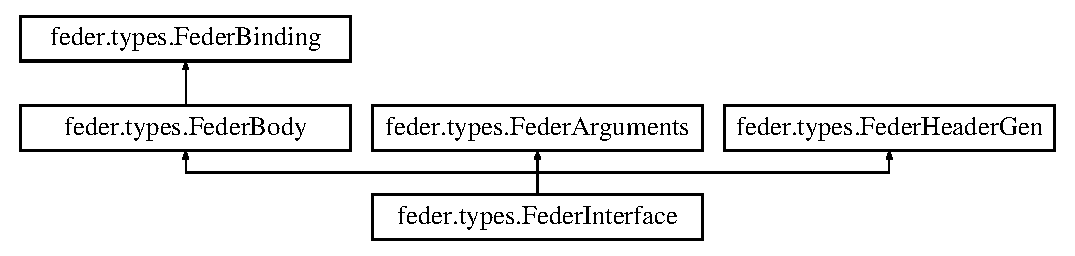
\includegraphics[height=2.994653cm]{classfeder_1_1types_1_1FederInterface}
\end{center}
\end{figure}
\subsection*{Public Member Functions}
\begin{DoxyCompactItemize}
\item 
\hyperlink{classfeder_1_1types_1_1FederInterface_abf8041a965038ca41879cecb74978b23}{Feder\+Interface} (\hyperlink{classfeder_1_1FederCompiler}{Feder\+Compiler} compiler0, String name0, \hyperlink{classfeder_1_1types_1_1FederBody}{Feder\+Body} parent)
\item 
\mbox{\Hypertarget{classfeder_1_1types_1_1FederInterface_a934a3b6f546097139d839012754f8d39}\label{classfeder_1_1types_1_1FederInterface_a934a3b6f546097139d839012754f8d39}} 
\hyperlink{classfeder_1_1types_1_1FederInterface}{Feder\+Interface} {\bfseries interface\+From} (\hyperlink{classfeder_1_1FederCompiler}{Feder\+Compiler} compiler0, String name, \hyperlink{classfeder_1_1types_1_1FederBody}{Feder\+Body} parent)
\item 
\mbox{\Hypertarget{classfeder_1_1types_1_1FederInterface_a38f609c2c8732592f95faf260be7edd9}\label{classfeder_1_1types_1_1FederInterface_a38f609c2c8732592f95faf260be7edd9}} 
{\bfseries Feder\+Interface} (\hyperlink{classfeder_1_1FederCompiler}{Feder\+Compiler} compiler0, String name0, \hyperlink{classfeder_1_1types_1_1FederBody}{Feder\+Body} parent, List$<$ \hyperlink{classfeder_1_1types_1_1FederObject}{Feder\+Object} $>$ arguments0, \hyperlink{classfeder_1_1types_1_1FederBinding}{Feder\+Binding} return\+Type0)
\item 
\mbox{\Hypertarget{classfeder_1_1types_1_1FederInterface_aeb4995b722e176b73a9a128d7047de9b}\label{classfeder_1_1types_1_1FederInterface_aeb4995b722e176b73a9a128d7047de9b}} 
String {\bfseries generate\+C\+Name} ()
\item 
\mbox{\Hypertarget{classfeder_1_1types_1_1FederInterface_aa84c636d337ec5e39f5b3bf51587b4ae}\label{classfeder_1_1types_1_1FederInterface_aa84c636d337ec5e39f5b3bf51587b4ae}} 
List$<$ \hyperlink{classfeder_1_1types_1_1FederObject}{Feder\+Object} $>$ {\bfseries get\+Arguments} ()
\item 
\mbox{\Hypertarget{classfeder_1_1types_1_1FederInterface_ae707b0cfcde306b04c757d554178e6ee}\label{classfeder_1_1types_1_1FederInterface_ae707b0cfcde306b04c757d554178e6ee}} 
boolean {\bfseries is\+Equal} (String name, List$<$ \hyperlink{classfeder_1_1types_1_1FederBinding}{Feder\+Binding} $>$ arguments0)
\item 
\hyperlink{classfeder_1_1types_1_1FederBinding}{Feder\+Binding} \hyperlink{classfeder_1_1types_1_1FederInterface_a3fecf39c73125eeaf51a33ddfbdc9f91}{get\+Return\+Type} ()
\item 
\mbox{\Hypertarget{classfeder_1_1types_1_1FederInterface_a726d0bf8d4fcfac49ca08b8f18a89e33}\label{classfeder_1_1types_1_1FederInterface_a726d0bf8d4fcfac49ca08b8f18a89e33}} 
void {\bfseries set\+Return\+Type} (\hyperlink{classfeder_1_1types_1_1FederBinding}{Feder\+Binding} fc)
\item 
\mbox{\Hypertarget{classfeder_1_1types_1_1FederInterface_a42f08a4aecfb2c64278f8ae95c01e29d}\label{classfeder_1_1types_1_1FederInterface_a42f08a4aecfb2c64278f8ae95c01e29d}} 
boolean {\bfseries can\+Be\+Called} ()
\item 
\mbox{\Hypertarget{classfeder_1_1types_1_1FederInterface_aab048e723c0f711346828ba7ceca074b}\label{classfeder_1_1types_1_1FederInterface_aab048e723c0f711346828ba7ceca074b}} 
String {\bfseries generate\+In\+Header} ()
\item 
\mbox{\Hypertarget{classfeder_1_1types_1_1FederInterface_a821190cccc9161fa3059306794212616}\label{classfeder_1_1types_1_1FederInterface_a821190cccc9161fa3059306794212616}} 
boolean {\bfseries similiar\+To\+Arguments} (\hyperlink{interfacefeder_1_1types_1_1FederArguments}{Feder\+Arguments} args)
\end{DoxyCompactItemize}
\subsection*{Public Attributes}
\begin{DoxyCompactItemize}
\item 
\mbox{\Hypertarget{classfeder_1_1types_1_1FederInterface_a78442c5baa0cb3b5c86deece8ddd5654}\label{classfeder_1_1types_1_1FederInterface_a78442c5baa0cb3b5c86deece8ddd5654}} 
List$<$ \hyperlink{classfeder_1_1types_1_1FederObject}{Feder\+Object} $>$ {\bfseries arguments} = new Linked\+List$<$$>$()
\item 
\mbox{\Hypertarget{classfeder_1_1types_1_1FederInterface_a9bb2f944bfe9f72fda9716168203cca8}\label{classfeder_1_1types_1_1FederInterface_a9bb2f944bfe9f72fda9716168203cca8}} 
\hyperlink{classfeder_1_1types_1_1FederBinding}{Feder\+Binding} {\bfseries return\+Type}
\end{DoxyCompactItemize}
\subsection*{Additional Inherited Members}


\subsection{Detailed Description}
\begin{DoxyAuthor}{Author}
Fionn Langhans 
\end{DoxyAuthor}


\subsection{Constructor \& Destructor Documentation}
\mbox{\Hypertarget{classfeder_1_1types_1_1FederInterface_abf8041a965038ca41879cecb74978b23}\label{classfeder_1_1types_1_1FederInterface_abf8041a965038ca41879cecb74978b23}} 
\index{feder\+::types\+::\+Feder\+Interface@{feder\+::types\+::\+Feder\+Interface}!Feder\+Interface@{Feder\+Interface}}
\index{Feder\+Interface@{Feder\+Interface}!feder\+::types\+::\+Feder\+Interface@{feder\+::types\+::\+Feder\+Interface}}
\subsubsection{\texorpdfstring{Feder\+Interface()}{FederInterface()}}
{\footnotesize\ttfamily feder.\+types.\+Feder\+Interface.\+Feder\+Interface (\begin{DoxyParamCaption}\item[{\hyperlink{classfeder_1_1FederCompiler}{Feder\+Compiler}}]{compiler0,  }\item[{String}]{name0,  }\item[{\hyperlink{classfeder_1_1types_1_1FederBody}{Feder\+Body}}]{parent }\end{DoxyParamCaption})}


\begin{DoxyParams}{Parameters}
{\em name0} & Name of the Interface \\
\hline
\end{DoxyParams}


\subsection{Member Function Documentation}
\mbox{\Hypertarget{classfeder_1_1types_1_1FederInterface_a3fecf39c73125eeaf51a33ddfbdc9f91}\label{classfeder_1_1types_1_1FederInterface_a3fecf39c73125eeaf51a33ddfbdc9f91}} 
\index{feder\+::types\+::\+Feder\+Interface@{feder\+::types\+::\+Feder\+Interface}!get\+Return\+Type@{get\+Return\+Type}}
\index{get\+Return\+Type@{get\+Return\+Type}!feder\+::types\+::\+Feder\+Interface@{feder\+::types\+::\+Feder\+Interface}}
\subsubsection{\texorpdfstring{get\+Return\+Type()}{getReturnType()}}
{\footnotesize\ttfamily \hyperlink{classfeder_1_1types_1_1FederBinding}{Feder\+Binding} feder.\+types.\+Feder\+Interface.\+get\+Return\+Type (\begin{DoxyParamCaption}{ }\end{DoxyParamCaption})}

\begin{DoxyReturn}{Returns}
Can be null, otherwise this returns what class the function returns 
\end{DoxyReturn}


Implements \hyperlink{interfacefeder_1_1types_1_1FederArguments}{feder.\+types.\+Feder\+Arguments}.



The documentation for this class was generated from the following file\+:\begin{DoxyCompactItemize}
\item 
src/feder/types/Feder\+Interface.\+java\end{DoxyCompactItemize}

\hypertarget{classfeder_1_1types_1_1FederMainNamespace}{}\section{feder.\+types.\+Feder\+Main\+Namespace Class Reference}
\label{classfeder_1_1types_1_1FederMainNamespace}\index{feder.\+types.\+Feder\+Main\+Namespace@{feder.\+types.\+Feder\+Main\+Namespace}}
Inheritance diagram for feder.\+types.\+Feder\+Main\+Namespace\+:\begin{figure}[H]
\begin{center}
\leavevmode
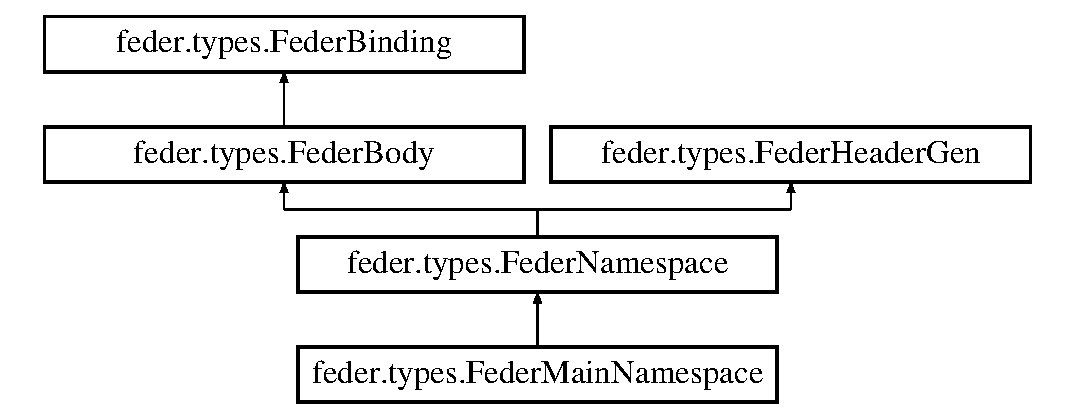
\includegraphics[height=4.000000cm]{classfeder_1_1types_1_1FederMainNamespace}
\end{center}
\end{figure}
\subsection*{Public Member Functions}
\begin{DoxyCompactItemize}
\item 
\mbox{\Hypertarget{classfeder_1_1types_1_1FederMainNamespace_a827a539f2a14818a243a13e99260ed2c}\label{classfeder_1_1types_1_1FederMainNamespace_a827a539f2a14818a243a13e99260ed2c}} 
{\bfseries Feder\+Main\+Namespace} (\hyperlink{classfeder_1_1FederCompiler}{Feder\+Compiler} compiler0, String name0, \hyperlink{classfeder_1_1types_1_1FederBody}{Feder\+Body} parent0)
\end{DoxyCompactItemize}
\subsection*{Additional Inherited Members}


The documentation for this class was generated from the following file\+:\begin{DoxyCompactItemize}
\item 
src/feder/types/Feder\+Main\+Namespace.\+java\end{DoxyCompactItemize}

\hypertarget{classfeder_1_1types_1_1FederNamespace}{}\section{feder.\+types.\+Feder\+Namespace Class Reference}
\label{classfeder_1_1types_1_1FederNamespace}\index{feder.\+types.\+Feder\+Namespace@{feder.\+types.\+Feder\+Namespace}}
Inheritance diagram for feder.\+types.\+Feder\+Namespace\+:\begin{figure}[H]
\begin{center}
\leavevmode
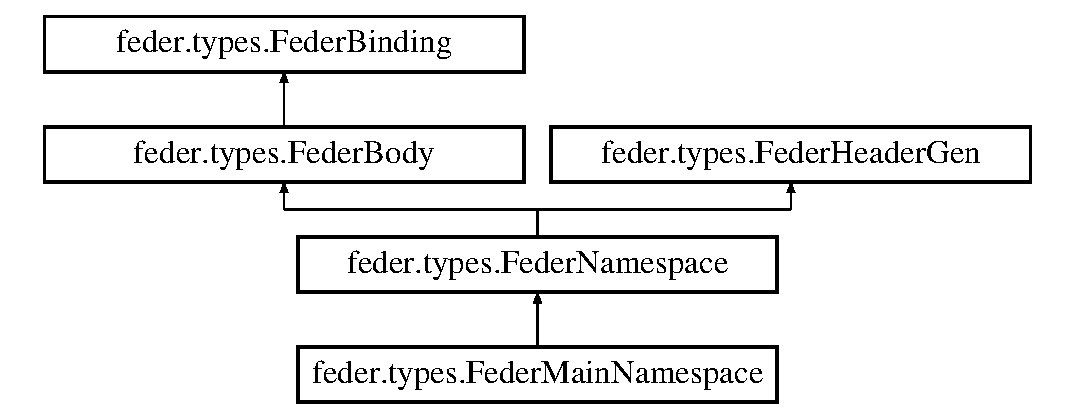
\includegraphics[height=4.000000cm]{classfeder_1_1types_1_1FederNamespace}
\end{center}
\end{figure}
\subsection*{Public Member Functions}
\begin{DoxyCompactItemize}
\item 
\mbox{\Hypertarget{classfeder_1_1types_1_1FederNamespace_a8e56d5fadf40b301143cf9303b945608}\label{classfeder_1_1types_1_1FederNamespace_a8e56d5fadf40b301143cf9303b945608}} 
{\bfseries Feder\+Namespace} (\hyperlink{classfeder_1_1FederCompiler}{Feder\+Compiler} compiler0, String name0, \hyperlink{classfeder_1_1types_1_1FederBody}{Feder\+Body} parent0)
\item 
\mbox{\Hypertarget{classfeder_1_1types_1_1FederNamespace_ac8c1560fe99728182db8bfc334827a25}\label{classfeder_1_1types_1_1FederNamespace_ac8c1560fe99728182db8bfc334827a25}} 
String {\bfseries generate\+C\+Name} ()
\item 
\mbox{\Hypertarget{classfeder_1_1types_1_1FederNamespace_a1ba6fd322c097dd392c26df468d27aea}\label{classfeder_1_1types_1_1FederNamespace_a1ba6fd322c097dd392c26df468d27aea}} 
String {\bfseries generate\+In\+Header} ()
\end{DoxyCompactItemize}
\subsection*{Additional Inherited Members}


The documentation for this class was generated from the following file\+:\begin{DoxyCompactItemize}
\item 
src/feder/types/Feder\+Namespace.\+java\end{DoxyCompactItemize}

\hypertarget{classfeder_1_1types_1_1FederObject}{}\section{feder.\+types.\+Feder\+Object Class Reference}
\label{classfeder_1_1types_1_1FederObject}\index{feder.\+types.\+Feder\+Object@{feder.\+types.\+Feder\+Object}}
Inheritance diagram for feder.\+types.\+Feder\+Object\+:\begin{figure}[H]
\begin{center}
\leavevmode
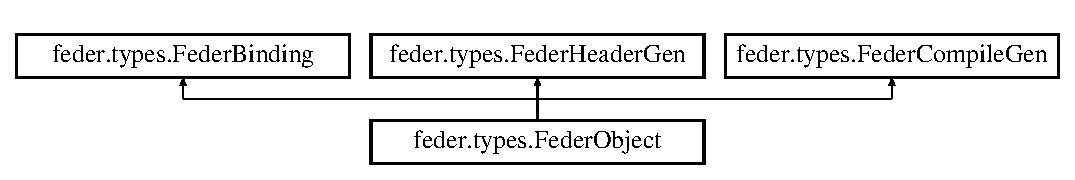
\includegraphics[height=1.964912cm]{classfeder_1_1types_1_1FederObject}
\end{center}
\end{figure}
\subsection*{Public Member Functions}
\begin{DoxyCompactItemize}
\item 
\hyperlink{classfeder_1_1types_1_1FederObject_aeb1732353aa6704a36fcf17ed22fb4a5}{Feder\+Object} (String name0, \hyperlink{classfeder_1_1types_1_1FederBody}{Feder\+Body} parent0)
\item 
\mbox{\Hypertarget{classfeder_1_1types_1_1FederObject_a5ecb7f0d59ee850fa72a587453df2c5b}\label{classfeder_1_1types_1_1FederObject_a5ecb7f0d59ee850fa72a587453df2c5b}} 
boolean {\bfseries has\+To\+Build} ()
\item 
\mbox{\Hypertarget{classfeder_1_1types_1_1FederObject_af845d4ec611829f585906a0fc5e59f64}\label{classfeder_1_1types_1_1FederObject_af845d4ec611829f585906a0fc5e59f64}} 
void {\bfseries set\+Has\+To\+Build} (boolean b)
\item 
\mbox{\Hypertarget{classfeder_1_1types_1_1FederObject_ad0e1f8753b4b03d0696e62034e134d46}\label{classfeder_1_1types_1_1FederObject_ad0e1f8753b4b03d0696e62034e134d46}} 
\hyperlink{classfeder_1_1types_1_1FederBody}{Feder\+Body} {\bfseries get\+Parent} ()
\item 
\mbox{\Hypertarget{classfeder_1_1types_1_1FederObject_a79fb75fa1f32698afcd869b6b1d3e80f}\label{classfeder_1_1types_1_1FederObject_a79fb75fa1f32698afcd869b6b1d3e80f}} 
boolean {\bfseries is\+Type} (\hyperlink{classfeder_1_1types_1_1FederBinding}{Feder\+Binding} binding)
\item 
boolean \hyperlink{classfeder_1_1types_1_1FederObject_a02dd0040b45efef9ebc21015c04f9f68}{is\+Interface} ()
\item 
boolean \hyperlink{classfeder_1_1types_1_1FederObject_af28926b03ecb38e8d622db9d8857430c}{is\+Data\+Type} ()
\item 
boolean \hyperlink{classfeder_1_1types_1_1FederObject_ab7dfff2509df360900b2680fa1ef06fb}{is\+Array} ()
\item 
\mbox{\Hypertarget{classfeder_1_1types_1_1FederObject_a0f027f65d3acb0b2ac8ba619197002f4}\label{classfeder_1_1types_1_1FederObject_a0f027f65d3acb0b2ac8ba619197002f4}} 
boolean {\bfseries is\+Class\+Object} ()
\item 
\mbox{\Hypertarget{classfeder_1_1types_1_1FederObject_a4e16ffb73532cdc8b7777ca3169fa3d6}\label{classfeder_1_1types_1_1FederObject_a4e16ffb73532cdc8b7777ca3169fa3d6}} 
boolean {\bfseries has\+Subtypes} ()
\item 
void \hyperlink{classfeder_1_1types_1_1FederObject_a45257f7c53f6959f12bf85b32137772b}{set\+Type\+Intelligent} (\hyperlink{classfeder_1_1types_1_1FederBinding}{Feder\+Binding} bind)
\item 
void \hyperlink{classfeder_1_1types_1_1FederObject_a474b468bf57e328bcc31b10a2e2cb346}{set\+Type\+Manual} (\hyperlink{classfeder_1_1types_1_1FederBinding}{Feder\+Binding} bind)
\item 
\hyperlink{classfeder_1_1types_1_1FederBinding}{Feder\+Binding} \hyperlink{classfeder_1_1types_1_1FederObject_a6eb6a31ce2468538288aac6aa0cca06a}{get\+Result\+Type} ()
\item 
boolean \hyperlink{classfeder_1_1types_1_1FederObject_a2d4a3bbd8a43871e08b9fe418a3ce2ad}{is\+Garbagable} ()
\item 
String \hyperlink{classfeder_1_1types_1_1FederObject_afced6ab112045e9757c40bd06ac6413c}{get\+Name} ()
\item 
String \hyperlink{classfeder_1_1types_1_1FederObject_a455578a3f7a79b56512c7a6eeebe676c}{generate\+C\+Name} ()
\item 
String \hyperlink{classfeder_1_1types_1_1FederObject_ada1a393c691be4b1cded1a59936d58af}{generate\+C\+Name\+Only} ()
\item 
String \hyperlink{classfeder_1_1types_1_1FederObject_a4e813a7bd196036c8754ef35bcffbfef}{generate\+In\+Header} ()
\item 
String \hyperlink{classfeder_1_1types_1_1FederObject_abd2747e5a73af451a3280fecb1afa12b}{generate\+In\+Compile} ()
\item 
String \hyperlink{classfeder_1_1types_1_1FederObject_ab606323254677bef8b0b1afe1377e073}{get\+Code\+Friendly\+Name} ()
\end{DoxyCompactItemize}
\subsection*{Public Attributes}
\begin{DoxyCompactItemize}
\item 
boolean \hyperlink{classfeder_1_1types_1_1FederObject_ae0f93d5fc5f91116c42ec7818470d87b}{is\+Forced} = false
\item 
\hyperlink{classfeder_1_1types_1_1FederBody}{Feder\+Body} \hyperlink{classfeder_1_1types_1_1FederObject_a20004c8220590134967231ab27d55b03}{parent} = null
\item 
boolean \hyperlink{classfeder_1_1types_1_1FederObject_a1779800250bc3af84e2c49def2cad2d4}{is\+Global} = false
\item 
boolean \hyperlink{classfeder_1_1types_1_1FederObject_a195c2873c269f7719e727ddf7af62996}{is\+Out} = false
\item 
boolean \hyperlink{classfeder_1_1types_1_1FederObject_a506fd435faadb7ca7e9a79e64d998acd}{raw\+\_\+c\+\_\+gen} = false
\end{DoxyCompactItemize}
\subsection*{Additional Inherited Members}


\subsection{Detailed Description}
Representing a object in \hyperlink{classfeder_1_1Feder}{Feder} \begin{DoxyAuthor}{Author}
Fionn Langhans 
\end{DoxyAuthor}


\subsection{Constructor \& Destructor Documentation}
\mbox{\Hypertarget{classfeder_1_1types_1_1FederObject_aeb1732353aa6704a36fcf17ed22fb4a5}\label{classfeder_1_1types_1_1FederObject_aeb1732353aa6704a36fcf17ed22fb4a5}} 
\index{feder\+::types\+::\+Feder\+Object@{feder\+::types\+::\+Feder\+Object}!Feder\+Object@{Feder\+Object}}
\index{Feder\+Object@{Feder\+Object}!feder\+::types\+::\+Feder\+Object@{feder\+::types\+::\+Feder\+Object}}
\subsubsection{\texorpdfstring{Feder\+Object()}{FederObject()}}
{\footnotesize\ttfamily feder.\+types.\+Feder\+Object.\+Feder\+Object (\begin{DoxyParamCaption}\item[{String}]{name0,  }\item[{\hyperlink{classfeder_1_1types_1_1FederBody}{Feder\+Body}}]{parent0 }\end{DoxyParamCaption})}


\begin{DoxyParams}{Parameters}
{\em name0} & the name of binding \\
\hline
{\em parent0} & the parent of this object (can be null, but sometimes not) \\
\hline
\end{DoxyParams}


\subsection{Member Function Documentation}
\mbox{\Hypertarget{classfeder_1_1types_1_1FederObject_a455578a3f7a79b56512c7a6eeebe676c}\label{classfeder_1_1types_1_1FederObject_a455578a3f7a79b56512c7a6eeebe676c}} 
\index{feder\+::types\+::\+Feder\+Object@{feder\+::types\+::\+Feder\+Object}!generate\+C\+Name@{generate\+C\+Name}}
\index{generate\+C\+Name@{generate\+C\+Name}!feder\+::types\+::\+Feder\+Object@{feder\+::types\+::\+Feder\+Object}}
\subsubsection{\texorpdfstring{generate\+C\+Name()}{generateCName()}}
{\footnotesize\ttfamily String feder.\+types.\+Feder\+Object.\+generate\+C\+Name (\begin{DoxyParamCaption}{ }\end{DoxyParamCaption})}

\begin{DoxyReturn}{Returns}
the name to use in C source code 
\end{DoxyReturn}
\mbox{\Hypertarget{classfeder_1_1types_1_1FederObject_ada1a393c691be4b1cded1a59936d58af}\label{classfeder_1_1types_1_1FederObject_ada1a393c691be4b1cded1a59936d58af}} 
\index{feder\+::types\+::\+Feder\+Object@{feder\+::types\+::\+Feder\+Object}!generate\+C\+Name\+Only@{generate\+C\+Name\+Only}}
\index{generate\+C\+Name\+Only@{generate\+C\+Name\+Only}!feder\+::types\+::\+Feder\+Object@{feder\+::types\+::\+Feder\+Object}}
\subsubsection{\texorpdfstring{generate\+C\+Name\+Only()}{generateCNameOnly()}}
{\footnotesize\ttfamily String feder.\+types.\+Feder\+Object.\+generate\+C\+Name\+Only (\begin{DoxyParamCaption}{ }\end{DoxyParamCaption})}

\begin{DoxyReturn}{Returns}
Returns the C source code name without any memory modifiers 
\end{DoxyReturn}
\mbox{\Hypertarget{classfeder_1_1types_1_1FederObject_abd2747e5a73af451a3280fecb1afa12b}\label{classfeder_1_1types_1_1FederObject_abd2747e5a73af451a3280fecb1afa12b}} 
\index{feder\+::types\+::\+Feder\+Object@{feder\+::types\+::\+Feder\+Object}!generate\+In\+Compile@{generate\+In\+Compile}}
\index{generate\+In\+Compile@{generate\+In\+Compile}!feder\+::types\+::\+Feder\+Object@{feder\+::types\+::\+Feder\+Object}}
\subsubsection{\texorpdfstring{generate\+In\+Compile()}{generateInCompile()}}
{\footnotesize\ttfamily String feder.\+types.\+Feder\+Object.\+generate\+In\+Compile (\begin{DoxyParamCaption}{ }\end{DoxyParamCaption})}

\begin{DoxyReturn}{Returns}
Returns a string, which should be generated in the compile/code file 
\end{DoxyReturn}


Implements \hyperlink{interfacefeder_1_1types_1_1FederCompileGen}{feder.\+types.\+Feder\+Compile\+Gen}.

\mbox{\Hypertarget{classfeder_1_1types_1_1FederObject_a4e813a7bd196036c8754ef35bcffbfef}\label{classfeder_1_1types_1_1FederObject_a4e813a7bd196036c8754ef35bcffbfef}} 
\index{feder\+::types\+::\+Feder\+Object@{feder\+::types\+::\+Feder\+Object}!generate\+In\+Header@{generate\+In\+Header}}
\index{generate\+In\+Header@{generate\+In\+Header}!feder\+::types\+::\+Feder\+Object@{feder\+::types\+::\+Feder\+Object}}
\subsubsection{\texorpdfstring{generate\+In\+Header()}{generateInHeader()}}
{\footnotesize\ttfamily String feder.\+types.\+Feder\+Object.\+generate\+In\+Header (\begin{DoxyParamCaption}{ }\end{DoxyParamCaption})}

\begin{DoxyReturn}{Returns}
Returns a string, which should be generated in the header file 
\end{DoxyReturn}


Implements \hyperlink{interfacefeder_1_1types_1_1FederHeaderGen}{feder.\+types.\+Feder\+Header\+Gen}.

\mbox{\Hypertarget{classfeder_1_1types_1_1FederObject_ab606323254677bef8b0b1afe1377e073}\label{classfeder_1_1types_1_1FederObject_ab606323254677bef8b0b1afe1377e073}} 
\index{feder\+::types\+::\+Feder\+Object@{feder\+::types\+::\+Feder\+Object}!get\+Code\+Friendly\+Name@{get\+Code\+Friendly\+Name}}
\index{get\+Code\+Friendly\+Name@{get\+Code\+Friendly\+Name}!feder\+::types\+::\+Feder\+Object@{feder\+::types\+::\+Feder\+Object}}
\subsubsection{\texorpdfstring{get\+Code\+Friendly\+Name()}{getCodeFriendlyName()}}
{\footnotesize\ttfamily String feder.\+types.\+Feder\+Object.\+get\+Code\+Friendly\+Name (\begin{DoxyParamCaption}{ }\end{DoxyParamCaption})}

\begin{DoxyReturn}{Returns}
the object\textquotesingle{}s name is a code friendly name, so \hyperlink{classfeder_1_1types_1_1FederObject_afced6ab112045e9757c40bd06ac6413c}{get\+Name } is returned. 
\end{DoxyReturn}
\mbox{\Hypertarget{classfeder_1_1types_1_1FederObject_afced6ab112045e9757c40bd06ac6413c}\label{classfeder_1_1types_1_1FederObject_afced6ab112045e9757c40bd06ac6413c}} 
\index{feder\+::types\+::\+Feder\+Object@{feder\+::types\+::\+Feder\+Object}!get\+Name@{get\+Name}}
\index{get\+Name@{get\+Name}!feder\+::types\+::\+Feder\+Object@{feder\+::types\+::\+Feder\+Object}}
\subsubsection{\texorpdfstring{get\+Name()}{getName()}}
{\footnotesize\ttfamily String feder.\+types.\+Feder\+Object.\+get\+Name (\begin{DoxyParamCaption}{ }\end{DoxyParamCaption})}

\begin{DoxyReturn}{Returns}
T\+HE binding 
\end{DoxyReturn}
\mbox{\Hypertarget{classfeder_1_1types_1_1FederObject_a6eb6a31ce2468538288aac6aa0cca06a}\label{classfeder_1_1types_1_1FederObject_a6eb6a31ce2468538288aac6aa0cca06a}} 
\index{feder\+::types\+::\+Feder\+Object@{feder\+::types\+::\+Feder\+Object}!get\+Result\+Type@{get\+Result\+Type}}
\index{get\+Result\+Type@{get\+Result\+Type}!feder\+::types\+::\+Feder\+Object@{feder\+::types\+::\+Feder\+Object}}
\subsubsection{\texorpdfstring{get\+Result\+Type()}{getResultType()}}
{\footnotesize\ttfamily \hyperlink{classfeder_1_1types_1_1FederBinding}{Feder\+Binding} feder.\+types.\+Feder\+Object.\+get\+Result\+Type (\begin{DoxyParamCaption}{ }\end{DoxyParamCaption})}

\begin{DoxyReturn}{Returns}
Returns the type of this object 
\end{DoxyReturn}
\mbox{\Hypertarget{classfeder_1_1types_1_1FederObject_ab7dfff2509df360900b2680fa1ef06fb}\label{classfeder_1_1types_1_1FederObject_ab7dfff2509df360900b2680fa1ef06fb}} 
\index{feder\+::types\+::\+Feder\+Object@{feder\+::types\+::\+Feder\+Object}!is\+Array@{is\+Array}}
\index{is\+Array@{is\+Array}!feder\+::types\+::\+Feder\+Object@{feder\+::types\+::\+Feder\+Object}}
\subsubsection{\texorpdfstring{is\+Array()}{isArray()}}
{\footnotesize\ttfamily boolean feder.\+types.\+Feder\+Object.\+is\+Array (\begin{DoxyParamCaption}{ }\end{DoxyParamCaption})}

\begin{DoxyReturn}{Returns}
Returns true, if the type of this object is an array. 
\end{DoxyReturn}
\mbox{\Hypertarget{classfeder_1_1types_1_1FederObject_af28926b03ecb38e8d622db9d8857430c}\label{classfeder_1_1types_1_1FederObject_af28926b03ecb38e8d622db9d8857430c}} 
\index{feder\+::types\+::\+Feder\+Object@{feder\+::types\+::\+Feder\+Object}!is\+Data\+Type@{is\+Data\+Type}}
\index{is\+Data\+Type@{is\+Data\+Type}!feder\+::types\+::\+Feder\+Object@{feder\+::types\+::\+Feder\+Object}}
\subsubsection{\texorpdfstring{is\+Data\+Type()}{isDataType()}}
{\footnotesize\ttfamily boolean feder.\+types.\+Feder\+Object.\+is\+Data\+Type (\begin{DoxyParamCaption}{ }\end{DoxyParamCaption})}

\begin{DoxyReturn}{Returns}
Returns true, if the type of this object is an datatype. 
\end{DoxyReturn}
\mbox{\Hypertarget{classfeder_1_1types_1_1FederObject_a2d4a3bbd8a43871e08b9fe418a3ce2ad}\label{classfeder_1_1types_1_1FederObject_a2d4a3bbd8a43871e08b9fe418a3ce2ad}} 
\index{feder\+::types\+::\+Feder\+Object@{feder\+::types\+::\+Feder\+Object}!is\+Garbagable@{is\+Garbagable}}
\index{is\+Garbagable@{is\+Garbagable}!feder\+::types\+::\+Feder\+Object@{feder\+::types\+::\+Feder\+Object}}
\subsubsection{\texorpdfstring{is\+Garbagable()}{isGarbagable()}}
{\footnotesize\ttfamily boolean feder.\+types.\+Feder\+Object.\+is\+Garbagable (\begin{DoxyParamCaption}{ }\end{DoxyParamCaption})}

\begin{DoxyReturn}{Returns}
Returns true, if this object can be collected by the garbage collection 
\end{DoxyReturn}
\mbox{\Hypertarget{classfeder_1_1types_1_1FederObject_a02dd0040b45efef9ebc21015c04f9f68}\label{classfeder_1_1types_1_1FederObject_a02dd0040b45efef9ebc21015c04f9f68}} 
\index{feder\+::types\+::\+Feder\+Object@{feder\+::types\+::\+Feder\+Object}!is\+Interface@{is\+Interface}}
\index{is\+Interface@{is\+Interface}!feder\+::types\+::\+Feder\+Object@{feder\+::types\+::\+Feder\+Object}}
\subsubsection{\texorpdfstring{is\+Interface()}{isInterface()}}
{\footnotesize\ttfamily boolean feder.\+types.\+Feder\+Object.\+is\+Interface (\begin{DoxyParamCaption}{ }\end{DoxyParamCaption})}

\begin{DoxyReturn}{Returns}
Returns true, if the type of this object is an interface. 
\end{DoxyReturn}
\mbox{\Hypertarget{classfeder_1_1types_1_1FederObject_a45257f7c53f6959f12bf85b32137772b}\label{classfeder_1_1types_1_1FederObject_a45257f7c53f6959f12bf85b32137772b}} 
\index{feder\+::types\+::\+Feder\+Object@{feder\+::types\+::\+Feder\+Object}!set\+Type\+Intelligent@{set\+Type\+Intelligent}}
\index{set\+Type\+Intelligent@{set\+Type\+Intelligent}!feder\+::types\+::\+Feder\+Object@{feder\+::types\+::\+Feder\+Object}}
\subsubsection{\texorpdfstring{set\+Type\+Intelligent()}{setTypeIntelligent()}}
{\footnotesize\ttfamily void feder.\+types.\+Feder\+Object.\+set\+Type\+Intelligent (\begin{DoxyParamCaption}\item[{\hyperlink{classfeder_1_1types_1_1FederBinding}{Feder\+Binding}}]{bind }\end{DoxyParamCaption})}

Checks if allowd to change type \mbox{\Hypertarget{classfeder_1_1types_1_1FederObject_a474b468bf57e328bcc31b10a2e2cb346}\label{classfeder_1_1types_1_1FederObject_a474b468bf57e328bcc31b10a2e2cb346}} 
\index{feder\+::types\+::\+Feder\+Object@{feder\+::types\+::\+Feder\+Object}!set\+Type\+Manual@{set\+Type\+Manual}}
\index{set\+Type\+Manual@{set\+Type\+Manual}!feder\+::types\+::\+Feder\+Object@{feder\+::types\+::\+Feder\+Object}}
\subsubsection{\texorpdfstring{set\+Type\+Manual()}{setTypeManual()}}
{\footnotesize\ttfamily void feder.\+types.\+Feder\+Object.\+set\+Type\+Manual (\begin{DoxyParamCaption}\item[{\hyperlink{classfeder_1_1types_1_1FederBinding}{Feder\+Binding}}]{bind }\end{DoxyParamCaption})}

Doesn\textquotesingle{}t do any checks 
\begin{DoxyParams}{Parameters}
{\em bind} & \\
\hline
\end{DoxyParams}


\subsection{Member Data Documentation}
\mbox{\Hypertarget{classfeder_1_1types_1_1FederObject_ae0f93d5fc5f91116c42ec7818470d87b}\label{classfeder_1_1types_1_1FederObject_ae0f93d5fc5f91116c42ec7818470d87b}} 
\index{feder\+::types\+::\+Feder\+Object@{feder\+::types\+::\+Feder\+Object}!is\+Forced@{is\+Forced}}
\index{is\+Forced@{is\+Forced}!feder\+::types\+::\+Feder\+Object@{feder\+::types\+::\+Feder\+Object}}
\subsubsection{\texorpdfstring{is\+Forced}{isForced}}
{\footnotesize\ttfamily boolean feder.\+types.\+Feder\+Object.\+is\+Forced = false}

Force the type of the object \mbox{\Hypertarget{classfeder_1_1types_1_1FederObject_a1779800250bc3af84e2c49def2cad2d4}\label{classfeder_1_1types_1_1FederObject_a1779800250bc3af84e2c49def2cad2d4}} 
\index{feder\+::types\+::\+Feder\+Object@{feder\+::types\+::\+Feder\+Object}!is\+Global@{is\+Global}}
\index{is\+Global@{is\+Global}!feder\+::types\+::\+Feder\+Object@{feder\+::types\+::\+Feder\+Object}}
\subsubsection{\texorpdfstring{is\+Global}{isGlobal}}
{\footnotesize\ttfamily boolean feder.\+types.\+Feder\+Object.\+is\+Global = false}

Is the object global ? \mbox{\Hypertarget{classfeder_1_1types_1_1FederObject_a195c2873c269f7719e727ddf7af62996}\label{classfeder_1_1types_1_1FederObject_a195c2873c269f7719e727ddf7af62996}} 
\index{feder\+::types\+::\+Feder\+Object@{feder\+::types\+::\+Feder\+Object}!is\+Out@{is\+Out}}
\index{is\+Out@{is\+Out}!feder\+::types\+::\+Feder\+Object@{feder\+::types\+::\+Feder\+Object}}
\subsubsection{\texorpdfstring{is\+Out}{isOut}}
{\footnotesize\ttfamily boolean feder.\+types.\+Feder\+Object.\+is\+Out = false}

Is the object an \textquotesingle{}out\textquotesingle{} object (an extra pointer is necessary) ? \mbox{\Hypertarget{classfeder_1_1types_1_1FederObject_a20004c8220590134967231ab27d55b03}\label{classfeder_1_1types_1_1FederObject_a20004c8220590134967231ab27d55b03}} 
\index{feder\+::types\+::\+Feder\+Object@{feder\+::types\+::\+Feder\+Object}!parent@{parent}}
\index{parent@{parent}!feder\+::types\+::\+Feder\+Object@{feder\+::types\+::\+Feder\+Object}}
\subsubsection{\texorpdfstring{parent}{parent}}
{\footnotesize\ttfamily \hyperlink{classfeder_1_1types_1_1FederBody}{Feder\+Body} feder.\+types.\+Feder\+Object.\+parent = null}

The parent of this object \mbox{\Hypertarget{classfeder_1_1types_1_1FederObject_a506fd435faadb7ca7e9a79e64d998acd}\label{classfeder_1_1types_1_1FederObject_a506fd435faadb7ca7e9a79e64d998acd}} 
\index{feder\+::types\+::\+Feder\+Object@{feder\+::types\+::\+Feder\+Object}!raw\+\_\+c\+\_\+gen@{raw\+\_\+c\+\_\+gen}}
\index{raw\+\_\+c\+\_\+gen@{raw\+\_\+c\+\_\+gen}!feder\+::types\+::\+Feder\+Object@{feder\+::types\+::\+Feder\+Object}}
\subsubsection{\texorpdfstring{raw\+\_\+c\+\_\+gen}{raw\_c\_gen}}
{\footnotesize\ttfamily boolean feder.\+types.\+Feder\+Object.\+raw\+\_\+c\+\_\+gen = false}

Use the object\textquotesingle{}s name directly as C name 

The documentation for this class was generated from the following file\+:\begin{DoxyCompactItemize}
\item 
src/feder/types/Feder\+Object.\+java\end{DoxyCompactItemize}

\hypertarget{classfeder_1_1types_1_1FederRule}{}\section{feder.\+types.\+Feder\+Rule Class Reference}
\label{classfeder_1_1types_1_1FederRule}\index{feder.\+types.\+Feder\+Rule@{feder.\+types.\+Feder\+Rule}}
\subsection*{Public Member Functions}
\begin{DoxyCompactItemize}
\item 
\mbox{\Hypertarget{classfeder_1_1types_1_1FederRule_a8ee9a0e9afcfda997e4319488e399aa2}\label{classfeder_1_1types_1_1FederRule_a8ee9a0e9afcfda997e4319488e399aa2}} 
{\bfseries Feder\+Rule} (int rule0, String operator0, String to\+Apply0, \hyperlink{classfeder_1_1types_1_1FederBinding}{Feder\+Binding} return\+Value0, \hyperlink{classfeder_1_1types_1_1FederBinding}{Feder\+Binding} lvalue0, \hyperlink{classfeder_1_1types_1_1FederBinding}{Feder\+Binding} rvalue0)
\item 
\mbox{\Hypertarget{classfeder_1_1types_1_1FederRule_a1ea7da26513e2295dc7d5ae8a7d7dcc1}\label{classfeder_1_1types_1_1FederRule_a1ea7da26513e2295dc7d5ae8a7d7dcc1}} 
{\bfseries Feder\+Rule} (int rule0, String buildin\+\_\+name, String to\+Apply0, \hyperlink{classfeder_1_1types_1_1FederBinding}{Feder\+Binding} result)
\item 
\mbox{\Hypertarget{classfeder_1_1types_1_1FederRule_a49becaf0f19cff6aeb71097e365e254a}\label{classfeder_1_1types_1_1FederRule_a49becaf0f19cff6aeb71097e365e254a}} 
{\bfseries Feder\+Rule} (int rule0, String operator0, \hyperlink{interfacefeder_1_1types_1_1FederArguments}{Feder\+Arguments} func)
\item 
\mbox{\Hypertarget{classfeder_1_1types_1_1FederRule_a1c179e28c0f5def95a910cbd138f0bfb}\label{classfeder_1_1types_1_1FederRule_a1c179e28c0f5def95a910cbd138f0bfb}} 
{\bfseries Feder\+Rule} (int rule0, String operator0, String to\+Apply0)
\item 
boolean \hyperlink{classfeder_1_1types_1_1FederRule_afcc217a0afa07a0a6eb6a3bbe3cfb70a}{is\+Applyable} (String buildin)
\item 
\mbox{\Hypertarget{classfeder_1_1types_1_1FederRule_a7677e9211a5c4e4edd62462c85a437c5}\label{classfeder_1_1types_1_1FederRule_a7677e9211a5c4e4edd62462c85a437c5}} 
String {\bfseries apply\+Rule} (\hyperlink{classfeder_1_1types_1_1FederBody}{Feder\+Body} current\+Body, String buildin)
\item 
boolean \hyperlink{classfeder_1_1types_1_1FederRule_a90ca7877e026698624a675f72783e7d2}{is\+Applyable} (String operator0, \hyperlink{classfeder_1_1types_1_1FederBinding}{Feder\+Binding} lvalue0, \hyperlink{classfeder_1_1types_1_1FederBinding}{Feder\+Binding} rvalue0)
\item 
String \hyperlink{classfeder_1_1types_1_1FederRule_a3df175f196c684adb0ef4fa99a2599e0}{apply\+Rule} (\hyperlink{classfeder_1_1types_1_1FederBody}{Feder\+Body} current\+Body, String lstring, String rstring)
\item 
\hyperlink{classfeder_1_1types_1_1FederBinding}{Feder\+Binding} \hyperlink{classfeder_1_1types_1_1FederRule_a6de23e91ac085ac4fb0de47389d554bf}{get\+L\+Value} ()
\item 
\hyperlink{classfeder_1_1types_1_1FederBinding}{Feder\+Binding} \hyperlink{classfeder_1_1types_1_1FederRule_a306bb79d403d4de804ece5ae47c0d524}{get\+R\+Value} ()
\item 
\hyperlink{classfeder_1_1types_1_1FederBinding}{Feder\+Binding} \hyperlink{classfeder_1_1types_1_1FederRule_a48e0b9aca68eff113f51c03a3198ff70}{get\+Result\+Value} ()
\item 
int \hyperlink{classfeder_1_1types_1_1FederRule_a2463391941d5dc6afefa1e672fc1c62d}{get\+Rule} ()
\item 
\mbox{\Hypertarget{classfeder_1_1types_1_1FederRule_af9083a73f755838ce38360b15fb3433a}\label{classfeder_1_1types_1_1FederRule_af9083a73f755838ce38360b15fb3433a}} 
String {\bfseries get\+Operator} ()
\item 
\mbox{\Hypertarget{classfeder_1_1types_1_1FederRule_a379510a2a05eab4ed04c37d09c6ded0e}\label{classfeder_1_1types_1_1FederRule_a379510a2a05eab4ed04c37d09c6ded0e}} 
String {\bfseries get\+To\+Apply} ()
\end{DoxyCompactItemize}
\subsection*{Static Public Member Functions}
\begin{DoxyCompactItemize}
\item 
static final \hyperlink{classfeder_1_1types_1_1FederRule}{Feder\+Rule} \hyperlink{classfeder_1_1types_1_1FederRule_af2842318a6287f4096af22d056feda29}{define} (\hyperlink{classfeder_1_1types_1_1FederBody}{Feder\+Body} current\+Body, List$<$ String $>$ args, \hyperlink{classfeder_1_1SyntaxTreeElement}{Syntax\+Tree\+Element} ste)
\end{DoxyCompactItemize}
\subsection*{Static Public Attributes}
\begin{DoxyCompactItemize}
\item 
static final int \hyperlink{classfeder_1_1types_1_1FederRule_ac52e0e9fa01933aae9043c8db8c6756e}{R\+U\+L\+E\+\_\+\+O\+P\+E\+R\+A\+T\+OR} = 0x0001
\item 
static final int \hyperlink{classfeder_1_1types_1_1FederRule_a848abbbabef84c98beb5b83fcd8c5123}{R\+U\+L\+E\+\_\+\+A\+S\+S\+I\+G\+N\+M\+E\+NT} = 0x0002
\item 
static final int \hyperlink{classfeder_1_1types_1_1FederRule_a0299f2160aaab5b54997fb1c835bb034}{R\+U\+L\+E\+\_\+\+T\+Y\+PE} = 0x0004
\item 
static final int \hyperlink{classfeder_1_1types_1_1FederRule_ab1aceaccc1e229d42eb86de6cbeb7a7d}{R\+U\+L\+E\+\_\+\+F\+U\+N\+C\+T\+I\+ON} = 0x0100
\item 
static final int \hyperlink{classfeder_1_1types_1_1FederRule_a417762d710fd8cf2964d4ae67c6b054f}{R\+U\+L\+E\+\_\+\+P\+A\+T\+T\+E\+RN} = 0x0200
\item 
static final int \hyperlink{classfeder_1_1types_1_1FederRule_a1140c3933b8ad6b86b34a829bf243f52}{R\+U\+L\+E\+\_\+\+B\+U\+I\+L\+D\+IN} = 0x0400
\item 
static final int \hyperlink{classfeder_1_1types_1_1FederRule_aaacf50868fe27de3125ca4293915e1c2}{R\+U\+L\+E\+\_\+\+S\+T\+R\+U\+CT} = 0x0800
\end{DoxyCompactItemize}


\subsection{Detailed Description}
\begin{DoxyAuthor}{Author}
Fionn Langhans 
\end{DoxyAuthor}


\subsection{Member Function Documentation}
\mbox{\Hypertarget{classfeder_1_1types_1_1FederRule_a3df175f196c684adb0ef4fa99a2599e0}\label{classfeder_1_1types_1_1FederRule_a3df175f196c684adb0ef4fa99a2599e0}} 
\index{feder\+::types\+::\+Feder\+Rule@{feder\+::types\+::\+Feder\+Rule}!apply\+Rule@{apply\+Rule}}
\index{apply\+Rule@{apply\+Rule}!feder\+::types\+::\+Feder\+Rule@{feder\+::types\+::\+Feder\+Rule}}
\subsubsection{\texorpdfstring{apply\+Rule()}{applyRule()}}
{\footnotesize\ttfamily String feder.\+types.\+Feder\+Rule.\+apply\+Rule (\begin{DoxyParamCaption}\item[{\hyperlink{classfeder_1_1types_1_1FederBody}{Feder\+Body}}]{current\+Body,  }\item[{String}]{lstring,  }\item[{String}]{rstring }\end{DoxyParamCaption})}

\begin{DoxyReturn}{Returns}
Returns the result of the rule 
\end{DoxyReturn}
\mbox{\Hypertarget{classfeder_1_1types_1_1FederRule_af2842318a6287f4096af22d056feda29}\label{classfeder_1_1types_1_1FederRule_af2842318a6287f4096af22d056feda29}} 
\index{feder\+::types\+::\+Feder\+Rule@{feder\+::types\+::\+Feder\+Rule}!define@{define}}
\index{define@{define}!feder\+::types\+::\+Feder\+Rule@{feder\+::types\+::\+Feder\+Rule}}
\subsubsection{\texorpdfstring{define()}{define()}}
{\footnotesize\ttfamily static final \hyperlink{classfeder_1_1types_1_1FederRule}{Feder\+Rule} feder.\+types.\+Feder\+Rule.\+define (\begin{DoxyParamCaption}\item[{\hyperlink{classfeder_1_1types_1_1FederBody}{Feder\+Body}}]{current\+Body,  }\item[{List$<$ String $>$}]{args,  }\item[{\hyperlink{classfeder_1_1SyntaxTreeElement}{Syntax\+Tree\+Element}}]{ste }\end{DoxyParamCaption})\hspace{0.3cm}{\ttfamily [static]}}


\begin{DoxyParams}{Parameters}
{\em current\+Body} & The current body to use \\
\hline
{\em args} & the arguments (te rule call) \\
\hline
{\em ste} & the syntax tree element to use \\
\hline
\end{DoxyParams}
\begin{DoxyReturn}{Returns}
Returns a new rule definition
\end{DoxyReturn}
Throws an error, if the rule call was invalid \mbox{\Hypertarget{classfeder_1_1types_1_1FederRule_a6de23e91ac085ac4fb0de47389d554bf}\label{classfeder_1_1types_1_1FederRule_a6de23e91ac085ac4fb0de47389d554bf}} 
\index{feder\+::types\+::\+Feder\+Rule@{feder\+::types\+::\+Feder\+Rule}!get\+L\+Value@{get\+L\+Value}}
\index{get\+L\+Value@{get\+L\+Value}!feder\+::types\+::\+Feder\+Rule@{feder\+::types\+::\+Feder\+Rule}}
\subsubsection{\texorpdfstring{get\+L\+Value()}{getLValue()}}
{\footnotesize\ttfamily \hyperlink{classfeder_1_1types_1_1FederBinding}{Feder\+Binding} feder.\+types.\+Feder\+Rule.\+get\+L\+Value (\begin{DoxyParamCaption}{ }\end{DoxyParamCaption})}

\begin{DoxyReturn}{Returns}
Returns the left value from the operator 
\end{DoxyReturn}
\mbox{\Hypertarget{classfeder_1_1types_1_1FederRule_a48e0b9aca68eff113f51c03a3198ff70}\label{classfeder_1_1types_1_1FederRule_a48e0b9aca68eff113f51c03a3198ff70}} 
\index{feder\+::types\+::\+Feder\+Rule@{feder\+::types\+::\+Feder\+Rule}!get\+Result\+Value@{get\+Result\+Value}}
\index{get\+Result\+Value@{get\+Result\+Value}!feder\+::types\+::\+Feder\+Rule@{feder\+::types\+::\+Feder\+Rule}}
\subsubsection{\texorpdfstring{get\+Result\+Value()}{getResultValue()}}
{\footnotesize\ttfamily \hyperlink{classfeder_1_1types_1_1FederBinding}{Feder\+Binding} feder.\+types.\+Feder\+Rule.\+get\+Result\+Value (\begin{DoxyParamCaption}{ }\end{DoxyParamCaption})}

\begin{DoxyReturn}{Returns}
Returns the result of the operation/rule 
\end{DoxyReturn}
\mbox{\Hypertarget{classfeder_1_1types_1_1FederRule_a2463391941d5dc6afefa1e672fc1c62d}\label{classfeder_1_1types_1_1FederRule_a2463391941d5dc6afefa1e672fc1c62d}} 
\index{feder\+::types\+::\+Feder\+Rule@{feder\+::types\+::\+Feder\+Rule}!get\+Rule@{get\+Rule}}
\index{get\+Rule@{get\+Rule}!feder\+::types\+::\+Feder\+Rule@{feder\+::types\+::\+Feder\+Rule}}
\subsubsection{\texorpdfstring{get\+Rule()}{getRule()}}
{\footnotesize\ttfamily int feder.\+types.\+Feder\+Rule.\+get\+Rule (\begin{DoxyParamCaption}{ }\end{DoxyParamCaption})}

\begin{DoxyReturn}{Returns}
Returns the settings of this rule (composed out of the R\+U\+L\+E\+\_\+ constants in this class) 
\end{DoxyReturn}
\mbox{\Hypertarget{classfeder_1_1types_1_1FederRule_a306bb79d403d4de804ece5ae47c0d524}\label{classfeder_1_1types_1_1FederRule_a306bb79d403d4de804ece5ae47c0d524}} 
\index{feder\+::types\+::\+Feder\+Rule@{feder\+::types\+::\+Feder\+Rule}!get\+R\+Value@{get\+R\+Value}}
\index{get\+R\+Value@{get\+R\+Value}!feder\+::types\+::\+Feder\+Rule@{feder\+::types\+::\+Feder\+Rule}}
\subsubsection{\texorpdfstring{get\+R\+Value()}{getRValue()}}
{\footnotesize\ttfamily \hyperlink{classfeder_1_1types_1_1FederBinding}{Feder\+Binding} feder.\+types.\+Feder\+Rule.\+get\+R\+Value (\begin{DoxyParamCaption}{ }\end{DoxyParamCaption})}

\begin{DoxyReturn}{Returns}
Returns the right value from the operator 
\end{DoxyReturn}
\mbox{\Hypertarget{classfeder_1_1types_1_1FederRule_afcc217a0afa07a0a6eb6a3bbe3cfb70a}\label{classfeder_1_1types_1_1FederRule_afcc217a0afa07a0a6eb6a3bbe3cfb70a}} 
\index{feder\+::types\+::\+Feder\+Rule@{feder\+::types\+::\+Feder\+Rule}!is\+Applyable@{is\+Applyable}}
\index{is\+Applyable@{is\+Applyable}!feder\+::types\+::\+Feder\+Rule@{feder\+::types\+::\+Feder\+Rule}}
\subsubsection{\texorpdfstring{is\+Applyable()}{isApplyable()}\hspace{0.1cm}{\footnotesize\ttfamily [1/2]}}
{\footnotesize\ttfamily boolean feder.\+types.\+Feder\+Rule.\+is\+Applyable (\begin{DoxyParamCaption}\item[{String}]{buildin }\end{DoxyParamCaption})}


\begin{DoxyParams}{Parameters}
{\em buildin} & string$\vert$int$\vert$double$\vert$char$\vert$bool \\
\hline
\end{DoxyParams}
\begin{DoxyReturn}{Returns}
Returns true, if this rule is a build in rule ((rule \& R\+U\+L\+E\+\_\+\+B\+U\+I\+L\+D\+IN) == 0) and if the operator of this rule is equal to buildin 
\end{DoxyReturn}
\mbox{\Hypertarget{classfeder_1_1types_1_1FederRule_a90ca7877e026698624a675f72783e7d2}\label{classfeder_1_1types_1_1FederRule_a90ca7877e026698624a675f72783e7d2}} 
\index{feder\+::types\+::\+Feder\+Rule@{feder\+::types\+::\+Feder\+Rule}!is\+Applyable@{is\+Applyable}}
\index{is\+Applyable@{is\+Applyable}!feder\+::types\+::\+Feder\+Rule@{feder\+::types\+::\+Feder\+Rule}}
\subsubsection{\texorpdfstring{is\+Applyable()}{isApplyable()}\hspace{0.1cm}{\footnotesize\ttfamily [2/2]}}
{\footnotesize\ttfamily boolean feder.\+types.\+Feder\+Rule.\+is\+Applyable (\begin{DoxyParamCaption}\item[{String}]{operator0,  }\item[{\hyperlink{classfeder_1_1types_1_1FederBinding}{Feder\+Binding}}]{lvalue0,  }\item[{\hyperlink{classfeder_1_1types_1_1FederBinding}{Feder\+Binding}}]{rvalue0 }\end{DoxyParamCaption})}


\begin{DoxyParams}{Parameters}
{\em operator0} & the operator separating the two types \\
\hline
{\em lvalue0} & type, which is on the left of the operator \\
\hline
{\em rvalue0} & type, which is on the right of the operator \\
\hline
\end{DoxyParams}
\begin{DoxyReturn}{Returns}
Returns true, if this rule is applyable to a certain context 
\end{DoxyReturn}


\subsection{Member Data Documentation}
\mbox{\Hypertarget{classfeder_1_1types_1_1FederRule_a848abbbabef84c98beb5b83fcd8c5123}\label{classfeder_1_1types_1_1FederRule_a848abbbabef84c98beb5b83fcd8c5123}} 
\index{feder\+::types\+::\+Feder\+Rule@{feder\+::types\+::\+Feder\+Rule}!R\+U\+L\+E\+\_\+\+A\+S\+S\+I\+G\+N\+M\+E\+NT@{R\+U\+L\+E\+\_\+\+A\+S\+S\+I\+G\+N\+M\+E\+NT}}
\index{R\+U\+L\+E\+\_\+\+A\+S\+S\+I\+G\+N\+M\+E\+NT@{R\+U\+L\+E\+\_\+\+A\+S\+S\+I\+G\+N\+M\+E\+NT}!feder\+::types\+::\+Feder\+Rule@{feder\+::types\+::\+Feder\+Rule}}
\subsubsection{\texorpdfstring{R\+U\+L\+E\+\_\+\+A\+S\+S\+I\+G\+N\+M\+E\+NT}{RULE\_ASSIGNMENT}}
{\footnotesize\ttfamily final int feder.\+types.\+Feder\+Rule.\+R\+U\+L\+E\+\_\+\+A\+S\+S\+I\+G\+N\+M\+E\+NT = 0x0002\hspace{0.3cm}{\ttfamily [static]}}

rule is defined for an assignment (not implemented \mbox{[}yet\mbox{]}) \mbox{\Hypertarget{classfeder_1_1types_1_1FederRule_a1140c3933b8ad6b86b34a829bf243f52}\label{classfeder_1_1types_1_1FederRule_a1140c3933b8ad6b86b34a829bf243f52}} 
\index{feder\+::types\+::\+Feder\+Rule@{feder\+::types\+::\+Feder\+Rule}!R\+U\+L\+E\+\_\+\+B\+U\+I\+L\+D\+IN@{R\+U\+L\+E\+\_\+\+B\+U\+I\+L\+D\+IN}}
\index{R\+U\+L\+E\+\_\+\+B\+U\+I\+L\+D\+IN@{R\+U\+L\+E\+\_\+\+B\+U\+I\+L\+D\+IN}!feder\+::types\+::\+Feder\+Rule@{feder\+::types\+::\+Feder\+Rule}}
\subsubsection{\texorpdfstring{R\+U\+L\+E\+\_\+\+B\+U\+I\+L\+D\+IN}{RULE\_BUILDIN}}
{\footnotesize\ttfamily final int feder.\+types.\+Feder\+Rule.\+R\+U\+L\+E\+\_\+\+B\+U\+I\+L\+D\+IN = 0x0400\hspace{0.3cm}{\ttfamily [static]}}

rule is defined as a pattern for a buildin type \mbox{\Hypertarget{classfeder_1_1types_1_1FederRule_ab1aceaccc1e229d42eb86de6cbeb7a7d}\label{classfeder_1_1types_1_1FederRule_ab1aceaccc1e229d42eb86de6cbeb7a7d}} 
\index{feder\+::types\+::\+Feder\+Rule@{feder\+::types\+::\+Feder\+Rule}!R\+U\+L\+E\+\_\+\+F\+U\+N\+C\+T\+I\+ON@{R\+U\+L\+E\+\_\+\+F\+U\+N\+C\+T\+I\+ON}}
\index{R\+U\+L\+E\+\_\+\+F\+U\+N\+C\+T\+I\+ON@{R\+U\+L\+E\+\_\+\+F\+U\+N\+C\+T\+I\+ON}!feder\+::types\+::\+Feder\+Rule@{feder\+::types\+::\+Feder\+Rule}}
\subsubsection{\texorpdfstring{R\+U\+L\+E\+\_\+\+F\+U\+N\+C\+T\+I\+ON}{RULE\_FUNCTION}}
{\footnotesize\ttfamily final int feder.\+types.\+Feder\+Rule.\+R\+U\+L\+E\+\_\+\+F\+U\+N\+C\+T\+I\+ON = 0x0100\hspace{0.3cm}{\ttfamily [static]}}

rule is defined as of a function \mbox{\Hypertarget{classfeder_1_1types_1_1FederRule_ac52e0e9fa01933aae9043c8db8c6756e}\label{classfeder_1_1types_1_1FederRule_ac52e0e9fa01933aae9043c8db8c6756e}} 
\index{feder\+::types\+::\+Feder\+Rule@{feder\+::types\+::\+Feder\+Rule}!R\+U\+L\+E\+\_\+\+O\+P\+E\+R\+A\+T\+OR@{R\+U\+L\+E\+\_\+\+O\+P\+E\+R\+A\+T\+OR}}
\index{R\+U\+L\+E\+\_\+\+O\+P\+E\+R\+A\+T\+OR@{R\+U\+L\+E\+\_\+\+O\+P\+E\+R\+A\+T\+OR}!feder\+::types\+::\+Feder\+Rule@{feder\+::types\+::\+Feder\+Rule}}
\subsubsection{\texorpdfstring{R\+U\+L\+E\+\_\+\+O\+P\+E\+R\+A\+T\+OR}{RULE\_OPERATOR}}
{\footnotesize\ttfamily final int feder.\+types.\+Feder\+Rule.\+R\+U\+L\+E\+\_\+\+O\+P\+E\+R\+A\+T\+OR = 0x0001\hspace{0.3cm}{\ttfamily [static]}}

rule is defined for operators like +,-\/,$\ast$,/,\%,\&,$\vert$, (...) \mbox{\Hypertarget{classfeder_1_1types_1_1FederRule_a417762d710fd8cf2964d4ae67c6b054f}\label{classfeder_1_1types_1_1FederRule_a417762d710fd8cf2964d4ae67c6b054f}} 
\index{feder\+::types\+::\+Feder\+Rule@{feder\+::types\+::\+Feder\+Rule}!R\+U\+L\+E\+\_\+\+P\+A\+T\+T\+E\+RN@{R\+U\+L\+E\+\_\+\+P\+A\+T\+T\+E\+RN}}
\index{R\+U\+L\+E\+\_\+\+P\+A\+T\+T\+E\+RN@{R\+U\+L\+E\+\_\+\+P\+A\+T\+T\+E\+RN}!feder\+::types\+::\+Feder\+Rule@{feder\+::types\+::\+Feder\+Rule}}
\subsubsection{\texorpdfstring{R\+U\+L\+E\+\_\+\+P\+A\+T\+T\+E\+RN}{RULE\_PATTERN}}
{\footnotesize\ttfamily final int feder.\+types.\+Feder\+Rule.\+R\+U\+L\+E\+\_\+\+P\+A\+T\+T\+E\+RN = 0x0200\hspace{0.3cm}{\ttfamily [static]}}

rule is defined as of a pattern \mbox{\Hypertarget{classfeder_1_1types_1_1FederRule_aaacf50868fe27de3125ca4293915e1c2}\label{classfeder_1_1types_1_1FederRule_aaacf50868fe27de3125ca4293915e1c2}} 
\index{feder\+::types\+::\+Feder\+Rule@{feder\+::types\+::\+Feder\+Rule}!R\+U\+L\+E\+\_\+\+S\+T\+R\+U\+CT@{R\+U\+L\+E\+\_\+\+S\+T\+R\+U\+CT}}
\index{R\+U\+L\+E\+\_\+\+S\+T\+R\+U\+CT@{R\+U\+L\+E\+\_\+\+S\+T\+R\+U\+CT}!feder\+::types\+::\+Feder\+Rule@{feder\+::types\+::\+Feder\+Rule}}
\subsubsection{\texorpdfstring{R\+U\+L\+E\+\_\+\+S\+T\+R\+U\+CT}{RULE\_STRUCT}}
{\footnotesize\ttfamily final int feder.\+types.\+Feder\+Rule.\+R\+U\+L\+E\+\_\+\+S\+T\+R\+U\+CT = 0x0800\hspace{0.3cm}{\ttfamily [static]}}

rule is defined as a pattern for buildin required operations \mbox{\Hypertarget{classfeder_1_1types_1_1FederRule_a0299f2160aaab5b54997fb1c835bb034}\label{classfeder_1_1types_1_1FederRule_a0299f2160aaab5b54997fb1c835bb034}} 
\index{feder\+::types\+::\+Feder\+Rule@{feder\+::types\+::\+Feder\+Rule}!R\+U\+L\+E\+\_\+\+T\+Y\+PE@{R\+U\+L\+E\+\_\+\+T\+Y\+PE}}
\index{R\+U\+L\+E\+\_\+\+T\+Y\+PE@{R\+U\+L\+E\+\_\+\+T\+Y\+PE}!feder\+::types\+::\+Feder\+Rule@{feder\+::types\+::\+Feder\+Rule}}
\subsubsection{\texorpdfstring{R\+U\+L\+E\+\_\+\+T\+Y\+PE}{RULE\_TYPE}}
{\footnotesize\ttfamily final int feder.\+types.\+Feder\+Rule.\+R\+U\+L\+E\+\_\+\+T\+Y\+PE = 0x0004\hspace{0.3cm}{\ttfamily [static]}}

rule is defined for types (like buildin ones) 

The documentation for this class was generated from the following file\+:\begin{DoxyCompactItemize}
\item 
src/feder/types/Feder\+Rule.\+java\end{DoxyCompactItemize}

\hypertarget{classfeder_1_1Lexer}{}\section{feder.\+Lexer Class Reference}
\label{classfeder_1_1Lexer}\index{feder.\+Lexer@{feder.\+Lexer}}
\subsection*{Public Member Functions}
\begin{DoxyCompactItemize}
\item 
\mbox{\Hypertarget{classfeder_1_1Lexer_a4642c5b1fb5d7a20d7d076ffab0a236b}\label{classfeder_1_1Lexer_a4642c5b1fb5d7a20d7d076ffab0a236b}} 
{\bfseries Lexer} (\hyperlink{classfeder_1_1FederCompiler}{Feder\+Compiler} compiler0)
\item 
int \hyperlink{classfeder_1_1Lexer_a4278e0e494f8a716e69bc9d24834da19}{tokensinline} ()
\item 
void \hyperlink{classfeder_1_1Lexer_abd8b18eca822366aa2d9668b9991346b}{error} (int index, String msg)
\item 
boolean \hyperlink{classfeder_1_1Lexer_aebe48a23dda741c897806ab3413f711f}{starts\+With} (String s)
\item 
void \hyperlink{classfeder_1_1Lexer_a69679a02624d16be3b567fd2aa71be57}{lex} (String text0)
\item 
String \hyperlink{classfeder_1_1Lexer_a7d9ad2063076fe1ba3b005024537a629}{get\+Token} (int index)
\item 
String \hyperlink{classfeder_1_1Lexer_a61a77f59e6000f6f6989d700e7902949}{get\+Token} ()
\item 
String \hyperlink{classfeder_1_1Lexer_aeb51675939cd32f0c6c7b896060b1379}{get\+Token\+Whitelist} (int index, String... allowed\+\_\+tokens)
\item 
String \hyperlink{classfeder_1_1Lexer_afc4f6ea269fbaf8b8a48d97d73972c2d}{get\+Token\+Whitelist} (String... allowed\+\_\+tokens)
\item 
String \hyperlink{classfeder_1_1Lexer_aa2e15cfd390d162a7ccd392d19386031}{get\+String\+Of\+Token} (int index)
\item 
String \hyperlink{classfeder_1_1Lexer_ad9de8a8d8a612b1fd99a1c8cdc327768}{get\+String\+Of\+Token} ()
\item 
void \hyperlink{classfeder_1_1Lexer_a523ea1024fa914eb932a2048f8201aa8}{dbg\+Output} ()
\end{DoxyCompactItemize}
\subsection*{Public Attributes}
\begin{DoxyCompactItemize}
\item 
List$<$ String $>$ \hyperlink{classfeder_1_1Lexer_a8dcd49cd409b92ea88d9e5e4ac312bee}{softokens}
\item 
List$<$ String $>$ \hyperlink{classfeder_1_1Lexer_a2ed05abcd7fc74ad17e99bd3795d289b}{tokens}
\item 
\mbox{\Hypertarget{classfeder_1_1Lexer_a43d6e1225cc8d3618ba0b5c92953c679}\label{classfeder_1_1Lexer_a43d6e1225cc8d3618ba0b5c92953c679}} 
List$<$ Integer $>$ {\bfseries postoken}
\item 
\mbox{\Hypertarget{classfeder_1_1Lexer_aae364370e5ed7814b3e77bd815f440b6}\label{classfeder_1_1Lexer_aae364370e5ed7814b3e77bd815f440b6}} 
\hyperlink{classfeder_1_1utils_1_1TextPositionManager}{Text\+Position\+Manager} {\bfseries tpm}
\item 
\mbox{\Hypertarget{classfeder_1_1Lexer_a6cb55f752e7dd2e18b9350d5bc1aaf00}\label{classfeder_1_1Lexer_a6cb55f752e7dd2e18b9350d5bc1aaf00}} 
int {\bfseries errors} = 0
\item 
\mbox{\Hypertarget{classfeder_1_1Lexer_a02a6da779c8fb2ddd943ac1ad49352f6}\label{classfeder_1_1Lexer_a02a6da779c8fb2ddd943ac1ad49352f6}} 
\hyperlink{classfeder_1_1FederCompiler}{Feder\+Compiler} {\bfseries compiler}
\item 
\mbox{\Hypertarget{classfeder_1_1Lexer_ab1555a16a3bb67ce086febe81f7c5ba3}\label{classfeder_1_1Lexer_ab1555a16a3bb67ce086febe81f7c5ba3}} 
int {\bfseries index\+List}
\end{DoxyCompactItemize}
\subsection*{Static Public Attributes}
\begin{DoxyCompactItemize}
\item 
static final List$<$ String $>$ {\bfseries O\+P\+E\+R\+A\+T\+O\+RS}
\item 
static final List$<$ String $>$ \hyperlink{classfeder_1_1Lexer_a9b040bc2158eeda1a1f579a41bedaa92}{R\+U\+L\+E\+\_\+\+O\+P\+E\+R\+A\+T\+O\+RS}
\item 
static final List$<$ String $>$ \hyperlink{classfeder_1_1Lexer_a0e0ebb5336f19210156b0cb6e146c2b3}{N\+A\+M\+E\+D\+\_\+\+O\+P\+E\+R\+A\+T\+OR}
\end{DoxyCompactItemize}


\subsection{Detailed Description}
This class is responsible for the lexical analysis

\begin{DoxyAuthor}{Author}
Fionn Langhans 
\end{DoxyAuthor}


\subsection{Member Function Documentation}
\mbox{\Hypertarget{classfeder_1_1Lexer_a523ea1024fa914eb932a2048f8201aa8}\label{classfeder_1_1Lexer_a523ea1024fa914eb932a2048f8201aa8}} 
\index{feder\+::\+Lexer@{feder\+::\+Lexer}!dbg\+Output@{dbg\+Output}}
\index{dbg\+Output@{dbg\+Output}!feder\+::\+Lexer@{feder\+::\+Lexer}}
\subsubsection{\texorpdfstring{dbg\+Output()}{dbgOutput()}}
{\footnotesize\ttfamily void feder.\+Lexer.\+dbg\+Output (\begin{DoxyParamCaption}{ }\end{DoxyParamCaption})}

Debug output \mbox{\Hypertarget{classfeder_1_1Lexer_abd8b18eca822366aa2d9668b9991346b}\label{classfeder_1_1Lexer_abd8b18eca822366aa2d9668b9991346b}} 
\index{feder\+::\+Lexer@{feder\+::\+Lexer}!error@{error}}
\index{error@{error}!feder\+::\+Lexer@{feder\+::\+Lexer}}
\subsubsection{\texorpdfstring{error()}{error()}}
{\footnotesize\ttfamily void feder.\+Lexer.\+error (\begin{DoxyParamCaption}\item[{int}]{index,  }\item[{String}]{msg }\end{DoxyParamCaption})}

Utility function for printing errors 
\begin{DoxyParams}{Parameters}
{\em index} & index in the input text \\
\hline
{\em msg} & Error message \\
\hline
\end{DoxyParams}
\mbox{\Hypertarget{classfeder_1_1Lexer_aa2e15cfd390d162a7ccd392d19386031}\label{classfeder_1_1Lexer_aa2e15cfd390d162a7ccd392d19386031}} 
\index{feder\+::\+Lexer@{feder\+::\+Lexer}!get\+String\+Of\+Token@{get\+String\+Of\+Token}}
\index{get\+String\+Of\+Token@{get\+String\+Of\+Token}!feder\+::\+Lexer@{feder\+::\+Lexer}}
\subsubsection{\texorpdfstring{get\+String\+Of\+Token()}{getStringOfToken()}\hspace{0.1cm}{\footnotesize\ttfamily [1/2]}}
{\footnotesize\ttfamily String feder.\+Lexer.\+get\+String\+Of\+Token (\begin{DoxyParamCaption}\item[{int}]{index }\end{DoxyParamCaption})}


\begin{DoxyParams}{Parameters}
{\em index} & an index in the bounds of softokens \\
\hline
\end{DoxyParams}
\begin{DoxyReturn}{Returns}
Returns softokens.\+get(index) 
\end{DoxyReturn}
\mbox{\Hypertarget{classfeder_1_1Lexer_ad9de8a8d8a612b1fd99a1c8cdc327768}\label{classfeder_1_1Lexer_ad9de8a8d8a612b1fd99a1c8cdc327768}} 
\index{feder\+::\+Lexer@{feder\+::\+Lexer}!get\+String\+Of\+Token@{get\+String\+Of\+Token}}
\index{get\+String\+Of\+Token@{get\+String\+Of\+Token}!feder\+::\+Lexer@{feder\+::\+Lexer}}
\subsubsection{\texorpdfstring{get\+String\+Of\+Token()}{getStringOfToken()}\hspace{0.1cm}{\footnotesize\ttfamily [2/2]}}
{\footnotesize\ttfamily String feder.\+Lexer.\+get\+String\+Of\+Token (\begin{DoxyParamCaption}{ }\end{DoxyParamCaption})}

\begin{DoxyReturn}{Returns}
Returns the current value of the current token 
\end{DoxyReturn}
\mbox{\Hypertarget{classfeder_1_1Lexer_a7d9ad2063076fe1ba3b005024537a629}\label{classfeder_1_1Lexer_a7d9ad2063076fe1ba3b005024537a629}} 
\index{feder\+::\+Lexer@{feder\+::\+Lexer}!get\+Token@{get\+Token}}
\index{get\+Token@{get\+Token}!feder\+::\+Lexer@{feder\+::\+Lexer}}
\subsubsection{\texorpdfstring{get\+Token()}{getToken()}\hspace{0.1cm}{\footnotesize\ttfamily [1/2]}}
{\footnotesize\ttfamily String feder.\+Lexer.\+get\+Token (\begin{DoxyParamCaption}\item[{int}]{index }\end{DoxyParamCaption})}

Returns the token at \textquotesingle{}index\textquotesingle{} 
\begin{DoxyParams}{Parameters}
{\em index} & \\
\hline
\end{DoxyParams}
\begin{DoxyReturn}{Returns}

\end{DoxyReturn}
Possible error, if index is out of the bounds of tokens \mbox{\Hypertarget{classfeder_1_1Lexer_a61a77f59e6000f6f6989d700e7902949}\label{classfeder_1_1Lexer_a61a77f59e6000f6f6989d700e7902949}} 
\index{feder\+::\+Lexer@{feder\+::\+Lexer}!get\+Token@{get\+Token}}
\index{get\+Token@{get\+Token}!feder\+::\+Lexer@{feder\+::\+Lexer}}
\subsubsection{\texorpdfstring{get\+Token()}{getToken()}\hspace{0.1cm}{\footnotesize\ttfamily [2/2]}}
{\footnotesize\ttfamily String feder.\+Lexer.\+get\+Token (\begin{DoxyParamCaption}{ }\end{DoxyParamCaption})}

\begin{DoxyReturn}{Returns}
Returns the token at the current index (index\+List) 
\end{DoxyReturn}
\mbox{\Hypertarget{classfeder_1_1Lexer_aeb51675939cd32f0c6c7b896060b1379}\label{classfeder_1_1Lexer_aeb51675939cd32f0c6c7b896060b1379}} 
\index{feder\+::\+Lexer@{feder\+::\+Lexer}!get\+Token\+Whitelist@{get\+Token\+Whitelist}}
\index{get\+Token\+Whitelist@{get\+Token\+Whitelist}!feder\+::\+Lexer@{feder\+::\+Lexer}}
\subsubsection{\texorpdfstring{get\+Token\+Whitelist()}{getTokenWhitelist()}\hspace{0.1cm}{\footnotesize\ttfamily [1/2]}}
{\footnotesize\ttfamily String feder.\+Lexer.\+get\+Token\+Whitelist (\begin{DoxyParamCaption}\item[{int}]{index,  }\item[{String...}]{allowed\+\_\+tokens }\end{DoxyParamCaption})}


\begin{DoxyParams}{Parameters}
{\em index} & \\
\hline
{\em allowed\+\_\+tokens} & \\
\hline
\end{DoxyParams}
\begin{DoxyReturn}{Returns}
Returns the token at index
\end{DoxyReturn}
If the current token is not in allowed\+\_\+tokens an error is thrown \mbox{\Hypertarget{classfeder_1_1Lexer_afc4f6ea269fbaf8b8a48d97d73972c2d}\label{classfeder_1_1Lexer_afc4f6ea269fbaf8b8a48d97d73972c2d}} 
\index{feder\+::\+Lexer@{feder\+::\+Lexer}!get\+Token\+Whitelist@{get\+Token\+Whitelist}}
\index{get\+Token\+Whitelist@{get\+Token\+Whitelist}!feder\+::\+Lexer@{feder\+::\+Lexer}}
\subsubsection{\texorpdfstring{get\+Token\+Whitelist()}{getTokenWhitelist()}\hspace{0.1cm}{\footnotesize\ttfamily [2/2]}}
{\footnotesize\ttfamily String feder.\+Lexer.\+get\+Token\+Whitelist (\begin{DoxyParamCaption}\item[{String...}]{allowed\+\_\+tokens }\end{DoxyParamCaption})}


\begin{DoxyParams}{Parameters}
{\em allowed\+\_\+tokens} & \\
\hline
\end{DoxyParams}
\begin{DoxyReturn}{Returns}
Returns the token at the current index
\end{DoxyReturn}
If the current token is not in allowed\+\_\+tokens an error is thrown \mbox{\Hypertarget{classfeder_1_1Lexer_a69679a02624d16be3b567fd2aa71be57}\label{classfeder_1_1Lexer_a69679a02624d16be3b567fd2aa71be57}} 
\index{feder\+::\+Lexer@{feder\+::\+Lexer}!lex@{lex}}
\index{lex@{lex}!feder\+::\+Lexer@{feder\+::\+Lexer}}
\subsubsection{\texorpdfstring{lex()}{lex()}}
{\footnotesize\ttfamily void feder.\+Lexer.\+lex (\begin{DoxyParamCaption}\item[{String}]{text0 }\end{DoxyParamCaption})}

This method performs a lexical analysis. The results of the method are softokens and tokens


\begin{DoxyParams}{Parameters}
{\em text0} & (hopefully) \hyperlink{classfeder_1_1Feder}{Feder} source code \\
\hline
\end{DoxyParams}
\mbox{\Hypertarget{classfeder_1_1Lexer_aebe48a23dda741c897806ab3413f711f}\label{classfeder_1_1Lexer_aebe48a23dda741c897806ab3413f711f}} 
\index{feder\+::\+Lexer@{feder\+::\+Lexer}!starts\+With@{starts\+With}}
\index{starts\+With@{starts\+With}!feder\+::\+Lexer@{feder\+::\+Lexer}}
\subsubsection{\texorpdfstring{starts\+With()}{startsWith()}}
{\footnotesize\ttfamily boolean feder.\+Lexer.\+starts\+With (\begin{DoxyParamCaption}\item[{String}]{s }\end{DoxyParamCaption})}

Same as tpm.\+starts\+With(s) 
\begin{DoxyParams}{Parameters}
{\em s} & \\
\hline
\end{DoxyParams}
\begin{DoxyReturn}{Returns}
true if text at the current index starts with \textquotesingle{}s\textquotesingle{} 
\end{DoxyReturn}
\mbox{\Hypertarget{classfeder_1_1Lexer_a4278e0e494f8a716e69bc9d24834da19}\label{classfeder_1_1Lexer_a4278e0e494f8a716e69bc9d24834da19}} 
\index{feder\+::\+Lexer@{feder\+::\+Lexer}!tokensinline@{tokensinline}}
\index{tokensinline@{tokensinline}!feder\+::\+Lexer@{feder\+::\+Lexer}}
\subsubsection{\texorpdfstring{tokensinline()}{tokensinline()}}
{\footnotesize\ttfamily int feder.\+Lexer.\+tokensinline (\begin{DoxyParamCaption}{ }\end{DoxyParamCaption})}

Returns the numbers of tokens in the current line \begin{DoxyReturn}{Returns}

\end{DoxyReturn}


\subsection{Member Data Documentation}
\mbox{\Hypertarget{classfeder_1_1Lexer_a0e0ebb5336f19210156b0cb6e146c2b3}\label{classfeder_1_1Lexer_a0e0ebb5336f19210156b0cb6e146c2b3}} 
\index{feder\+::\+Lexer@{feder\+::\+Lexer}!N\+A\+M\+E\+D\+\_\+\+O\+P\+E\+R\+A\+T\+OR@{N\+A\+M\+E\+D\+\_\+\+O\+P\+E\+R\+A\+T\+OR}}
\index{N\+A\+M\+E\+D\+\_\+\+O\+P\+E\+R\+A\+T\+OR@{N\+A\+M\+E\+D\+\_\+\+O\+P\+E\+R\+A\+T\+OR}!feder\+::\+Lexer@{feder\+::\+Lexer}}
\subsubsection{\texorpdfstring{N\+A\+M\+E\+D\+\_\+\+O\+P\+E\+R\+A\+T\+OR}{NAMED\_OPERATOR}}
{\footnotesize\ttfamily final List$<$String$>$ feder.\+Lexer.\+N\+A\+M\+E\+D\+\_\+\+O\+P\+E\+R\+A\+T\+OR\hspace{0.3cm}{\ttfamily [static]}}

{\bfseries Initial value\+:}
\begin{DoxyCode}
= Arrays.asList(\textcolor{stringliteral}{"func"}, \textcolor{stringliteral}{"class"}, \textcolor{stringliteral}{"namespace"}, \textcolor{stringliteral}{"if"}, \textcolor{stringliteral}{"while"}, \textcolor{stringliteral}{"for"},\textcolor{stringliteral}{"else"},
            \textcolor{stringliteral}{"continue"}, \textcolor{stringliteral}{"break"}, \textcolor{stringliteral}{"return"}, \textcolor{stringliteral}{"true"}, \textcolor{stringliteral}{"false"}, \textcolor{stringliteral}{"null"}, \textcolor{stringliteral}{"include"}, \textcolor{stringliteral}{"import"}, \textcolor{stringliteral}{"interface"}, \textcolor{stringliteral}{"from
      "}, \textcolor{stringliteral}{"global"},
            \textcolor{stringliteral}{"type"}, \textcolor{stringliteral}{"len"}, \textcolor{stringliteral}{"append"})
\end{DoxyCode}
Operators which have names (regular expr. (P\+O\+S\+IX standard)\+: \mbox{[}a-\/z\+A-\/\+Z\+\_\+\mbox{]}\mbox{[}a-\/z\+A-\/\+Z0-\/9\+\_\+\mbox{]}$\ast$) \mbox{\Hypertarget{classfeder_1_1Lexer_a0637e17c147b9190d44a7e0c0f913242}\label{classfeder_1_1Lexer_a0637e17c147b9190d44a7e0c0f913242}} 
\index{feder\+::\+Lexer@{feder\+::\+Lexer}!O\+P\+E\+R\+A\+T\+O\+RS@{O\+P\+E\+R\+A\+T\+O\+RS}}
\index{O\+P\+E\+R\+A\+T\+O\+RS@{O\+P\+E\+R\+A\+T\+O\+RS}!feder\+::\+Lexer@{feder\+::\+Lexer}}
\subsubsection{\texorpdfstring{O\+P\+E\+R\+A\+T\+O\+RS}{OPERATORS}}
{\footnotesize\ttfamily final List$<$String$>$ feder.\+Lexer.\+O\+P\+E\+R\+A\+T\+O\+RS\hspace{0.3cm}{\ttfamily [static]}}

{\bfseries Initial value\+:}
\begin{DoxyCode}
= Arrays.asList(\textcolor{stringliteral}{"=="}, \textcolor{stringliteral}{"!="}, \textcolor{stringliteral}{"("}, \textcolor{stringliteral}{")"}, \textcolor{stringliteral}{","}, \textcolor{stringliteral}{"."}, \textcolor{stringliteral}{"="}, \textcolor{stringliteral}{";"}, \textcolor{stringliteral}{"||"}, \textcolor{stringliteral}{"&&"},
            \textcolor{stringliteral}{"[]"}, \textcolor{stringliteral}{"["}, \textcolor{stringliteral}{"]"})
\end{DoxyCode}
\mbox{\Hypertarget{classfeder_1_1Lexer_a9b040bc2158eeda1a1f579a41bedaa92}\label{classfeder_1_1Lexer_a9b040bc2158eeda1a1f579a41bedaa92}} 
\index{feder\+::\+Lexer@{feder\+::\+Lexer}!R\+U\+L\+E\+\_\+\+O\+P\+E\+R\+A\+T\+O\+RS@{R\+U\+L\+E\+\_\+\+O\+P\+E\+R\+A\+T\+O\+RS}}
\index{R\+U\+L\+E\+\_\+\+O\+P\+E\+R\+A\+T\+O\+RS@{R\+U\+L\+E\+\_\+\+O\+P\+E\+R\+A\+T\+O\+RS}!feder\+::\+Lexer@{feder\+::\+Lexer}}
\subsubsection{\texorpdfstring{R\+U\+L\+E\+\_\+\+O\+P\+E\+R\+A\+T\+O\+RS}{RULE\_OPERATORS}}
{\footnotesize\ttfamily final List$<$String$>$ feder.\+Lexer.\+R\+U\+L\+E\+\_\+\+O\+P\+E\+R\+A\+T\+O\+RS\hspace{0.3cm}{\ttfamily [static]}}

{\bfseries Initial value\+:}
\begin{DoxyCode}
= Arrays.asList(\textcolor{stringliteral}{">="}, \textcolor{stringliteral}{"<="}, \textcolor{stringliteral}{"<"}, \textcolor{stringliteral}{">"}, \textcolor{stringliteral}{"+="}, \textcolor{stringliteral}{"-="}, \textcolor{stringliteral}{"*="}, \textcolor{stringliteral}{"/="}, \textcolor{stringliteral}{"%="},
            \textcolor{stringliteral}{"&="}, \textcolor{stringliteral}{"|="}, \textcolor{stringliteral}{"!"},
            \textcolor{stringliteral}{"++"}, \textcolor{stringliteral}{"--"}, \textcolor{stringliteral}{"+"}, \textcolor{stringliteral}{"-"}, \textcolor{stringliteral}{"*"}, \textcolor{stringliteral}{"/"}, \textcolor{stringliteral}{"%"}, \textcolor{stringliteral}{"^"}, \textcolor{stringliteral}{"&"}, \textcolor{stringliteral}{"|"})
\end{DoxyCode}
Operators for \hyperlink{classfeder_1_1Feder}{Feder}\textquotesingle{}s rules \mbox{\Hypertarget{classfeder_1_1Lexer_a8dcd49cd409b92ea88d9e5e4ac312bee}\label{classfeder_1_1Lexer_a8dcd49cd409b92ea88d9e5e4ac312bee}} 
\index{feder\+::\+Lexer@{feder\+::\+Lexer}!softokens@{softokens}}
\index{softokens@{softokens}!feder\+::\+Lexer@{feder\+::\+Lexer}}
\subsubsection{\texorpdfstring{softokens}{softokens}}
{\footnotesize\ttfamily List$<$String$>$ feder.\+Lexer.\+softokens}

This are the strings of the tokens, which only differ if the token is a name \mbox{\Hypertarget{classfeder_1_1Lexer_a2ed05abcd7fc74ad17e99bd3795d289b}\label{classfeder_1_1Lexer_a2ed05abcd7fc74ad17e99bd3795d289b}} 
\index{feder\+::\+Lexer@{feder\+::\+Lexer}!tokens@{tokens}}
\index{tokens@{tokens}!feder\+::\+Lexer@{feder\+::\+Lexer}}
\subsubsection{\texorpdfstring{tokens}{tokens}}
{\footnotesize\ttfamily List$<$String$>$ feder.\+Lexer.\+tokens}

This are the tokens, which where generated by the lexical analysis 

The documentation for this class was generated from the following file\+:\begin{DoxyCompactItemize}
\item 
src/feder/Lexer.\+java\end{DoxyCompactItemize}

\hypertarget{classfeder_1_1utils_1_1NumberUtils}{}\section{feder.\+utils.\+Number\+Utils Class Reference}
\label{classfeder_1_1utils_1_1NumberUtils}\index{feder.\+utils.\+Number\+Utils@{feder.\+utils.\+Number\+Utils}}
\subsection*{Static Public Member Functions}
\begin{DoxyCompactItemize}
\item 
\mbox{\Hypertarget{classfeder_1_1utils_1_1NumberUtils_a034448d59267d5f24b3ff18dc750865a}\label{classfeder_1_1utils_1_1NumberUtils_a034448d59267d5f24b3ff18dc750865a}} 
static boolean {\bfseries is\+Number} (String str, boolean allow\+Floating\+Point, boolean allow\+\_\+minus)
\item 
\mbox{\Hypertarget{classfeder_1_1utils_1_1NumberUtils_a7b83464f2afd673888bb9b5fb457d204}\label{classfeder_1_1utils_1_1NumberUtils_a7b83464f2afd673888bb9b5fb457d204}} 
static boolean {\bfseries is\+Integer} (String str)
\item 
\mbox{\Hypertarget{classfeder_1_1utils_1_1NumberUtils_a84c970bcdfc885f3dd65ed6184b5e11c}\label{classfeder_1_1utils_1_1NumberUtils_a84c970bcdfc885f3dd65ed6184b5e11c}} 
static boolean {\bfseries is\+Float} (String str)
\end{DoxyCompactItemize}


\subsection{Detailed Description}
\begin{DoxyAuthor}{Author}
Fionn Langhans 
\end{DoxyAuthor}


The documentation for this class was generated from the following file\+:\begin{DoxyCompactItemize}
\item 
src/feder/utils/Number\+Utils.\+java\end{DoxyCompactItemize}

\hypertarget{classfeder_1_1Syntax}{}\section{feder.\+Syntax Class Reference}
\label{classfeder_1_1Syntax}\index{feder.\+Syntax@{feder.\+Syntax}}
\subsection*{Static Public Member Functions}
\begin{DoxyCompactItemize}
\item 
static void \hyperlink{classfeder_1_1Syntax_a198da2aacfac7f024efb627b2841bd83}{dboutln} (String s)
\item 
static String \hyperlink{classfeder_1_1Syntax_a2f56ae8134a76f0ad4d6ab7d32212540}{error} (\hyperlink{classfeder_1_1FederCompiler}{Feder\+Compiler} c, List$<$ String $>$ tokens, List$<$ String $>$ strings\+Of\+Tokens, int line, int index, String msg)
\item 
static void \hyperlink{classfeder_1_1Syntax_abc052dad01cea140ef0508050e1942fb}{error} (\hyperlink{classfeder_1_1Lexer}{Lexer} lexer, String msg)
\item 
static boolean \hyperlink{classfeder_1_1Syntax_a1a609489260f826347f03bdd34f94b98}{validate\+Syntax} (\hyperlink{classfeder_1_1Lexer}{Lexer} lexer)
\end{DoxyCompactItemize}


\subsection{Detailed Description}
Class for syntax analysis \begin{DoxyAuthor}{Author}
Fionn Langhans 
\end{DoxyAuthor}


\subsection{Member Function Documentation}
\mbox{\Hypertarget{classfeder_1_1Syntax_a198da2aacfac7f024efb627b2841bd83}\label{classfeder_1_1Syntax_a198da2aacfac7f024efb627b2841bd83}} 
\index{feder\+::\+Syntax@{feder\+::\+Syntax}!dboutln@{dboutln}}
\index{dboutln@{dboutln}!feder\+::\+Syntax@{feder\+::\+Syntax}}
\subsubsection{\texorpdfstring{dboutln()}{dboutln()}}
{\footnotesize\ttfamily static void feder.\+Syntax.\+dboutln (\begin{DoxyParamCaption}\item[{String}]{s }\end{DoxyParamCaption})\hspace{0.3cm}{\ttfamily [static]}}

debug output (with one line \textquotesingle{}ln\textquotesingle{}) 
\begin{DoxyParams}{Parameters}
{\em s} & The string, which should be printed \\
\hline
\end{DoxyParams}
\mbox{\Hypertarget{classfeder_1_1Syntax_a2f56ae8134a76f0ad4d6ab7d32212540}\label{classfeder_1_1Syntax_a2f56ae8134a76f0ad4d6ab7d32212540}} 
\index{feder\+::\+Syntax@{feder\+::\+Syntax}!error@{error}}
\index{error@{error}!feder\+::\+Syntax@{feder\+::\+Syntax}}
\subsubsection{\texorpdfstring{error()}{error()}\hspace{0.1cm}{\footnotesize\ttfamily [1/2]}}
{\footnotesize\ttfamily static String feder.\+Syntax.\+error (\begin{DoxyParamCaption}\item[{\hyperlink{classfeder_1_1FederCompiler}{Feder\+Compiler}}]{c,  }\item[{List$<$ String $>$}]{tokens,  }\item[{List$<$ String $>$}]{strings\+Of\+Tokens,  }\item[{int}]{line,  }\item[{int}]{index,  }\item[{String}]{msg }\end{DoxyParamCaption})\hspace{0.3cm}{\ttfamily [static]}}


\begin{DoxyParams}{Parameters}
{\em c} & the compiler instance to use \\
\hline
{\em tokens} & The tokens, describing the elements in strings\+Of\+Tokens \\
\hline
{\em strings\+Of\+Tokens} & The values of tokens \\
\hline
{\em line} & the line, where the error happend \\
\hline
{\em index} & The index, where the error happend in \textquotesingle{}tokens\textquotesingle{} \\
\hline
{\em msg} & The error message (a short error description) \\
\hline
\end{DoxyParams}
\begin{DoxyReturn}{Returns}
Returns the error message 
\end{DoxyReturn}
\mbox{\Hypertarget{classfeder_1_1Syntax_abc052dad01cea140ef0508050e1942fb}\label{classfeder_1_1Syntax_abc052dad01cea140ef0508050e1942fb}} 
\index{feder\+::\+Syntax@{feder\+::\+Syntax}!error@{error}}
\index{error@{error}!feder\+::\+Syntax@{feder\+::\+Syntax}}
\subsubsection{\texorpdfstring{error()}{error()}\hspace{0.1cm}{\footnotesize\ttfamily [2/2]}}
{\footnotesize\ttfamily static void feder.\+Syntax.\+error (\begin{DoxyParamCaption}\item[{\hyperlink{classfeder_1_1Lexer}{Lexer}}]{lexer,  }\item[{String}]{msg }\end{DoxyParamCaption})\hspace{0.3cm}{\ttfamily [static]}}

Prints an error of the lexer 
\begin{DoxyParams}{Parameters}
{\em lexer} & the lexer to use \\
\hline
{\em msg} & the error description \\
\hline
\end{DoxyParams}
\mbox{\Hypertarget{classfeder_1_1Syntax_a1a609489260f826347f03bdd34f94b98}\label{classfeder_1_1Syntax_a1a609489260f826347f03bdd34f94b98}} 
\index{feder\+::\+Syntax@{feder\+::\+Syntax}!validate\+Syntax@{validate\+Syntax}}
\index{validate\+Syntax@{validate\+Syntax}!feder\+::\+Syntax@{feder\+::\+Syntax}}
\subsubsection{\texorpdfstring{validate\+Syntax()}{validateSyntax()}}
{\footnotesize\ttfamily static boolean feder.\+Syntax.\+validate\+Syntax (\begin{DoxyParamCaption}\item[{\hyperlink{classfeder_1_1Lexer}{Lexer}}]{lexer }\end{DoxyParamCaption})\hspace{0.3cm}{\ttfamily [static]}}

Validate the syntax (with error catching) 
\begin{DoxyParams}{Parameters}
{\em lexer} & the lexer to use, the elements of lexer have to be analyzed already by \hyperlink{classfeder_1_1Lexer_a69679a02624d16be3b567fd2aa71be57}{lex } \\
\hline
\end{DoxyParams}
\begin{DoxyReturn}{Returns}
Returns true, if all operations were successfully executed. 
\end{DoxyReturn}


The documentation for this class was generated from the following file\+:\begin{DoxyCompactItemize}
\item 
src/feder/Syntax.\+java\end{DoxyCompactItemize}

\hypertarget{classfeder_1_1SyntaxTreeElement}{}\section{feder.\+Syntax\+Tree\+Element Class Reference}
\label{classfeder_1_1SyntaxTreeElement}\index{feder.\+Syntax\+Tree\+Element@{feder.\+Syntax\+Tree\+Element}}
\subsection*{Public Member Functions}
\begin{DoxyCompactItemize}
\item 
\hyperlink{classfeder_1_1SyntaxTreeElement_aa18b965a3e3f61eb3084f97958e6475b}{Syntax\+Tree\+Element} (\hyperlink{classfeder_1_1FederCompiler}{Feder\+Compiler} compiler0, \hyperlink{classfeder_1_1types_1_1FederBody}{Feder\+Body} body0, int line0)
\item 
\hyperlink{classfeder_1_1SyntaxTreeElement_a593f70c74e755db21ce8b8a8d96de0e2}{Syntax\+Tree\+Element} (\hyperlink{classfeder_1_1FederCompiler}{Feder\+Compiler} compiler0, \hyperlink{classfeder_1_1types_1_1FederBody}{Feder\+Body} body0, int line0, List$<$ String $>$ tokens0, List$<$ String $>$ strings\+Of\+Tokens0)
\item 
int \hyperlink{classfeder_1_1SyntaxTreeElement_a8b1d25adc7f3172a3901ce8e7bbbe4b4}{contains\+Comma\+In\+Current\+Scope} ()
\item 
\hyperlink{classfeder_1_1SyntaxTreeElement}{Syntax\+Tree\+Element} \hyperlink{classfeder_1_1SyntaxTreeElement_af872b6914a108058f01bbb8bf26a5c51}{get\+Main} ()
\item 
\mbox{\Hypertarget{classfeder_1_1SyntaxTreeElement_a68fcc8ceece002604df7be1f885ed4ab}\label{classfeder_1_1SyntaxTreeElement_a68fcc8ceece002604df7be1f885ed4ab}} 
boolean {\bfseries is\+Assignment\+Operator\+In\+Current\+Scope} ()
\item 
String\+Builder \hyperlink{classfeder_1_1SyntaxTreeElement_ad0ea3bbe00ba7d3598fce939efef67de}{compile} ()
\item 
\hyperlink{interfacefeder_1_1types_1_1FederArguments}{Feder\+Arguments} \hyperlink{classfeder_1_1SyntaxTreeElement_a7d52c996d50eaa21099e6d745ac3e5ff}{get\+Function\+From\+Binding} (\hyperlink{classfeder_1_1types_1_1FederBinding}{Feder\+Binding} binding, String name, List$<$ \hyperlink{classfeder_1_1types_1_1FederBinding}{Feder\+Binding} $>$ classes, boolean allow\+Parent)
\item 
\hyperlink{classfeder_1_1types_1_1FederBinding}{Feder\+Binding} \hyperlink{classfeder_1_1SyntaxTreeElement_abb5559bc82f686020d3479f9b3fde116}{get\+From\+Binding} (\hyperlink{classfeder_1_1types_1_1FederBinding}{Feder\+Binding} binding, String name, boolean allow\+Parent)
\item 
\mbox{\Hypertarget{classfeder_1_1SyntaxTreeElement_af39968e65d469770c8e32504b2cbe456}\label{classfeder_1_1SyntaxTreeElement_af39968e65d469770c8e32504b2cbe456}} 
\hyperlink{classfeder_1_1SyntaxTreeElement}{Syntax\+Tree\+Element} {\bfseries new\+Branch\+At} (int index)
\item 
\mbox{\Hypertarget{classfeder_1_1SyntaxTreeElement_a869f9c4a0922f75fbb67b0e32d72993c}\label{classfeder_1_1SyntaxTreeElement_a869f9c4a0922f75fbb67b0e32d72993c}} 
void {\bfseries adjust\+Toke\+Index\+For\+Error} ()
\end{DoxyCompactItemize}
\subsection*{Public Attributes}
\begin{DoxyCompactItemize}
\item 
\hyperlink{classfeder_1_1types_1_1FederBody}{Feder\+Body} \hyperlink{classfeder_1_1SyntaxTreeElement_ab51b13755de9c3b80a8efc80623a0984}{body}
\item 
List$<$ String $>$ \hyperlink{classfeder_1_1SyntaxTreeElement_a182c15de3f81dc29277f2f0ed0cdbc75}{tokens}
\item 
List$<$ String $>$ \hyperlink{classfeder_1_1SyntaxTreeElement_af2b1da7d86435877aeaaa596757c9024}{strings\+Of\+Tokens}
\item 
int \hyperlink{classfeder_1_1SyntaxTreeElement_a981531bca4fc8278733070a75f527c2f}{line}
\item 
boolean \hyperlink{classfeder_1_1SyntaxTreeElement_a7663d58a44d59cc8387a2450f3711861}{is\+Main} = false
\item 
boolean \hyperlink{classfeder_1_1SyntaxTreeElement_acbef29db75b411ac807d29f771f713bd}{is\+Global} = false
\item 
\hyperlink{classfeder_1_1SyntaxTreeElement}{Syntax\+Tree\+Element} \hyperlink{classfeder_1_1SyntaxTreeElement_a2579fc657b1d11be61366cb13f0469f0}{parent} = null
\item 
\hyperlink{classfeder_1_1SyntaxTreeElement}{Syntax\+Tree\+Element} \hyperlink{classfeder_1_1SyntaxTreeElement_a4d6ca5319ab4dc3d6d79acd164fb9b23}{current\+In\+Use} = null
\item 
List$<$ \hyperlink{classfeder_1_1types_1_1FederBinding}{Feder\+Binding} $>$ \hyperlink{classfeder_1_1SyntaxTreeElement_ac46377f158537e18b24d6cbe149b22e2}{returned\+Classes} = new Linked\+List$<$$>$()
\item 
\mbox{\Hypertarget{classfeder_1_1SyntaxTreeElement_a11aeec41d48a2f634ffb6d40c3efdfba}\label{classfeder_1_1SyntaxTreeElement_a11aeec41d48a2f634ffb6d40c3efdfba}} 
\hyperlink{classfeder_1_1types_1_1FederObject}{Feder\+Object} {\bfseries returned\+Object} = null
\item 
List$<$ String $>$ \hyperlink{classfeder_1_1SyntaxTreeElement_ab3e165455e8db28790bf4d4ccb17029e}{results\+\_\+list} = new Linked\+List$<$$>$()
\item 
\hyperlink{classfeder_1_1FederCompiler}{Feder\+Compiler} \hyperlink{classfeder_1_1SyntaxTreeElement_a8283f000200264146ea9786411a81f6c}{compiler}
\item 
int \hyperlink{classfeder_1_1SyntaxTreeElement_a5d5267b1145b143376dbc787a9ddb076}{index\+Token}
\end{DoxyCompactItemize}


\subsection{Detailed Description}
The heart of the Java \hyperlink{classfeder_1_1Feder}{Feder} compiler (j\+FC or jfederc). A syntax tree element can split itself if needed.

\begin{DoxyAuthor}{Author}
Fionn Langhans 
\end{DoxyAuthor}


\subsection{Constructor \& Destructor Documentation}
\mbox{\Hypertarget{classfeder_1_1SyntaxTreeElement_aa18b965a3e3f61eb3084f97958e6475b}\label{classfeder_1_1SyntaxTreeElement_aa18b965a3e3f61eb3084f97958e6475b}} 
\index{feder\+::\+Syntax\+Tree\+Element@{feder\+::\+Syntax\+Tree\+Element}!Syntax\+Tree\+Element@{Syntax\+Tree\+Element}}
\index{Syntax\+Tree\+Element@{Syntax\+Tree\+Element}!feder\+::\+Syntax\+Tree\+Element@{feder\+::\+Syntax\+Tree\+Element}}
\subsubsection{\texorpdfstring{Syntax\+Tree\+Element()}{SyntaxTreeElement()}\hspace{0.1cm}{\footnotesize\ttfamily [1/2]}}
{\footnotesize\ttfamily feder.\+Syntax\+Tree\+Element.\+Syntax\+Tree\+Element (\begin{DoxyParamCaption}\item[{\hyperlink{classfeder_1_1FederCompiler}{Feder\+Compiler}}]{compiler0,  }\item[{\hyperlink{classfeder_1_1types_1_1FederBody}{Feder\+Body}}]{body0,  }\item[{int}]{line0 }\end{DoxyParamCaption})}


\begin{DoxyParams}{Parameters}
{\em compiler0} & The compiler instance to use \\
\hline
{\em body0} & The current body of the current compiler instance \\
\hline
{\em line0} & The current line number in the source code \\
\hline
\end{DoxyParams}
\mbox{\Hypertarget{classfeder_1_1SyntaxTreeElement_a593f70c74e755db21ce8b8a8d96de0e2}\label{classfeder_1_1SyntaxTreeElement_a593f70c74e755db21ce8b8a8d96de0e2}} 
\index{feder\+::\+Syntax\+Tree\+Element@{feder\+::\+Syntax\+Tree\+Element}!Syntax\+Tree\+Element@{Syntax\+Tree\+Element}}
\index{Syntax\+Tree\+Element@{Syntax\+Tree\+Element}!feder\+::\+Syntax\+Tree\+Element@{feder\+::\+Syntax\+Tree\+Element}}
\subsubsection{\texorpdfstring{Syntax\+Tree\+Element()}{SyntaxTreeElement()}\hspace{0.1cm}{\footnotesize\ttfamily [2/2]}}
{\footnotesize\ttfamily feder.\+Syntax\+Tree\+Element.\+Syntax\+Tree\+Element (\begin{DoxyParamCaption}\item[{\hyperlink{classfeder_1_1FederCompiler}{Feder\+Compiler}}]{compiler0,  }\item[{\hyperlink{classfeder_1_1types_1_1FederBody}{Feder\+Body}}]{body0,  }\item[{int}]{line0,  }\item[{List$<$ String $>$}]{tokens0,  }\item[{List$<$ String $>$}]{strings\+Of\+Tokens0 }\end{DoxyParamCaption})}


\begin{DoxyParams}{Parameters}
{\em compiler0} & The compiler instance to use \\
\hline
{\em body0} & The current body of the current compiler instance \\
\hline
{\em line0} & The current line number in the source code \\
\hline
{\em tokens0} & Tokens (keys) to analyze and compile \\
\hline
{\em strings\+Of\+Tokens0} & Values of the tokens, which are equal to the ones used in the source code \\
\hline
\end{DoxyParams}


\subsection{Member Function Documentation}
\mbox{\Hypertarget{classfeder_1_1SyntaxTreeElement_ad0ea3bbe00ba7d3598fce939efef67de}\label{classfeder_1_1SyntaxTreeElement_ad0ea3bbe00ba7d3598fce939efef67de}} 
\index{feder\+::\+Syntax\+Tree\+Element@{feder\+::\+Syntax\+Tree\+Element}!compile@{compile}}
\index{compile@{compile}!feder\+::\+Syntax\+Tree\+Element@{feder\+::\+Syntax\+Tree\+Element}}
\subsubsection{\texorpdfstring{compile()}{compile()}}
{\footnotesize\ttfamily String\+Builder feder.\+Syntax\+Tree\+Element.\+compile (\begin{DoxyParamCaption}{ }\end{DoxyParamCaption})}

Throws error if it doesn\textquotesingle{}t want your input

\begin{DoxyReturn}{Returns}
Returns code for the compile file \char`\"{}$\ast$.\+c\char`\"{}, header file \char`\"{}$\ast$.\+h\char`\"{} or main method 
\end{DoxyReturn}
\mbox{\Hypertarget{classfeder_1_1SyntaxTreeElement_a8b1d25adc7f3172a3901ce8e7bbbe4b4}\label{classfeder_1_1SyntaxTreeElement_a8b1d25adc7f3172a3901ce8e7bbbe4b4}} 
\index{feder\+::\+Syntax\+Tree\+Element@{feder\+::\+Syntax\+Tree\+Element}!contains\+Comma\+In\+Current\+Scope@{contains\+Comma\+In\+Current\+Scope}}
\index{contains\+Comma\+In\+Current\+Scope@{contains\+Comma\+In\+Current\+Scope}!feder\+::\+Syntax\+Tree\+Element@{feder\+::\+Syntax\+Tree\+Element}}
\subsubsection{\texorpdfstring{contains\+Comma\+In\+Current\+Scope()}{containsCommaInCurrentScope()}}
{\footnotesize\ttfamily int feder.\+Syntax\+Tree\+Element.\+contains\+Comma\+In\+Current\+Scope (\begin{DoxyParamCaption}{ }\end{DoxyParamCaption})}

\begin{DoxyReturn}{Returns}
Returns true if the current scope (tokens between \textquotesingle{}(\textquotesingle{} and \textquotesingle{})\textquotesingle{} are ignored) contains a comma 
\end{DoxyReturn}
\mbox{\Hypertarget{classfeder_1_1SyntaxTreeElement_abb5559bc82f686020d3479f9b3fde116}\label{classfeder_1_1SyntaxTreeElement_abb5559bc82f686020d3479f9b3fde116}} 
\index{feder\+::\+Syntax\+Tree\+Element@{feder\+::\+Syntax\+Tree\+Element}!get\+From\+Binding@{get\+From\+Binding}}
\index{get\+From\+Binding@{get\+From\+Binding}!feder\+::\+Syntax\+Tree\+Element@{feder\+::\+Syntax\+Tree\+Element}}
\subsubsection{\texorpdfstring{get\+From\+Binding()}{getFromBinding()}}
{\footnotesize\ttfamily \hyperlink{classfeder_1_1types_1_1FederBinding}{Feder\+Binding} feder.\+Syntax\+Tree\+Element.\+get\+From\+Binding (\begin{DoxyParamCaption}\item[{\hyperlink{classfeder_1_1types_1_1FederBinding}{Feder\+Binding}}]{binding,  }\item[{String}]{name,  }\item[{boolean}]{allow\+Parent }\end{DoxyParamCaption})}

This function tries to return a binding with the name \textquotesingle{}name\textquotesingle{}


\begin{DoxyParams}{Parameters}
{\em binding} & \\
\hline
{\em name} & \\
\hline
{\em allow\+Parent} & \\
\hline
\end{DoxyParams}
\begin{DoxyReturn}{Returns}
Returns the found binding. If nothing has been discovered, null is returned by this function. 
\end{DoxyReturn}
\mbox{\Hypertarget{classfeder_1_1SyntaxTreeElement_a7d52c996d50eaa21099e6d745ac3e5ff}\label{classfeder_1_1SyntaxTreeElement_a7d52c996d50eaa21099e6d745ac3e5ff}} 
\index{feder\+::\+Syntax\+Tree\+Element@{feder\+::\+Syntax\+Tree\+Element}!get\+Function\+From\+Binding@{get\+Function\+From\+Binding}}
\index{get\+Function\+From\+Binding@{get\+Function\+From\+Binding}!feder\+::\+Syntax\+Tree\+Element@{feder\+::\+Syntax\+Tree\+Element}}
\subsubsection{\texorpdfstring{get\+Function\+From\+Binding()}{getFunctionFromBinding()}}
{\footnotesize\ttfamily \hyperlink{interfacefeder_1_1types_1_1FederArguments}{Feder\+Arguments} feder.\+Syntax\+Tree\+Element.\+get\+Function\+From\+Binding (\begin{DoxyParamCaption}\item[{\hyperlink{classfeder_1_1types_1_1FederBinding}{Feder\+Binding}}]{binding,  }\item[{String}]{name,  }\item[{List$<$ \hyperlink{classfeder_1_1types_1_1FederBinding}{Feder\+Binding} $>$}]{classes,  }\item[{boolean}]{allow\+Parent }\end{DoxyParamCaption})}

This method tries to return a function with the return type \textquotesingle{}binding\textquotesingle{}, the name \textquotesingle{}name and with the arguments \textquotesingle{}classes\textquotesingle{}


\begin{DoxyParams}{Parameters}
{\em binding} & \\
\hline
{\em name} & \\
\hline
{\em classes} & \\
\hline
{\em allow\+Parent} & \\
\hline
\end{DoxyParams}
\begin{DoxyReturn}{Returns}
Returns the found function. If nothing has been found, this function returns null. 
\end{DoxyReturn}
\mbox{\Hypertarget{classfeder_1_1SyntaxTreeElement_af872b6914a108058f01bbb8bf26a5c51}\label{classfeder_1_1SyntaxTreeElement_af872b6914a108058f01bbb8bf26a5c51}} 
\index{feder\+::\+Syntax\+Tree\+Element@{feder\+::\+Syntax\+Tree\+Element}!get\+Main@{get\+Main}}
\index{get\+Main@{get\+Main}!feder\+::\+Syntax\+Tree\+Element@{feder\+::\+Syntax\+Tree\+Element}}
\subsubsection{\texorpdfstring{get\+Main()}{getMain()}}
{\footnotesize\ttfamily \hyperlink{classfeder_1_1SyntaxTreeElement}{Syntax\+Tree\+Element} feder.\+Syntax\+Tree\+Element.\+get\+Main (\begin{DoxyParamCaption}{ }\end{DoxyParamCaption})}

\begin{DoxyReturn}{Returns}
Returns the main syntax tree element (the first one, on which all other branches depend) 
\end{DoxyReturn}


\subsection{Member Data Documentation}
\mbox{\Hypertarget{classfeder_1_1SyntaxTreeElement_ab51b13755de9c3b80a8efc80623a0984}\label{classfeder_1_1SyntaxTreeElement_ab51b13755de9c3b80a8efc80623a0984}} 
\index{feder\+::\+Syntax\+Tree\+Element@{feder\+::\+Syntax\+Tree\+Element}!body@{body}}
\index{body@{body}!feder\+::\+Syntax\+Tree\+Element@{feder\+::\+Syntax\+Tree\+Element}}
\subsubsection{\texorpdfstring{body}{body}}
{\footnotesize\ttfamily \hyperlink{classfeder_1_1types_1_1FederBody}{Feder\+Body} feder.\+Syntax\+Tree\+Element.\+body}

Current body \mbox{\Hypertarget{classfeder_1_1SyntaxTreeElement_a8283f000200264146ea9786411a81f6c}\label{classfeder_1_1SyntaxTreeElement_a8283f000200264146ea9786411a81f6c}} 
\index{feder\+::\+Syntax\+Tree\+Element@{feder\+::\+Syntax\+Tree\+Element}!compiler@{compiler}}
\index{compiler@{compiler}!feder\+::\+Syntax\+Tree\+Element@{feder\+::\+Syntax\+Tree\+Element}}
\subsubsection{\texorpdfstring{compiler}{compiler}}
{\footnotesize\ttfamily \hyperlink{classfeder_1_1FederCompiler}{Feder\+Compiler} feder.\+Syntax\+Tree\+Element.\+compiler}

The compiler instance used \mbox{\Hypertarget{classfeder_1_1SyntaxTreeElement_a4d6ca5319ab4dc3d6d79acd164fb9b23}\label{classfeder_1_1SyntaxTreeElement_a4d6ca5319ab4dc3d6d79acd164fb9b23}} 
\index{feder\+::\+Syntax\+Tree\+Element@{feder\+::\+Syntax\+Tree\+Element}!current\+In\+Use@{current\+In\+Use}}
\index{current\+In\+Use@{current\+In\+Use}!feder\+::\+Syntax\+Tree\+Element@{feder\+::\+Syntax\+Tree\+Element}}
\subsubsection{\texorpdfstring{current\+In\+Use}{currentInUse}}
{\footnotesize\ttfamily \hyperlink{classfeder_1_1SyntaxTreeElement}{Syntax\+Tree\+Element} feder.\+Syntax\+Tree\+Element.\+current\+In\+Use = null}

The branch currently in use (not reliable) \mbox{\Hypertarget{classfeder_1_1SyntaxTreeElement_a5d5267b1145b143376dbc787a9ddb076}\label{classfeder_1_1SyntaxTreeElement_a5d5267b1145b143376dbc787a9ddb076}} 
\index{feder\+::\+Syntax\+Tree\+Element@{feder\+::\+Syntax\+Tree\+Element}!index\+Token@{index\+Token}}
\index{index\+Token@{index\+Token}!feder\+::\+Syntax\+Tree\+Element@{feder\+::\+Syntax\+Tree\+Element}}
\subsubsection{\texorpdfstring{index\+Token}{indexToken}}
{\footnotesize\ttfamily int feder.\+Syntax\+Tree\+Element.\+index\+Token}

Current read position in the list \textquotesingle{}tokens\textquotesingle{}$\vert$\textquotesingle{}strings\+Of\+Tokens\textquotesingle{} \mbox{\Hypertarget{classfeder_1_1SyntaxTreeElement_acbef29db75b411ac807d29f771f713bd}\label{classfeder_1_1SyntaxTreeElement_acbef29db75b411ac807d29f771f713bd}} 
\index{feder\+::\+Syntax\+Tree\+Element@{feder\+::\+Syntax\+Tree\+Element}!is\+Global@{is\+Global}}
\index{is\+Global@{is\+Global}!feder\+::\+Syntax\+Tree\+Element@{feder\+::\+Syntax\+Tree\+Element}}
\subsubsection{\texorpdfstring{is\+Global}{isGlobal}}
{\footnotesize\ttfamily boolean feder.\+Syntax\+Tree\+Element.\+is\+Global = false}

This boolean is true if the analyzed execution should be \textquotesingle{}global\textquotesingle{} (only value declarations allowed) \mbox{\Hypertarget{classfeder_1_1SyntaxTreeElement_a7663d58a44d59cc8387a2450f3711861}\label{classfeder_1_1SyntaxTreeElement_a7663d58a44d59cc8387a2450f3711861}} 
\index{feder\+::\+Syntax\+Tree\+Element@{feder\+::\+Syntax\+Tree\+Element}!is\+Main@{is\+Main}}
\index{is\+Main@{is\+Main}!feder\+::\+Syntax\+Tree\+Element@{feder\+::\+Syntax\+Tree\+Element}}
\subsubsection{\texorpdfstring{is\+Main}{isMain}}
{\footnotesize\ttfamily boolean feder.\+Syntax\+Tree\+Element.\+is\+Main = false}

Main == true\+: Able to bind objects \mbox{\Hypertarget{classfeder_1_1SyntaxTreeElement_a981531bca4fc8278733070a75f527c2f}\label{classfeder_1_1SyntaxTreeElement_a981531bca4fc8278733070a75f527c2f}} 
\index{feder\+::\+Syntax\+Tree\+Element@{feder\+::\+Syntax\+Tree\+Element}!line@{line}}
\index{line@{line}!feder\+::\+Syntax\+Tree\+Element@{feder\+::\+Syntax\+Tree\+Element}}
\subsubsection{\texorpdfstring{line}{line}}
{\footnotesize\ttfamily int feder.\+Syntax\+Tree\+Element.\+line}

Current line number \mbox{\Hypertarget{classfeder_1_1SyntaxTreeElement_a2579fc657b1d11be61366cb13f0469f0}\label{classfeder_1_1SyntaxTreeElement_a2579fc657b1d11be61366cb13f0469f0}} 
\index{feder\+::\+Syntax\+Tree\+Element@{feder\+::\+Syntax\+Tree\+Element}!parent@{parent}}
\index{parent@{parent}!feder\+::\+Syntax\+Tree\+Element@{feder\+::\+Syntax\+Tree\+Element}}
\subsubsection{\texorpdfstring{parent}{parent}}
{\footnotesize\ttfamily \hyperlink{classfeder_1_1SyntaxTreeElement}{Syntax\+Tree\+Element} feder.\+Syntax\+Tree\+Element.\+parent = null}

The parent branch of this one \mbox{\Hypertarget{classfeder_1_1SyntaxTreeElement_ab3e165455e8db28790bf4d4ccb17029e}\label{classfeder_1_1SyntaxTreeElement_ab3e165455e8db28790bf4d4ccb17029e}} 
\index{feder\+::\+Syntax\+Tree\+Element@{feder\+::\+Syntax\+Tree\+Element}!results\+\_\+list@{results\+\_\+list}}
\index{results\+\_\+list@{results\+\_\+list}!feder\+::\+Syntax\+Tree\+Element@{feder\+::\+Syntax\+Tree\+Element}}
\subsubsection{\texorpdfstring{results\+\_\+list}{results\_list}}
{\footnotesize\ttfamily List$<$String$>$ feder.\+Syntax\+Tree\+Element.\+results\+\_\+list = new Linked\+List$<$$>$()}

This is only for argument like source code (with \textquotesingle{},\textquotesingle{}s) \mbox{\Hypertarget{classfeder_1_1SyntaxTreeElement_ac46377f158537e18b24d6cbe149b22e2}\label{classfeder_1_1SyntaxTreeElement_ac46377f158537e18b24d6cbe149b22e2}} 
\index{feder\+::\+Syntax\+Tree\+Element@{feder\+::\+Syntax\+Tree\+Element}!returned\+Classes@{returned\+Classes}}
\index{returned\+Classes@{returned\+Classes}!feder\+::\+Syntax\+Tree\+Element@{feder\+::\+Syntax\+Tree\+Element}}
\subsubsection{\texorpdfstring{returned\+Classes}{returnedClasses}}
{\footnotesize\ttfamily List$<$\hyperlink{classfeder_1_1types_1_1FederBinding}{Feder\+Binding}$>$ feder.\+Syntax\+Tree\+Element.\+returned\+Classes = new Linked\+List$<$$>$()}

The results of the source code (like classes, interfaces, functions, arrays) \mbox{\Hypertarget{classfeder_1_1SyntaxTreeElement_af2b1da7d86435877aeaaa596757c9024}\label{classfeder_1_1SyntaxTreeElement_af2b1da7d86435877aeaaa596757c9024}} 
\index{feder\+::\+Syntax\+Tree\+Element@{feder\+::\+Syntax\+Tree\+Element}!strings\+Of\+Tokens@{strings\+Of\+Tokens}}
\index{strings\+Of\+Tokens@{strings\+Of\+Tokens}!feder\+::\+Syntax\+Tree\+Element@{feder\+::\+Syntax\+Tree\+Element}}
\subsubsection{\texorpdfstring{strings\+Of\+Tokens}{stringsOfTokens}}
{\footnotesize\ttfamily List$<$String$>$ feder.\+Syntax\+Tree\+Element.\+strings\+Of\+Tokens}

The real thing used by the source code \mbox{\Hypertarget{classfeder_1_1SyntaxTreeElement_a182c15de3f81dc29277f2f0ed0cdbc75}\label{classfeder_1_1SyntaxTreeElement_a182c15de3f81dc29277f2f0ed0cdbc75}} 
\index{feder\+::\+Syntax\+Tree\+Element@{feder\+::\+Syntax\+Tree\+Element}!tokens@{tokens}}
\index{tokens@{tokens}!feder\+::\+Syntax\+Tree\+Element@{feder\+::\+Syntax\+Tree\+Element}}
\subsubsection{\texorpdfstring{tokens}{tokens}}
{\footnotesize\ttfamily List$<$String$>$ feder.\+Syntax\+Tree\+Element.\+tokens}

Tokens describing the contents of strings\+Of\+Tokens 

The documentation for this class was generated from the following file\+:\begin{DoxyCompactItemize}
\item 
src/feder/Syntax\+Tree\+Element.\+java\end{DoxyCompactItemize}

\hypertarget{classfeder_1_1SyntaxTreeElementUtils}{}\section{feder.\+Syntax\+Tree\+Element\+Utils Class Reference}
\label{classfeder_1_1SyntaxTreeElementUtils}\index{feder.\+Syntax\+Tree\+Element\+Utils@{feder.\+Syntax\+Tree\+Element\+Utils}}
\subsection*{Static Public Member Functions}
\begin{DoxyCompactItemize}
\item 
static \hyperlink{classfeder_1_1SyntaxTreeElement}{Syntax\+Tree\+Element} \hyperlink{classfeder_1_1SyntaxTreeElementUtils_afcde196c5acf46ac47215472b458a9db}{new\+Branch\+At} (\hyperlink{classfeder_1_1SyntaxTreeElement}{Syntax\+Tree\+Element} el, int index)
\item 
\mbox{\Hypertarget{classfeder_1_1SyntaxTreeElementUtils_a7bdf9a560334fe2e7308d9605be30ada}\label{classfeder_1_1SyntaxTreeElementUtils_a7bdf9a560334fe2e7308d9605be30ada}} 
static void {\bfseries generate\+Ending} (String pos, \hyperlink{classfeder_1_1types_1_1FederBody}{Feder\+Body} body, boolean completely, \hyperlink{classfeder_1_1types_1_1FederObject}{Feder\+Object} ignore)
\item 
static void \hyperlink{classfeder_1_1SyntaxTreeElementUtils_a608f093f506ff9510122e9a1edb17a1f}{generate\+Global\+Ending} (\hyperlink{classfeder_1_1types_1_1FederBody}{Feder\+Body} fmn, String\+Builder main\+Method)
\item 
\mbox{\Hypertarget{classfeder_1_1SyntaxTreeElementUtils_a01403205742701e146b72ef06497109f}\label{classfeder_1_1SyntaxTreeElementUtils_a01403205742701e146b72ef06497109f}} 
static String {\bfseries generate\+Global\+Start} (\hyperlink{classfeder_1_1types_1_1FederBody}{Feder\+Body} fmn)
\item 
static void \hyperlink{classfeder_1_1SyntaxTreeElementUtils_a40c8617b9b9836ebbe66dcdccdb52ffe}{generate\+Ending} (String pos, \hyperlink{classfeder_1_1types_1_1FederBody}{Feder\+Body} body, boolean completely, \hyperlink{classfeder_1_1types_1_1FederObject}{Feder\+Object} ignore, boolean global)
\item 
static String\+Builder \hyperlink{classfeder_1_1SyntaxTreeElementUtils_a7df6f6919bbef8d69def1af23b491fa3}{command} (\hyperlink{classfeder_1_1FederCompiler}{Feder\+Compiler} compiler, \hyperlink{classfeder_1_1SyntaxTreeElement}{Syntax\+Tree\+Element} ste, \hyperlink{classfeder_1_1types_1_1FederBody}{Feder\+Body} current\+Body, String command)
\item 
static String \hyperlink{classfeder_1_1SyntaxTreeElementUtils_ad89f09ef8dc613cf8bc1fbbcac4cab0f}{op\+Include} (\hyperlink{classfeder_1_1FederCompiler}{Feder\+Compiler} compiler, String name)
\item 
static String \hyperlink{classfeder_1_1SyntaxTreeElementUtils_a5ab3b5907289b30822f67451d12fcd55}{handle\+Non\+Bool\+To\+Bool} (\hyperlink{classfeder_1_1FederCompiler}{Feder\+Compiler} compiler, String s, \hyperlink{classfeder_1_1types_1_1FederClass}{Feder\+Class} fc, \hyperlink{classfeder_1_1types_1_1FederBody}{Feder\+Body} body)
\end{DoxyCompactItemize}


\subsection{Detailed Description}
This class is just there to minimize the line numbers in Syntax\+Tree\+Element.\+java \begin{DoxyAuthor}{Author}
Fionn Langhans 
\end{DoxyAuthor}


\subsection{Member Function Documentation}
\mbox{\Hypertarget{classfeder_1_1SyntaxTreeElementUtils_a7df6f6919bbef8d69def1af23b491fa3}\label{classfeder_1_1SyntaxTreeElementUtils_a7df6f6919bbef8d69def1af23b491fa3}} 
\index{feder\+::\+Syntax\+Tree\+Element\+Utils@{feder\+::\+Syntax\+Tree\+Element\+Utils}!command@{command}}
\index{command@{command}!feder\+::\+Syntax\+Tree\+Element\+Utils@{feder\+::\+Syntax\+Tree\+Element\+Utils}}
\subsubsection{\texorpdfstring{command()}{command()}}
{\footnotesize\ttfamily static String\+Builder feder.\+Syntax\+Tree\+Element\+Utils.\+command (\begin{DoxyParamCaption}\item[{\hyperlink{classfeder_1_1FederCompiler}{Feder\+Compiler}}]{compiler,  }\item[{\hyperlink{classfeder_1_1SyntaxTreeElement}{Syntax\+Tree\+Element}}]{ste,  }\item[{\hyperlink{classfeder_1_1types_1_1FederBody}{Feder\+Body}}]{current\+Body,  }\item[{String}]{command }\end{DoxyParamCaption})\hspace{0.3cm}{\ttfamily [static]}}

Preproccesor This function processes commands, so lines which start with \char`\"{}\+::\char`\"{}.


\begin{DoxyParams}{Parameters}
{\em command} & \\
\hline
\end{DoxyParams}
\begin{DoxyReturn}{Returns}

\end{DoxyReturn}
\mbox{\Hypertarget{classfeder_1_1SyntaxTreeElementUtils_a40c8617b9b9836ebbe66dcdccdb52ffe}\label{classfeder_1_1SyntaxTreeElementUtils_a40c8617b9b9836ebbe66dcdccdb52ffe}} 
\index{feder\+::\+Syntax\+Tree\+Element\+Utils@{feder\+::\+Syntax\+Tree\+Element\+Utils}!generate\+Ending@{generate\+Ending}}
\index{generate\+Ending@{generate\+Ending}!feder\+::\+Syntax\+Tree\+Element\+Utils@{feder\+::\+Syntax\+Tree\+Element\+Utils}}
\subsubsection{\texorpdfstring{generate\+Ending()}{generateEnding()}}
{\footnotesize\ttfamily static void feder.\+Syntax\+Tree\+Element\+Utils.\+generate\+Ending (\begin{DoxyParamCaption}\item[{String}]{pos,  }\item[{\hyperlink{classfeder_1_1types_1_1FederBody}{Feder\+Body}}]{body,  }\item[{boolean}]{completely,  }\item[{\hyperlink{classfeder_1_1types_1_1FederObject}{Feder\+Object}}]{ignore,  }\item[{boolean}]{global }\end{DoxyParamCaption})\hspace{0.3cm}{\ttfamily [static]}}

This method generates the end of a \textquotesingle{}body\textquotesingle{}


\begin{DoxyParams}{Parameters}
{\em body} & \\
\hline
{\em completely} & If this boolean is true, the generated text, will not only delete the objects used by the current body, but also those used by\\
\hline
{\em ignore} & \\
\hline
\end{DoxyParams}
\mbox{\Hypertarget{classfeder_1_1SyntaxTreeElementUtils_a608f093f506ff9510122e9a1edb17a1f}\label{classfeder_1_1SyntaxTreeElementUtils_a608f093f506ff9510122e9a1edb17a1f}} 
\index{feder\+::\+Syntax\+Tree\+Element\+Utils@{feder\+::\+Syntax\+Tree\+Element\+Utils}!generate\+Global\+Ending@{generate\+Global\+Ending}}
\index{generate\+Global\+Ending@{generate\+Global\+Ending}!feder\+::\+Syntax\+Tree\+Element\+Utils@{feder\+::\+Syntax\+Tree\+Element\+Utils}}
\subsubsection{\texorpdfstring{generate\+Global\+Ending()}{generateGlobalEnding()}}
{\footnotesize\ttfamily static void feder.\+Syntax\+Tree\+Element\+Utils.\+generate\+Global\+Ending (\begin{DoxyParamCaption}\item[{\hyperlink{classfeder_1_1types_1_1FederBody}{Feder\+Body}}]{fmn,  }\item[{String\+Builder}]{main\+Method }\end{DoxyParamCaption})\hspace{0.3cm}{\ttfamily [static]}}

This method generates some source code, which deletes all global variables created by the program.


\begin{DoxyParams}{Parameters}
{\em fmn} & \\
\hline
{\em main\+Method} & \\
\hline
\end{DoxyParams}
\mbox{\Hypertarget{classfeder_1_1SyntaxTreeElementUtils_a5ab3b5907289b30822f67451d12fcd55}\label{classfeder_1_1SyntaxTreeElementUtils_a5ab3b5907289b30822f67451d12fcd55}} 
\index{feder\+::\+Syntax\+Tree\+Element\+Utils@{feder\+::\+Syntax\+Tree\+Element\+Utils}!handle\+Non\+Bool\+To\+Bool@{handle\+Non\+Bool\+To\+Bool}}
\index{handle\+Non\+Bool\+To\+Bool@{handle\+Non\+Bool\+To\+Bool}!feder\+::\+Syntax\+Tree\+Element\+Utils@{feder\+::\+Syntax\+Tree\+Element\+Utils}}
\subsubsection{\texorpdfstring{handle\+Non\+Bool\+To\+Bool()}{handleNonBoolToBool()}}
{\footnotesize\ttfamily static String feder.\+Syntax\+Tree\+Element\+Utils.\+handle\+Non\+Bool\+To\+Bool (\begin{DoxyParamCaption}\item[{\hyperlink{classfeder_1_1FederCompiler}{Feder\+Compiler}}]{compiler,  }\item[{String}]{s,  }\item[{\hyperlink{classfeder_1_1types_1_1FederClass}{Feder\+Class}}]{fc,  }\item[{\hyperlink{classfeder_1_1types_1_1FederBody}{Feder\+Body}}]{body }\end{DoxyParamCaption})\hspace{0.3cm}{\ttfamily [static]}}

This method tries to convert a context to a bool (if clause!) 
\begin{DoxyParams}{Parameters}
{\em s} & \\
\hline
{\em fc} & \\
\hline
{\em body} & \\
\hline
\end{DoxyParams}
\begin{DoxyReturn}{Returns}

\end{DoxyReturn}
\mbox{\Hypertarget{classfeder_1_1SyntaxTreeElementUtils_afcde196c5acf46ac47215472b458a9db}\label{classfeder_1_1SyntaxTreeElementUtils_afcde196c5acf46ac47215472b458a9db}} 
\index{feder\+::\+Syntax\+Tree\+Element\+Utils@{feder\+::\+Syntax\+Tree\+Element\+Utils}!new\+Branch\+At@{new\+Branch\+At}}
\index{new\+Branch\+At@{new\+Branch\+At}!feder\+::\+Syntax\+Tree\+Element\+Utils@{feder\+::\+Syntax\+Tree\+Element\+Utils}}
\subsubsection{\texorpdfstring{new\+Branch\+At()}{newBranchAt()}}
{\footnotesize\ttfamily static \hyperlink{classfeder_1_1SyntaxTreeElement}{Syntax\+Tree\+Element} feder.\+Syntax\+Tree\+Element\+Utils.\+new\+Branch\+At (\begin{DoxyParamCaption}\item[{\hyperlink{classfeder_1_1SyntaxTreeElement}{Syntax\+Tree\+Element}}]{el,  }\item[{int}]{index }\end{DoxyParamCaption})\hspace{0.3cm}{\ttfamily [static]}}


\begin{DoxyParams}{Parameters}
{\em index} & \\
\hline
\end{DoxyParams}
\begin{DoxyReturn}{Returns}
This method returns a new branch, which is created with a context aware function. If the current index equals \textquotesingle{})\textquotesingle{}, the branch will be reaching to the next \textquotesingle{})\textquotesingle{}. 
\end{DoxyReturn}
\mbox{\Hypertarget{classfeder_1_1SyntaxTreeElementUtils_ad89f09ef8dc613cf8bc1fbbcac4cab0f}\label{classfeder_1_1SyntaxTreeElementUtils_ad89f09ef8dc613cf8bc1fbbcac4cab0f}} 
\index{feder\+::\+Syntax\+Tree\+Element\+Utils@{feder\+::\+Syntax\+Tree\+Element\+Utils}!op\+Include@{op\+Include}}
\index{op\+Include@{op\+Include}!feder\+::\+Syntax\+Tree\+Element\+Utils@{feder\+::\+Syntax\+Tree\+Element\+Utils}}
\subsubsection{\texorpdfstring{op\+Include()}{opInclude()}}
{\footnotesize\ttfamily static String feder.\+Syntax\+Tree\+Element\+Utils.\+op\+Include (\begin{DoxyParamCaption}\item[{\hyperlink{classfeder_1_1FederCompiler}{Feder\+Compiler}}]{compiler,  }\item[{String}]{name }\end{DoxyParamCaption})\hspace{0.3cm}{\ttfamily [static]}}

This function fails, if the include file could not be found. If the file was already included in the same compiler or if the compiler, which compiled the file to include, failed. 
\begin{DoxyParams}{Parameters}
{\em name} & The name of the file to include (or its path). The file should be in one of the include paths. \\
\hline
\end{DoxyParams}
\begin{DoxyReturn}{Returns}
Returns a generated string, which might be necessary. 
\end{DoxyReturn}


The documentation for this class was generated from the following file\+:\begin{DoxyCompactItemize}
\item 
src/feder/Syntax\+Tree\+Element\+Utils.\+java\end{DoxyCompactItemize}

\hypertarget{classfeder_1_1utils_1_1TextPositionManager}{}\section{feder.\+utils.\+Text\+Position\+Manager Class Reference}
\label{classfeder_1_1utils_1_1TextPositionManager}\index{feder.\+utils.\+Text\+Position\+Manager@{feder.\+utils.\+Text\+Position\+Manager}}
\subsection*{Public Member Functions}
\begin{DoxyCompactItemize}
\item 
\mbox{\Hypertarget{classfeder_1_1utils_1_1TextPositionManager_a0767c795cd2e17c8ebb8825a3c17fcdc}\label{classfeder_1_1utils_1_1TextPositionManager_a0767c795cd2e17c8ebb8825a3c17fcdc}} 
{\bfseries Text\+Position\+Manager} (int line0, int index\+Char0, String text0)
\item 
void \hyperlink{classfeder_1_1utils_1_1TextPositionManager_a4fe9eadc4774d2a484055733b7a92427}{error} (int index0, String msg)
\item 
\mbox{\Hypertarget{classfeder_1_1utils_1_1TextPositionManager_a4124c4f64724ba3a887d16a9b6a937cc}\label{classfeder_1_1utils_1_1TextPositionManager_a4124c4f64724ba3a887d16a9b6a937cc}} 
boolean {\bfseries starts\+With} (String s)
\item 
\mbox{\Hypertarget{classfeder_1_1utils_1_1TextPositionManager_a1ac90c2bbe24d0646bd6bd482b3410ea}\label{classfeder_1_1utils_1_1TextPositionManager_a1ac90c2bbe24d0646bd6bd482b3410ea}} 
int {\bfseries get\+New\+Line\+Operator\+Length} (int index)
\item 
\mbox{\Hypertarget{classfeder_1_1utils_1_1TextPositionManager_a169da111e4aaf19e468084b9bdf3f281}\label{classfeder_1_1utils_1_1TextPositionManager_a169da111e4aaf19e468084b9bdf3f281}} 
int {\bfseries find\+Next\+Line} ()
\item 
\mbox{\Hypertarget{classfeder_1_1utils_1_1TextPositionManager_ac41da5c279fab0f41f9affcd85f29a1e}\label{classfeder_1_1utils_1_1TextPositionManager_ac41da5c279fab0f41f9affcd85f29a1e}} 
void {\bfseries to\+Next\+Line} ()
\item 
\mbox{\Hypertarget{classfeder_1_1utils_1_1TextPositionManager_a403a1c0d10567b2aab84fe58f968841c}\label{classfeder_1_1utils_1_1TextPositionManager_a403a1c0d10567b2aab84fe58f968841c}} 
boolean {\bfseries is\+Pos\+Valid} ()
\end{DoxyCompactItemize}
\subsection*{Public Attributes}
\begin{DoxyCompactItemize}
\item 
int \hyperlink{classfeder_1_1utils_1_1TextPositionManager_adf4d8e39cd4d86526eebcce2f467bb9c}{line}
\item 
int \hyperlink{classfeder_1_1utils_1_1TextPositionManager_a3210bdef9fb20fe3f3ce274a93570f9c}{index\+Char}
\item 
\mbox{\Hypertarget{classfeder_1_1utils_1_1TextPositionManager_a52c3cb7667ecaa94415a8d5df1e76ae4}\label{classfeder_1_1utils_1_1TextPositionManager_a52c3cb7667ecaa94415a8d5df1e76ae4}} 
String {\bfseries text}
\item 
\mbox{\Hypertarget{classfeder_1_1utils_1_1TextPositionManager_a207c89840a24cd3cc44dfd78ef4b45ef}\label{classfeder_1_1utils_1_1TextPositionManager_a207c89840a24cd3cc44dfd78ef4b45ef}} 
String {\bfseries filename}
\end{DoxyCompactItemize}


\subsection{Detailed Description}
\begin{DoxyAuthor}{Author}
Fionn Langhans 
\end{DoxyAuthor}


\subsection{Member Function Documentation}
\mbox{\Hypertarget{classfeder_1_1utils_1_1TextPositionManager_a4fe9eadc4774d2a484055733b7a92427}\label{classfeder_1_1utils_1_1TextPositionManager_a4fe9eadc4774d2a484055733b7a92427}} 
\index{feder\+::utils\+::\+Text\+Position\+Manager@{feder\+::utils\+::\+Text\+Position\+Manager}!error@{error}}
\index{error@{error}!feder\+::utils\+::\+Text\+Position\+Manager@{feder\+::utils\+::\+Text\+Position\+Manager}}
\subsubsection{\texorpdfstring{error()}{error()}}
{\footnotesize\ttfamily void feder.\+utils.\+Text\+Position\+Manager.\+error (\begin{DoxyParamCaption}\item[{int}]{index0,  }\item[{String}]{msg }\end{DoxyParamCaption})}

Report an error at \textquotesingle{}index0\textquotesingle{} and print the error message \textquotesingle{}msg\textquotesingle{} 
\begin{DoxyParams}{Parameters}
{\em index0} & Index in \hyperlink{}{text } \\
\hline
{\em msg} & \\
\hline
\end{DoxyParams}


\subsection{Member Data Documentation}
\mbox{\Hypertarget{classfeder_1_1utils_1_1TextPositionManager_a3210bdef9fb20fe3f3ce274a93570f9c}\label{classfeder_1_1utils_1_1TextPositionManager_a3210bdef9fb20fe3f3ce274a93570f9c}} 
\index{feder\+::utils\+::\+Text\+Position\+Manager@{feder\+::utils\+::\+Text\+Position\+Manager}!index\+Char@{index\+Char}}
\index{index\+Char@{index\+Char}!feder\+::utils\+::\+Text\+Position\+Manager@{feder\+::utils\+::\+Text\+Position\+Manager}}
\subsubsection{\texorpdfstring{index\+Char}{indexChar}}
{\footnotesize\ttfamily int feder.\+utils.\+Text\+Position\+Manager.\+index\+Char}

Current index in \hyperlink{}{text  }\mbox{\Hypertarget{classfeder_1_1utils_1_1TextPositionManager_adf4d8e39cd4d86526eebcce2f467bb9c}\label{classfeder_1_1utils_1_1TextPositionManager_adf4d8e39cd4d86526eebcce2f467bb9c}} 
\index{feder\+::utils\+::\+Text\+Position\+Manager@{feder\+::utils\+::\+Text\+Position\+Manager}!line@{line}}
\index{line@{line}!feder\+::utils\+::\+Text\+Position\+Manager@{feder\+::utils\+::\+Text\+Position\+Manager}}
\subsubsection{\texorpdfstring{line}{line}}
{\footnotesize\ttfamily int feder.\+utils.\+Text\+Position\+Manager.\+line}

Current line number 

The documentation for this class was generated from the following file\+:\begin{DoxyCompactItemize}
\item 
src/feder/utils/Text\+Position\+Manager.\+java\end{DoxyCompactItemize}

%--- End generated contents ---

% Index
\backmatter
\newpage
\phantomsection
\clearemptydoublepage
\addcontentsline{toc}{chapter}{Index}
\printindex

\end{document}
